%%%%%%%%%%%%%%%%%%%%%%%%%%%%%%%%%%%%%%%%%
% Masters/Doctoral Thesis 
% LaTeX Template
% Version 1.43 (17/5/14)
%
% This template has been downloaded from:
% http://www.LaTeXTemplates.com
%
% Original authors:
% Steven Gunn 
% http://users.ecs.soton.ac.uk/srg/softwaretools/document/templates/
% and
% Sunil Patel
% http://www.sunilpatel.co.uk/thesis-template/
%
% License:
% CC BY-NC-SA 3.0 (http://creativecommons.org/licenses/by-nc-sa/3.0/)
%
% Note:
% Make sure to edit document variables in the Thesis.cls file
%
%%%%%%%%%%%%%%%%%%%%%%%%%%%%%%%%%%%%%%%%%

%----------------------------------------------------------------------------------------
%	PACKAGES AND OTHER DOCUMENT CONFIGURATIONS
%----------------------------------------------------------------------------------------

\documentclass[11pt, twoside]{Thesis} % The default font size and one-sided printing (no margin offsets)

\usepackage{graphicx}
\usepackage{hyperref}
\usepackage{nameref}
\usepackage{amsthm}
\usepackage{amsmath}
\usepackage{amssymb}
\usepackage{bm,array}
\usepackage{tocloft}
\usepackage{algorithm}
\usepackage[noend]{algpseudocode}
\usepackage[usenames,dvipsnames]{xcolor}
\usepackage{booktabs}
\usepackage{tikz}
\usepackage{multirow}
\usepackage{subcaption}
\usepackage{pifont}
\usepackage{xspace}
\usepackage{lipsum}
\usetikzlibrary{shapes}
\usetikzlibrary{positioning,arrows,decorations}
\usetikzlibrary{arrows.meta}
\usetikzlibrary{decorations.pathreplacing} 
\pgfdeclaredecoration{sl}{initial}{
	\state{initial}[width=\pgfdecoratedpathlength-1sp]{
		\pgfmoveto{\pgfpointorigin}
	}
	\state{final}{
		\pgflineto{\pgfpointorigin}
	}
}


\graphicspath{{Pictures/}} % Specifies the directory where pictures are stored

\usepackage[square, numbers, comma, sort&compress]{natbib} % Use the natbib reference package - read up on this to edit the reference style; if you want text (e.g. Smith et al., 2012) for the in-text references (instead of numbers), remove 'numbers' 
\hypersetup{urlcolor=blue, colorlinks=true} % Colors hyperlinks in blue - change to black if annoying
\title{\ttitle} % Defines the thesis title - don't touch this



\begin{document}

\frontmatter % Use roman page numbering style (i, ii, iii, iv...) for the pre-content pages

\setstretch{1.3} % Line spacing of 1.3

% Define the page headers using the FancyHdr package and set up for one-sided printing
\fancyhead{} % Clears all page headers and footers
\rhead{\thepage} % Sets the right side header to show the page number
\lhead{} % Clears the left side page header

\pagestyle{fancy} % Finally, use the "fancy" page style to implement the FancyHdr headers

\newcommand{\HRule}{\rule{\linewidth}{0.5mm}} % New command to make the lines in the title page
%\newcommand{\change}[1]{\textcolor{magenta}{#1}}
\newcommand{\change}[1]{\textcolor{blue}{#1}}
\newcommand{\incomp}[1]{\textcolor{red}{#1}}
\newenvironment{changed}{\color{blue}}{\ignorespacesafterend}
\newcommand{\kdtree}{\textit{k}-d tree\xspace}
\newcommand{\kdTree}{\textit{k}-d Tree\xspace}
\newcommand{\kdtrees}{\textit{k}-d trees\xspace}
\newcommand{\kdTrees}{\textit{k}-d Trees\xspace}
\newcommand{\bigo}{\mathcal{O}}
\newcommand{\smark}{\ding{110}}%
\newcommand{\cmark}{\ding{108}}%
\newcommand{\tmark}{\ding{115}}%
% PDF meta-data
\hypersetup{pdftitle={\ttitle}}
\hypersetup{pdfsubject=\subjectname}
\hypersetup{pdfauthor=\authornames}
\hypersetup{pdfkeywords=\keywordnames}

%----------------------------------------------------------------------------------------
%	TITLE PAGE
%----------------------------------------------------------------------------------------

\begin{titlepage}
\begin{center}

\textsc{\LARGE \univname}\\[1.5cm] % University name
\textsc{\Large M.Sc. Thesis}\\[0.5cm] % Thesis type

\HRule \\[0.4cm] % Horizontal line
{\huge \bfseries \ttitle}\\[0.4cm] % Thesis title
\HRule \\[1.5cm] % Horizontal line
 
\begin{minipage}{0.4\textwidth}
\begin{flushleft} \large
\emph{Author:}\\
\href{http://student.dei.uc.pt/~valenca}{\authornames} % Author name - remove the \href bracket to remove the link
\end{flushleft}
\end{minipage}
\begin{minipage}{0.4\textwidth}
\begin{flushright} \large
\emph{Supervisors:} \\
\href{https://eden.dei.uc.pt/~paquete}{\supname} % Supervisor name - remove the \href bracket to remove the link  
\end{flushright}
\end{minipage}\\[3cm]
 
\large \textit{}\\[0.3cm] % University requirement text
\textit{}\\[0.4cm]
\deptname\\[2cm] % Research group name and department name
 
{\large \today}\\[4cm] % Date
%\includegraphics{Logo} % University/department logo - uncomment to place it
 
\vfill
\end{center}

\end{titlepage}

%----------------------------------------------------------------------------------------
%	DECLARATION PAGE
%	Your institution may give you a different text to place here
%----------------------------------------------------------------------------------------


\clearpage % Start a new page

%----------------------------------------------------------------------------------------
%	QUOTATION PAGE
%----------------------------------------------------------------------------------------

%\pagestyle{empty} % No headers or footers for the following pages

%\null\vfill % Add some space to move the quote down the page a bit

%\textit{``Thanks to my solid academic training, today I can write hundreds of words on virtually any topic without possessing a shred of information, which is how I got a good job in journalism."}

%\begin{flushright}
%Dave Barry
%\end{flushright}

%\vfill\vfill\vfill\vfill\vfill\vfill\null % Add some space at the bottom to position the quote just right

%\clearpage % Start a new page

%----------------------------------------------------------------------------------------
%	ABSTRACT PAGE
%----------------------------------------------------------------------------------------
%\addtotoc{Abstract} % Add the "Abstract" page entry to the Contents
\abstract{\addtocontents{toc}{\vspace{1em}} % Add a gap in the Contents, for aesthetics

In recent years, Geographic Information Systems (GIS) have witnessed a large increase in data availability. There is a need to process a large amount of data before it can be managed and analysed. This project aims to develop a GIS application operating through a Web platform in order to allow for a low cost and simplified integration, management and manipulation of georeferenced information. Special emphasis is given to the implementation of efficient clustering algorithms for finding a representative set of points in a map, which can be recast as a \emph{k-center} problem. The approaches covered in this report include exact algorithms for finding minimum coverage subsets.

\noindent
\paragraph{Keywords:} Geographic Clustering, k-Center, Coverage, Branch-and-Bound, Delaunay Triangulations


%\clearpage % Start a new page

%----------------------------------------------------------------------------------------
%	ABSTRACT PAGE PT
%----------------------------------------------------------------------------------------

%\addtotoc{Resumo} % Add the "Abstract" page entry to the Contents

\abstractpt{\addtocontents{toc}{\vspace{1em}} % Add a gap in the Contents, for aesthetics

Nos últimos anos, os Sistemas de Informação Geográfica (GIS) têm assistido a um grande aumento na quantidade de dados disponíveis. De facto, existe uma necessidade de encontrar uma maneira eficiente de processar grandes quantidades de dados para que tanta informação possa ser facilmente gerida e analisada. Este projeto visa desenvolver uma aplicação GIS para uma plataforma Web, de modo a obter uma integração simples e de baixo custo que manipule e analise dados georeferenciados. Uma ênfase especial é dada à implementação de algoritmos para encontrar um conjunto representativo de pontos num mapa, que pode ser formulado como um problema de \emph{k-center}. As abordagens descritas neste relatório incluem algoritmos exactos para encontrar o subconjunto ótimo.

\noindent
\paragraph{Palavras-chave:} Clustering Geográfico, k-Center, Cobertura, Branch-and-Bound, Triangulações Delaunay

%The Thesis Abstract is written here (and usually kept to just this page). The page is kept centered vertically so can expand into the blank space above the title too\ldots
%}

\clearpage % Start a new page

%----------------------------------------------------------------------------------------
%	ACKNOWLEDGEMENTS
%----------------------------------------------------------------------------------------

\setstretch{1.3} % Reset the line-spacing to 1.3 for body text (if it has changed)

%\acknowledgements{\addtocontents{toc}{\vspace{1em}} % Add a gap in the Contents, for aesthetics
%}
%\clearpage % Start a new page

%----------------------------------------------------------------------------------------
%	LIST OF CONTENTS/FIGURES/TABLES PAGES
%----------------------------------------------------------------------------------------

\pagestyle{fancy} % The page style headers have been "empty" all this time, now use the "fancy" headers as defined before to bring them back

\lhead{\emph{Contents}} % Set the left side page header to "Contents"
\tableofcontents % Write out the Table of Contents

\lhead{\emph{List of Figures}} % Set the left side page header to "List of Figures"
\listoffigures % Write out the List of Figures

\lhead{\emph{List of Tables}} % Set the left side page header to "List of Tables"
\listoftables % Write out the List of Tables

%----------------------------------------------------------------------------------------
%	ABBREVIATIONS
%----------------------------------------------------------------------------------------

%\clearpage % Start a new page

%\setstretch{1.5} % Set the line spacing to 1.5, this makes the following tables easier to read

%\lhead{\emph{Abbreviations}} % Set the left side page header to "Abbreviations"
%\listofsymbols{ll} % Include a list of Abbreviations (a table of two columns)
%{
%\textbf{LAH} & \textbf{L}ist \textbf{A}bbreviations \textbf{H}ere \\
%\textbf{Acronym} & \textbf{W}hat (it) \textbf{S}tands \textbf{F}or \\
%}

%----------------------------------------------------------------------------------------
%	PHYSICAL CONSTANTS/OTHER DEFINITIONS
%----------------------------------------------------------------------------------------

%\clearpage % Start a new page

%\lhead{\emph{Physical Constants}} % Set the left side page header to "Physical Constants"

%\listofconstants{lrcl} % Include a list of Physical Constants (a four column table)
%{
%Speed of Light & $c$ & $=$ & $2.997\ 924\ 58\times10^{8}\ \mbox{ms}^{-\mbox{s}}$ %(exact)\\
% Constant Name & Symbol & = & Constant Value (with units) \\
%}

%----------------------------------------------------------------------------------------
%	SYMBOLS
%----------------------------------------------------------------------------------------

%\clearpage % Start a new page

%\lhead{\emph{Symbols}} % Set the left side page header to "Symbols"

%\listofnomenclature{lll} % Include a list of Symbols (a three column table)
%{
%$a$ & distance & m \\
%$P$ & power & W (Js$^{-1}$) \\
% Symbol & Name & Unit \\

%& & \\ % Gap to separate the Roman symbols from the Greek

%$\omega$ & angular frequency & rads$^{-1}$ \\
%% Symbol & Name & Unit \\
%}

%----------------------------------------------------------------------------------------
%	DEDICATION
%----------------------------------------------------------------------------------------

%\setstretch{1.3} % Return the line spacing back to 1.3

%\pagestyle{empty} % Page style needs to be empty for this page

%\dedicatory{For/Dedicated to/To my\ldots} % Dedication text

%\addtocontents{toc}{\vspace{2em}} % Add a gap in the Contents, for aesthetics

%----------------------------------------------------------------------------------------
%	THESIS CONTENT - CHAPTERS
%----------------------------------------------------------------------------------------

\mainmatter % Begin numeric (1,2,3...) page numbering

\pagestyle{fancy} % Return the page headers back to the "fancy" style

% Include the chapters of the thesis as separate files from the Chapters folder
% Uncomment the lines as you write the chapters

\chapter{Introduction}
\label{chap:intro}
\lhead{Chapter \ref{chap:intro}. \emph{Introduction}} % This is for the header
\paragraph{}
In recent years, there has been a large increase in both the quantity and availability of geographic data. This new availability of such large quantities of data has prompted a similar rise on the number of applications to capture, store, manipulate and analyse this data.
A lot of these applications share the need to visualise the geographic information in such a way that it can be easily understood by a human.
This is usually done by displaying points of interest on a map so that their relative position or direction can be easily interpreted without much thought by the user.
\\
One obstacle when representing large amounts of geographic data is that the sheer volume of points to display can be overwhelming for a human, as well as computationally intensive to render for a machine. As such, there is a need to develop and implement a viable way to reliably calculate and display a subset of geographic points, whilst keeping a degree of representability of the larger set, so that as little information as possible is absent when the representative subset is shown.
\\
The purpose of this project is to research and develop a real-time algorithm that can analyse geographic data provided by a geographic information system (GIS) infrastructure developed and maintained at Smartgeo. More precisely, the developed algorithm will have to be able to aggregate and select geographic points according to a given a set of criteria.
\\
\begin{figure}[H]
	\centering
	\begin{minipage}{0.4\linewidth}
		\centering
		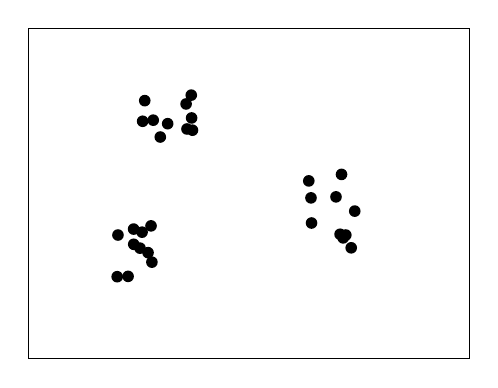
\begin{tikzpicture}[scale=1.4]
			\draw (-0.5,-0.4) rectangle (3.5,2.6);
			
			\fill (0.456,0.778)circle (1.5pt);
			\fill (0.622,0.478)circle (1.5pt);
			\fill (0.457,0.64)circle (1.5pt);
			\fill (0.614,0.807)circle (1.5pt);
			\fill (0.314,0.724)circle (1.5pt);
			\fill (0.533,0.75)circle (1.5pt);
			\fill (0.514,0.605)circle (1.5pt);
			\fill (0.307,0.346)circle (1.5pt);
			\fill (0.406,0.349)circle (1.5pt);
			\fill (0.587,0.564)circle (1.5pt);
			
			\fill (2.065,1.061)circle (1.5pt);
			\fill (2.045,1.215)circle (1.5pt);
			\fill (2.292,1.07)circle (1.5pt);
			\fill (2.381,0.724)circle (1.5pt);
			\fill (2.43,0.608)circle (1.5pt);
			\fill (2.342,1.274)circle (1.5pt);
			\fill (2.329,0.731)circle (1.5pt);
			\fill (2.462,0.941)circle (1.5pt);
			\fill (2.357,0.698)circle (1.5pt);
			\fill (2.07,0.833)circle (1.5pt);
			
			\fill (0.765,1.734)circle (1.5pt);
			\fill (0.557,1.943)circle (1.5pt);
			\fill (0.698,1.613)circle (1.5pt);
			\fill (0.634,1.766)circle (1.5pt);
			\fill (0.979,1.993)circle (1.5pt);
			\fill (0.99 ,1.675)circle (1.5pt);
			\fill (0.538,1.756)circle (1.5pt);
			\fill (0.932,1.913)circle (1.5pt);
			\fill (0.982,1.786)circle (1.5pt);
			\fill (0.94 ,1.686)circle (1.5pt);
		\end{tikzpicture}
		\caption*{\footnotesize Original Set}
		\label{fig:badrep}
	\end{minipage}
	\hspace{1cm}
	\begin{minipage}{0.4\linewidth}
		\centering
		\begin{tikzpicture}[scale=1.4]
		\draw (-0.5,-0.4) rectangle (3.5,2.6);
		
		\fill (0.765,1.734)circle (1.5pt);
		\fill (0.514,0.605)circle (1.5pt);
		\fill (2.292,1.07)circle (1.5pt);
		\end{tikzpicture}		
		\caption*{\footnotesize Representative Subset}
		\label{fig:goodrep}
	\end{minipage}
	\caption{Example of a Representative Set}
	\label{fig:rep}
\end{figure}
\paragraph{}
This thesis aims to research, develop, and analyse different algorithms to choose a representative subset of geographic points, whilst being able to dynamically change that set of points via zooming or panning over a geographic region containing a large amount of geographical data. Should optimal solution algorithms prove too slow, heuristic approaches will be employed. Heuristic algorithms will have their solution quality and speed benchmarked against implicit enumeration algorithms.
Whichever algorithm is deemed the best will be implemented in the web framework via the \emph{WFS} and \emph{WMS} web mapping standards.
\paragraph{}
This report is organized as follows:
Chapter \ref{chap:theory} - \nameref{chap:theory} defines the base theoretical concepts, such as a notion of representativeness, as well as some useful structures used in the algorithms. Chapter \ref{chap:sota} - \nameref{chap:sota} analyses previous related work. Chapter \ref{chap:algos} - \nameref{chap:algos} describes the implicit enumeration algorithms implemented so far, as well as an analysis on their time and space complexities. Chapter \ref{chap:future} - \nameref{chap:future} describes the direction of the heurisitc algorithms to be developed in the second half of the thesis. 
\chapter{Concepts, Definitions and Notation}
\label{chap:theory}
\lhead{Chapter \ref{chap:theory}. \emph{\nameref{chap:theory}}}
This chapter gives an introduction to the base concepts used further in this report.
The chapter starts by establishing the formal definition of the problem at hand. 
Then it proceeds to detail the algorithmic and geometric concepts to be used in the different approaches described in the following chapters.
\section{Definitions of Coverage}
\label{sect:problem}
Representativeness consists of finding a subset of points in a larger set. The subset chosen should be able to keep some specified properties of the original set, such as density, or general distribution. As such there can be many ways to define representativeness. For the purposes of this thesis, we will use the definition of \emph{coverage}.
Given a set of points $N$ in $\mathbb{R}^2$, we must choose a subset, $P$, that best matches our definition of representativeness. The size of $P$, however, is constrained to a size $k$, which specifies how many points can be displayed in a section of a map.

For any point in $N$ not in $P$, there must be a point in $P$ that best represents it. In a geographic or geometric plane, this notion of representativeness may be defined by the distance, i.e.\ the point $p$ that best represents $q$ is the closest point closest to $q$, under some notion of distance. 
Although the points represent geographic locations, the metric that would measure their distance on the surface of the globe, the geodesic distance, will not be used in this thesis. The triangular inequality property does not apply to geodesic distances as a sphere (or an approximation of thereof) is not an Euclidean space, and it would add an unnecessary layer of complexity to computing the coverage.
Because of this, in this thesis, the coordinates of the points are the planar projection of the geographic coordinates to their location counterparts, as implemented by the WMS and WFS web mapping standards. Therefore, the Euclidean norm will be used as the spatial distance notion. 

Finding the most representative set $P$ in $N$ will mean that every point in $N$ will be assigned to the point in $P$ closest to it. This definition of representativeness is referred to as \emph{coverage} and the points in $P$ are called \emph{centroids}.

The coverage value of a given centroid is defined by the circle around that centroid with the radius defined by the distance between itself and the farthest non-centroid point assigned to it. The coverage value of a subset is determined by the highest coverage value of its points. It can thus be more formally described as:

\begin{equation}
\max_{n \in N}
	{\min_{p \in P}
		{\lVert p-n \rVert}
	}
\end{equation}

%\paragraph{}
\noindent
where $N$ is the initial set of points in $\mathbb{R}^2$, $P$ is the centroid subset and $\lVert \cdot \rVert $ is the Euclidean distance.
The most representative subset, however, is the one with the minimum value of coverage. This means all points will be assigned to the closest centroid, minimising the coverage of all centroids and avoiding overlapping coverage areas whenever possible.
We can then finally define our problem as the minimising the coverage:

\begin{equation}
\min_{\substack{P \subseteq N\\ \lvert P \rvert = k}}{\max_{n \in N}{\min_{p \in P}{\lVert p-n \rVert}}}
\end{equation}

This is known in the field of optimisation as the \emph{k-centre} problem, and is an example of a facility location problem \cite{thisfref}. Figure \ref{fig:cov} shows two possible centroid assignments, each with its own value of coverage, $d$.

\begin{figure}[H]
	\centering
	\begin{minipage}{0.45\linewidth}
		\centering
		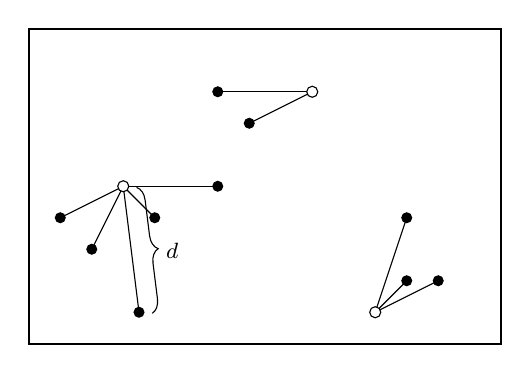
\begin{tikzpicture}[scale=0.4]
		
		\draw [<->,thick] (0,0) rectangle (15,10) {};
		%centroids
		
		%Left Group
%		\fill ( 7,7) circle (5pt);
		\fill ( 1,4) circle (5pt);
		\fill ( 4,4) circle (5pt);
		\fill ( 2,3) circle (5pt);
		\fill (3.5,1) circle (5pt);
		\fill ( 6,5) circle (5pt);
		
		%Middle Group
		
		\fill ( 7,7) circle (5pt);
		\fill ( 6,8) circle (5pt);
		
		%Right Group
		\fill (12,2) circle (5pt);
		\fill (12,4) circle (5pt);
		\fill (13,2) circle (5pt);
		
		%Lines
		\draw [-] (1,4) -- (3,5);
		\draw [-] (4,4) -- (3,5);
		\draw [-] (2,3) -- (3,5);
		\draw [-] (3.5,1) -- (3,5);
		\draw [-] (6,5) -- (3,5);
		
		\draw [-] (7,7) -- (9,8);
		\draw [-] (6,8) -- (9,8);
		
		\draw [-] (12,2) -- (11,1);
		\draw [-] (12,4) -- (11,1);
		\draw [-] (13,2) -- (11,1);
		\fill [white] (11,1) circle (5pt);
		\fill [white] ( 3,5) circle (5pt);
		\fill [white] ( 9,8) circle (5pt);
		
		\draw (11,1) circle (5pt);
		\draw ( 3,5) circle (5pt);
		\draw ( 9,8) circle (5pt);
		
		\draw [decorate,decoration={brace,amplitude=5pt},xshift=12pt,yshift=-1pt]
		(3,5) -- (3.5,1)node [black,midway,xshift=10pt] {\footnotesize$d$};
		\end{tikzpicture}
		\caption*{Non-Optimal Assignment}
		\label{fig:badcov}
	\end{minipage}
	\begin{minipage}{0.45\linewidth}
		\centering
		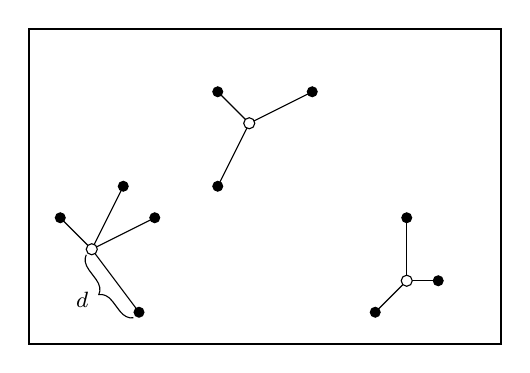
\begin{tikzpicture}[scale=0.4]
		
		\draw [<->,thick] (0,0) rectangle (15,10) {};
		%centroids
		
		%Left Group
		\fill ( 1,4) circle (5pt);
		\fill ( 4,4) circle (5pt);
		\fill ( 3,5) circle (5pt);
		\fill (3.5,1) circle (5pt);
		
		%Middle Group
		\fill ( 6,5) circle (5pt);
		\fill ( 9,8) circle (5pt);
		\fill ( 6,8) circle (5pt);
		
		%Right Group
		\fill (11,1) circle (5pt);
		\fill (12,4) circle (5pt);
		\fill (13,2) circle (5pt);
		
		%\pause
		%Lines
		\draw [-] (1,4) -- (2,3);
		\draw [-] (4,4) -- (2,3);
		\draw [-] (3,5) -- (2,3);
		\draw [-] (3.5,1) -- (2,3);
		
		\draw [-] (6,5) -- (7,7);
		\draw [-] (9,8) -- (7,7);
		\draw [-] (6,8) -- (7,7);
		
		\draw [-] (11,1) -- (12,2);
		\draw [-] (12,4) -- (12,2);
		\draw [-] (13,2) -- (12,2);
		
		\fill [white] ( 2,3) circle (5pt);
		\fill [white] (12,2) circle (5pt);
		\fill [white] ( 7,7) circle (5pt);
		
		\draw ( 2,3) circle (5pt);
		\draw (12,2) circle (5pt);
		\draw ( 7,7) circle (5pt);
		
		%Circles
		%\draw [dashed] (2,3) circle (2.5);
		%\draw [dashed] (7,7) circle (2.236);
		%\draw [dashed] (12,2) circle (2);
		%\pause
		\draw [decorate,decoration={brace,amplitude=5pt},xshift=-5pt,yshift=-5pt]
		(3.5,1) -- (2,3)node [black,midway,xshift=-10pt,yshift=-5pt] {\footnotesize$d$};
		\end{tikzpicture}		
		\caption*{Optimal Assignment}
		\label{fig:goodcov}
	\end{minipage}
	\caption{Different assignments for the same set of points}
	\label{fig:cov}
\end{figure}

For the 1-dimensional case, the minimum coverage value can be calculated in polynomial time \cite{dvaz}. However, for any other number of dimensions it is a \emph{NP-hard} problem, and cannot be solved in polynomial time \cite{complex}.

\section{Algorithmic Concepts}
\subsection{Branch-and-Bound}
Minimising coverage, as shown, is a \emph{NP-hard} combinatorial problem \cite{complex}. One possible way of solving the problem is to use implicit enumeration algorithms such as \emph{Branch-and-Bound} algorithms.
These algorithms solve the problems by recursively dividing the solution set in half, thus \emph{branching} it into a rooted binary tree.
At each step of the subdivision, it then calculates the upper and lower bounds for the best possible value for the space of solutions considered at that node. This step is called \emph{bounding}.
In the case of a minimisation problem, it would be the upper and lower bounds for minimum possible value for the objective function in the current node. These values are then compared with the best ones already calculated in other branches of the recursive tree, and updated if better.

The bounds can be used to \emph{prune} the search tree. This can be done when the branch-and-bound algorithm arrives at a node where the lower bound is larger than the best calculated upper bound. At this point, no further search within the branch is required, as there is no solution in the current branch better than one that has already been calculated. 
In the case that the global upper and lower bound meet, the algorithm has arrived at the best possible solution, and no further computation must be done.

These algorithms are very common in the field of optimisation and can be very efficient, but their performance depends on the complexity and tightness of its bounds. Tighter bounds accelerate the process, but are usually slower to compute, so a compromise has to be made in order to obtain the fastest possible algorithm.

\subsection{Approximation Algorithms}
\change{Optimal solution algorithms, even very optimized ones, are oftentimes still too inefficient to be used in any practical, time constrained application. One possible strategy to solve an \emph{NP-hard} problem is to use an \emph{approximation algorithm}.}

\change{Approximation algorithms do not compute the optimal solution to a given problem. Instead, for the sake of time efficiency, these algorithms are designed to compute a solution that differs from the optimal by a given factor. For example, a 2-approximation algorithm for a minimising problem will not compute any solution that is more than double the optimal value for any given input. By compromising the quality of the solution, the algorithms can end within polynomial time.}\change{}

\section{Geometric Concepts and Geometric Structures}
In the following, we explain some geometric concepts that are used in the following chapters, in order to simplify the explanation of more complex algorithms in further chapters.
\subsection{Nearest Neighbour Search and Point Location}
A common concept in computational geometry is point location. A point location algorithm finds the region on a plane that contains a given point $p$. Depending on the nature and shape of the regions, point location algorithms may differ in approach. In this thesis, most point location problems consist of finding the closest centroid to a given point, i.e.\ a nearest neighbour search algorithm.

Given a point $p$, a \emph{nearest neighbour search} algorithm returns the closest point to $p$ in a given set. Since we need to find the closest centroid to a given point in order to find the correct coverage value, this operation will be one of the most used, and  so we need a fast and flexible way of determining which of the centroids is closest, in order to reduce computational overhead. 

Point location algorithms direct the nearest neighbour search to smaller regions, bypassing any regions that are too distant from $p$, thus reducing the number of calculations necessary to get the proper point location.
Common structures used for point location are \emph{k-d trees} as described in \citet{incrementalcov}. A \emph{k-d tree} partitions the space using a divide and conquer approach to define orthogonally aligned half-planes. This approach takes $\bigo(\log{n})$ time to achieve point location queries. However, a \emph{k-d tree} needs to be periodically updated in order to keep its efficiency and cannot be constructed or deconstructed incrementally without considering this overhead.
\subsection{\textit{k}-Dimensional Trees}
\change{
A \textit{k}-dimensional tree, or \kdtree, is a space partitioning structure used for point location and nearest neighbour queries. A \kdtree is a binary tree, which each of whose nodes represents an axis-aligned hyper-rectangle. Each node specifies an axis and splits the set of points based on whether their coordinate along that axis is greater than or less than a particular value. The axis chosen to split each subgroup is chosen via a rotation system, which in the 2-dimensional space means that each level alternates between the vertical and horizontal axis.}

\change{
During construction, the splitting point is chosen to be the point whose relevant coordinate best divides the group intro two subgroups. The best possible choice for the splitting point at each level is the point which has the median of the relevant coordinate in the group. This ensures that each node divides the number of points in half for so that the resulting tree becomes balanced, and that each point is reachable by performing $\bigo(\log{n})$ operations.
}

\subsubsection*{Construction}
\change{Constructing a \kdtree requires selecting a pivot, which divides the set into two groups: the points whose relevant coordinate is smaller than the pivot, the points whose relevant coordinate is larger than the pivot. The same process is then repeated recursively for each of the groups, alternating the relevant coordinate between both axes. Each recursive call fixes one pivot, which ideally will contain the median value of the relevant coordinate. The time complexity of the construction of a \kdtree relies on the pivot selection function. Calculating the median usually requires sorting a list of $n$ and then picking the $n/2$th element. Since sorting algorithms typically take $\bigo(n \log{n})$, building a \kdtree would take $\bigo(n^2)$ time. To achieve better time complexity and performance the median of medians algorithm described in \ref{median} can be used.
}

\change{
Even though the median of medians algorithm does not necessarily return the actual median, the query complexity in a \kdtree constructed using this still achieves the $\bigo(\log{n})$. This occurs because the median of medians always outputs a value between the $30$th and $70$th percentile. This guarantees that at each level of the \kdtree the group of points covered by each of the children nodes is substantially smaller than the parent node by a constant factor, and there will never be a redundant node that covers the same set of points the parent does. At each level of a given query, each decision discards at least 30\% of the points, maintaining the $\bigo(\log{n})$ time complexity. \cite{kdmedian}
}


\subsection{Median of Medians}
\label{median}
\change{
Efficiently constructing a balance \kdtree depends on an efficient method to pick the point that divides the hyper-rectangle in two. One way to reasonably quickly find a value close to the median is to find the median of a sample. To ensure the quality of this sample, is to gather the medians of smaller subsets which can be quickly calculated. This algorithm is an example of a \emph{selection algorithm} \cite{selection} and is known as the \emph{median of medians} algorithm \cite{medians}.}

\change{
The median of medians algorithms works as follows. Any starting array $S$ consisting of $n$ arbitrary values is split into $n/5$ sub-arrays, each containing at most 5 elements (the last array might have less, depending on whether $n$ is divisible by 5 or not). For each of the sub-arrays, the median can be calculated in constant time, since for 5 values it can be done in at most 6 comparisons, which for the whole array $S$ takes $6n/5$ comparisons. After finding all the sub-arrays' medians and gathering them in a new array $F$, the algorithm then is called recursively for $F$ until only one value $M$ remains. $M$ is then used to partition the input into two sub-groups: elements smaller than $M$ and elements larger than $M$. The two subgroups are then concatenated in increasing order and with $M$ in between them, and the algorithm is recursively called again for the group that contains the $n/2$th point of the newly concatenated list. Whenever the list has less than a given number of elements, the median is calculated via brute-force, to avoid infinite recursion. This value will be the value returned by the initial recursive call of the function.
}

\change{As stated above, this algorithm only returns a value close to the real median. Despite this, it can proven that for any array $S$, the value $M$ will always be between the 30th and the 70th percentiles. At each recursive stage, the values in $F$ larger than $M$ are discarded. This means that out of the $n/5$ values for any given vector, $n/10$ will be larger by definition, since $M$ is picked as the median. For each value in $F$ larger than $M$, there will also be two other values that are larger than $M$, since each value in $F$ was chosen as a median out of 5 different values. This means that the number of values greater than $M$ will be at most $3n/10$. Similarly, by a symmetric proof, there will also be $3n/10$ values in $S$ smaller than $M$. This also means that the second recursive call will at worst have $7n/10$ elements, which is a constant fraction of the input. This property is essential in proving the linear complexity of the algorithm.
}

\change{Analyzing the time complexity $T()$ of this algorithm requires analyzing separatly both recursive calls of the algorithm. The first recursive call occurs in a list of size $n/5$, and takes $T(n/5)$ time. The second recursive call occurs in a list with $7n/10$ elements, which takes $T(7/n)$. Finding the median for a group of 5 elements requires a constant number of comparisons. These comparisons can be arranged in such way that only 6 are necessary for a group of 5 elements. This means that the algorithm has a constant factor of $6/5$ for calculating a median on its smallest division. $T(n)$ is then given by:}
\begin{align}
T(n) \le 6n/5 + T(n/5) + T(7n/10)
\end{align}

\change{If $T(n)$ has, in fact, linear time complexity, then there is a constant $c$ such that: }
\begin{align}
\begin{aligned}
T(n) & \le 6n/5 + cn/5 + 7cn/10\\
     & \le n(12/5 + 9c/10)
\end{aligned}
\end{align}
\change{If $T(n)$ is to be at most $cn$, so that the induction proof is valid, then is must be true that:}
\begin{align}
\begin{aligned}
    n (6/5 + 9c/10) & \le cn \\
    6/5 + 9c/10 & \le c \\
    6/5 & \le c/10 \\
    c & \le 12 \\
\end{aligned}
\end{align}

\change{This proves that $T(n) \le 12n$, or any larger constants than 12 multiplied by $n$ comparisons.}

%http://www.ics.uci.edu/~eppstein/161/960130.html  \cite{eppstein}


\subsection{Voronoi Diagrams}
Voronoi diagrams \cite{tricard2} partition the space into regions, which are defined by the set of points in the space that are closest to a subset of those points. Definitions of distance and space may vary, but on our case we will consider the $\mathbb{R}^2$ plane and the Euclidean distance.
Figure \ref{fig:vd1} shows a partitioning of a plane using a Voronoi Diagram for a set of points:
\begin{figure}[H]
	\begin{center}
		\begin{tikzpicture}[scale=0.4]
		%\draw [<->,thick] (0,10) node (yaxis) [left] {}
		%|- (15,0) node (xaxis) [below] {};
		%centroids
		\fill ( 2, 7) circle (3pt);
		\fill ( 5, 3) circle (3pt);
		\fill ( 6, 9) circle (3pt);
		\fill ( 8, 4) circle (3pt);
		\fill (10, 1) circle (3pt);
		\fill (11, 8) circle (3pt);
		\fill (13, 5) circle (3pt);
		\fill (13,10) circle (3pt);
		\fill (15, 7) circle (3pt);
		\fill (16, 3) circle (3pt);
		
		\draw [-] ( 5.6764, 5.9706) -- ( 4.9545, 6.0909);
		\draw [-] ( 5.6764, 5.9706) -- ( 8.1956, 6.9783);
		\draw [-] (10.3235, 5.3824) -- ( 8.1956, 6.9783);
		\draw [-] (10.3235, 5.3824) -- (10.6765, 3.6176);
		\draw [-] ( 7.2272, 1.3182) -- (10.6765, 3.6176);
		\draw [-] ( 7.2272, 1.3182) -- ( 5.6764, 5.9706);
		\draw [-] (13.0556, 1.3182) -- (10.6765, 3.6176);
		\draw [-] (13.0556, 1.3182) -- (15.1000, 4.9000);
		\draw [-] (12.9000, 7.1000) -- (15.1000, 4.9000);
		\draw [-] (12.9000, 7.1000) -- (10.3235, 5.3824);
		\draw [-] (12.9000, 7.1000) -- (13.1000, 7.9000);
		\draw [-] ( 9.1667,11.8333) -- (13.1000, 7.9000);
		\draw [-] ( 9.1667,11.8333) -- ( 8.1956, 6.9783);

		\draw [-,dashed] ( 4.9545, 6.0909) -- (2 , 12);
		\draw [-,dashed] ( 4.9545, 6.0909) -- (0, 2.375);
		\draw [-,dashed] ( 7.2272, 1.3182) -- ( 6.7, 0);
		\draw [-,dashed] (13.0556, 1.3182) -- (13.6667, 0);
		\draw [-,dashed] (15.1000, 4.9000) -- (18, 5.625);
		\draw [-,dashed] (13.1000, 7.9000) -- (18, 11.1667);
		\draw [-,dashed] ( 9.1667,11.8333) -- ( 9.1429, 12);
		
		\end{tikzpicture}
	\end{center}
	\caption{Example of a Voronoi Diagram}
	\label{fig:vd1}
\end{figure}
\noindent
Dashed lines extend to infinity. Any new point inserted in this plane is contained in one of the cells, and its closest point is the one at the centre of the cell.
Each edge is the perpendicular bisector between two neighbouring points, dividing the plane in two half planes, containing the set of points closest to each of them.
The construction of Voronoi diagrams can be done incrementally, but in order to obtain fast query times, one needs to decompose the cells into simpler structures. 
\subsection{Delaunay Triangulations}
Another useful structure for geometric algorithms is the Delaunay triangulation \cite{tricard2}.
A Delaunay triangulation \cite{delbible} is a special kind of triangulation with many useful properties. 
In an unconstrained Delaunay triangulation, each triangle's circumcircle contains no points other inside its circumference.

A Delaunay triangulation maximizes the minimum angle of its triangles, avoiding long or slender ones.
The set of all its edges contains both the minimum-spanning tree and the convex hull.
The Delaunay triangulation is unique for a set of points, except when it contains a subset that can be placed along the same circumference. Figure \ref{fig:dt1} shows the Delaunay triangulation of the same set of points used in Figure \ref{fig:vd1}:
\begin{figure}[!h]
	\begin{center}
		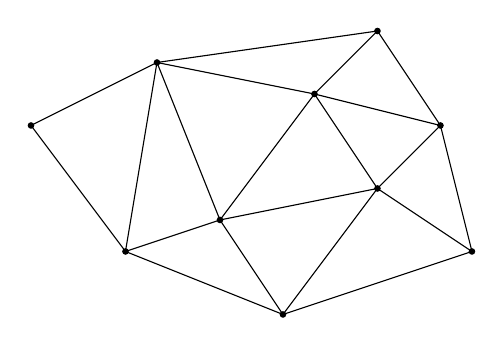
\begin{tikzpicture}[scale=0.4]
		%\draw [<->,thick] (0,10) node (yaxis) [left] {}
		%|- (15,0) node (xaxis) [below] {};
		%centroids
		\fill ( 2, 7) circle (3pt);
		\fill ( 5, 3) circle (3pt);
		\fill ( 6, 9) circle (3pt);
		\fill ( 8, 4) circle (3pt);
		\fill (10, 1) circle (3pt);
		\fill (11, 8) circle (3pt);
		\fill (13, 5) circle (3pt);
		\fill (13,10) circle (3pt);
		\fill (15, 7) circle (3pt);
		\fill (16, 3) circle (3pt);
		
		
		\draw [-] ( 2,7) -- ( 6,9);
		\draw [-] ( 6,9) -- ( 5,3);
		\draw [-] ( 5,3) -- ( 2,7);
		\draw [-] ( 6,9) -- ( 8,4);
		\draw [-] (10,1) -- ( 8,4);
		\draw [-] ( 5,3) -- (10,1);
		\draw [-] ( 8,4) -- ( 5,3);
		\draw [-] ( 8,4) -- (11,8);
		\draw [-] (11,8) -- (6,9);
		\draw [-] ( 6,9) -- (13,10);
		\draw [-] (11,8) -- (13,10);
		\draw [-] (15,7) -- (13,10);
		\draw [-] (16,3) -- (15,7);
		\draw [-] (16,3) -- (10,1);
		\draw [-] (16,3) -- (13,5);
		\draw [-] (13,5) -- (15,7);
		\draw [-] (13,5) -- (10,1);
		\draw [-] (13,5) -- (8,4);
		\draw [-] (13,5) -- (11,8);
		\draw [-] (15,7) -- (11,8);
		\end{tikzpicture}
	\end{center}
	\caption{Example of a Delaunay Triangulation}
	\label{fig:dt1}
\end{figure}
\noindent
More importantly, the Delaunay triangulation of a set of points is the dual graph of its Voronoi Diagram. The edges of the Voronoi diagram, are the line segments connecting the circumcentres of the Delaunay triangles. When overlapped, the duality becomes more obvious. Figure \ref{fig:dt_vd} shows the overlapping of the Voronoi diagram in Figure \ref{fig:vd1} and the Delaunay  triangulation in Figure \ref{fig:dt1}. The Delaunay edges, in black, connect the points at the centre of the Voronoi cells, with edges in blue, to their neighbours.
\begin{figure}[H]
	\begin{center}
		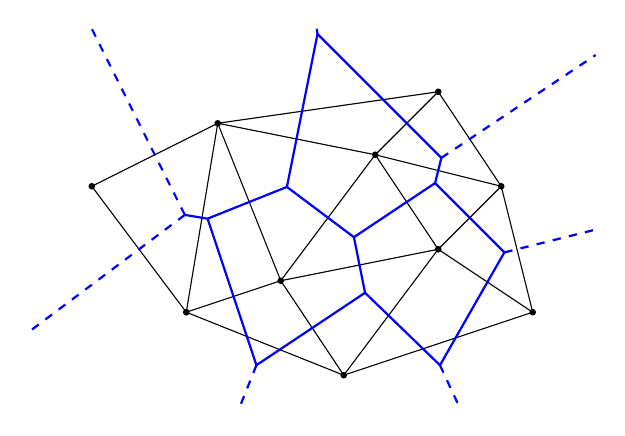
\begin{tikzpicture}[scale=0.4]
		%\draw [<->,thick] (0,10) node (yaxis) [left] {}
		%|- (15,0) node (xaxis) [below] {};
		%centroids
		\fill ( 2, 7) circle (3pt);
		\fill ( 5, 3) circle (3pt);
		\fill ( 6, 9) circle (3pt);
		\fill ( 8, 4) circle (3pt);
		\fill (10, 1) circle (3pt);
		\fill (11, 8) circle (3pt);
		\fill (13, 5) circle (3pt);
		\fill (13,10) circle (3pt);
		\fill (15, 7) circle (3pt);
		\fill (16, 3) circle (3pt);
		
		%DELAUNAY
		\draw [-] ( 2,7) -- ( 6,9);
		\draw [-] ( 6,9) -- ( 5,3);
		\draw [-] ( 5,3) -- ( 2,7);
		\draw [-] ( 6,9) -- ( 8,4);
		\draw [-] (10,1) -- ( 8,4);
		\draw [-] ( 5,3) -- (10,1);
		\draw [-] ( 8,4) -- ( 5,3);
		\draw [-] ( 8,4) -- (11,8);
		\draw [-] (11,8) -- (6,9);
		\draw [-] ( 6,9) -- (13,10);
		\draw [-] (11,8) -- (13,10);
		\draw [-] (15,7) -- (13,10);
		\draw [-] (16,3) -- (15,7);
		\draw [-] (16,3) -- (10,1);
		\draw [-] (16,3) -- (13,5);
		\draw [-] (13,5) -- (15,7);
		\draw [-] (13,5) -- (10,1);
		\draw [-] (13,5) -- (8,4);
		\draw [-] (13,5) -- (11,8);
		\draw [-] (15,7) -- (11,8);
		
		%VORONOI		
		\draw [-,blue,thick] ( 5.6764, 5.9706) -- ( 4.9545, 6.0909);
		\draw [-,blue,thick] ( 5.6764, 5.9706) -- ( 8.1956, 6.9783);
		\draw [-,blue,thick] (10.3235, 5.3824) -- ( 8.1956, 6.9783);
		\draw [-,blue,thick] (10.3235, 5.3824) -- (10.6765, 3.6176);
		\draw [-,blue,thick] ( 7.2272, 1.3182) -- (10.6765, 3.6176);
		\draw [-,blue,thick] ( 7.2272, 1.3182) -- ( 5.6764, 5.9706);
		\draw [-,blue,thick] (13.0556, 1.3182) -- (10.6765, 3.6176);
		\draw [-,blue,thick] (13.0556, 1.3182) -- (15.1000, 4.9000);
		\draw [-,blue,thick] (12.9000, 7.1000) -- (15.1000, 4.9000);
		\draw [-,blue,thick] (12.9000, 7.1000) -- (10.3235, 5.3824);
		\draw [-,blue,thick] (12.9000, 7.1000) -- (13.1000, 7.9000);
		\draw [-,blue,thick] ( 9.1667,11.8333) -- (13.1000, 7.9000);
		\draw [-,blue,thick] ( 9.1667,11.8333) -- ( 8.1956, 6.9783);
		
		\draw [-,blue,thick,dashed] ( 4.9545, 6.0909) -- (	2.0000,12.0000);
		\draw [-,blue,thick,dashed] ( 4.9545, 6.0909) -- (	0.0000,	2.3750);
		\draw [-,blue,thick,dashed] ( 7.2272, 1.3182) -- (	6.7000, 0.0000);
		\draw [-,blue,thick,dashed] (13.0556, 1.3182) -- (13.6667, 0.0000);
		\draw [-,blue,thick,dashed] (15.1000, 4.9000) -- (18.0000, 5.6250);
		\draw [-,blue,thick,dashed] (13.1000, 7.9000) -- (18.0000,11.1667);
		\draw [-,blue,thick,dashed] ( 9.1667,11.8333) -- ( 9.1429,12.0000);
		
		\end{tikzpicture}
	\end{center}
	\caption{Overlap of a Voronoi Diagram and its Delaunay Triangulation}
	\label{fig:dt_vd}
\end{figure}
\noindent
Unlike its counterpart, the Delaunay is much simpler to build incrementally. It is also easier to work with, whilst still providing most of the Voronoi diagram's properties, including the ability to calculate both point location and nearest neighbour searches.
\subsubsection*{Construction}
\label{sect:dtconst}

There are many algorithms to construct a Delaunay triangulation. 
The particular conditions of our approach to the coverage problem impose some restrictions to the choice of the algorithm to use.
Building a Delaunay triangulation can be done incrementally. Starting with a valid triangulation, points can be added, creating and updating existing triangles. An efficient way to do so is to use the Bowyer-Watson algorithm \cite{bwalgo}.

Starting with a valid Delaunay triangulation $\mathcal{T}$, we find the triangle $t$ with vertices $a$,$b$ and $c$ that contains the vertex to insert $v$ using a point location algorithm, such as the line walking algorithm described in the previous section. We then follow algorithm \ref{alg:bowyer} for each vertex $v$ to be included in the triangulation:
\begin{algorithm}[H]
    \caption{Bowyer-Watson Algorithm}
    \begin{algorithmic}[1]
        \Procedure {InsertVertex}{$v,a,b,c$}
            \State $\text{DeleteTriangle}(a,b,c)$
            \State $\text{DigCavity}(v,a,b)$
            \State $\text{DigCavity}(v,b,c)$
            \State $\text{DigCavity}(v,c,a)$
        \EndProcedure
    \end{algorithmic}
    
    \begin{algorithmic}[1]
       	\Procedure {DigCavity}{$a,b,c$}
        	\State $d \gets \text{Adjacent}(b,c)$
        	\If {$d \neq \varnothing$}
	        	\If {$\text{inCircle}(a,b,c,d)$}
		        	\State $\text{DeleteTriangle}(w,v,x)$
		        	\State $\text{DigCavity}(a,b,d)$
		        	\State $\text{DigCavity}(a,d,c)$
	        	\Else 
		        	\State$\text{AddTriangle}(a,b,c)$
	        	\EndIf
        	\EndIf
       	\EndProcedure
    \end{algorithmic}
    \label{alg:bowyer}
\end{algorithm}

The algorithm starts by removing the triangle $t$ that contains the new vertex $v$, and recursively checks adjacent triangles whose circumcircle contains $v$ using the \emph{DigCavity} function. Any triangle that contains $v$ in its circumcircle (calculated with the \emph{InCircle} function), violates the Delaunay rule, and must also be deleted and have its sides recursively checked, until no adjacent triangles violate the Delaunay rule. Whenever the \emph{DigCavity} function reaches a set of three points whose circumcircle does not contain $v$, it creates the triangle by creating counter-clockwise half-edges between those three points (\emph{AddTriangle}). For inserting $n$ points, this algorithm has an expected time complexity of $\bigo(n \log n)$ and is described in more detail by \citet{tricomplex}.

\subsubsection*{Deconstruction}
Deconstructing a Delaunay triangulation usually consists of reversing the construction algorithm to remove points from the triangulation. However, as we will explain in a later chapter, in our case the deconstruction has to be incremental. Since the first point to be removed from the triangulation is necessarily the last one to be inserted, we can use a simpler approach. 
At each step of the construction, all created and removed edges and triangle from the triangulation can be stored in a LIFO structure, or a stack. When the last inserted point is to be removed, recreating the previous state of the triangulation is only a matter of rolling back and retrieving the information from the stack. This also means no geometrical calculations have to be performed, and the old edges and triangles are quickly put back in place, with no new memory allocation needed.

\subsubsection*{Half-Edge Structure}
A useful structure to use when building and managing triangulation meshes is the half-edge structure. The half-edge structure represents one orientation of each edge in the triangulation. This means that for each pair of points ($p_i,p_j$)connected in a triangulation $\mathcal{T}$, there are two directed half-edges: one represents the edge from $p_i$ to $p_j$, and the other represents the opposite direction, connecting $p_j$ to $p_i$. They both contain information about the triangle that they face, and thus, are part of. Triangles are defined by three half edges. All the half edges in the triangle share two of the vertices of the triangle, and are all sorted in a counter-clockwise order. 
Figure \ref{fig:hedge} further illustrates the concept of the half-edges.\\
\begin{figure}[!h]
	\begin{center}
		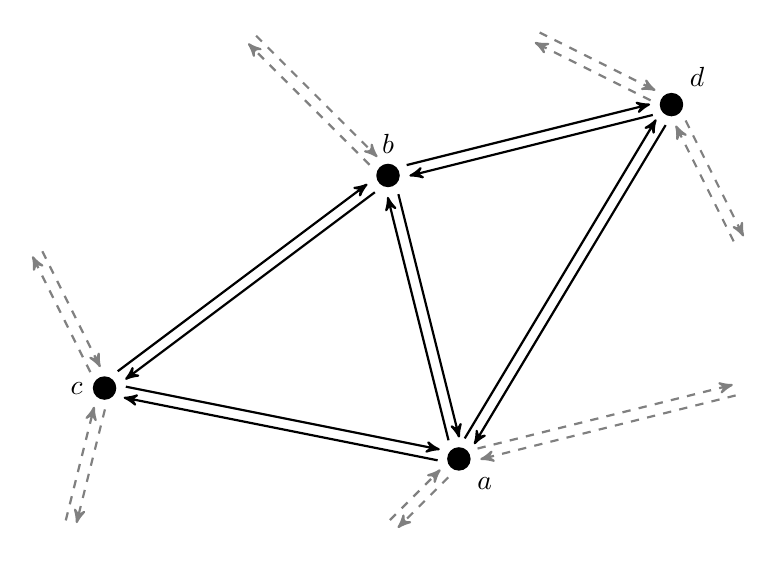
\begin{tikzpicture}[scale=0.9,
		arr/.style={->,>=stealth',thick,black,shorten >=3pt,shorten <=3pt},
		edg/.style={black,shorten >=6pt,shorten <=6pt},
		par/.style={decoration={sl,raise=2pt},decorate}]
		
		\node [fill,circle,inner sep=3pt,label=below right:$a$] (A) at (6,1){};
		\node [fill,circle,inner sep=3pt,label=above: $b$] (B) at (5,5){};
		\node [fill,circle,inner sep=3pt,label=left: $c$] (C) at (1,2){};
		\node [fill,circle,inner sep=3pt,label=above right:$d$] (D) at (9,6){};
		
		\path[->,>=latex]
		(A) edge [arr,par](B)
		(B) edge [arr,par](C)
		(C) edge [arr,par](B)
		(C) edge [arr,par](A)
		(A) edge [arr,par](C)
		
		(B) edge [arr,par](A)
		(A) edge [arr,par](D)
		(D) edge [arr,par](B)
		(D) edge [arr,par](A)
		(B) edge [arr,par](D);
		\draw [arr,par,dashed,gray] (B) -- (3,7);
		\draw [arr,par,dashed,gray] (3,7) -- (B);
		
		\draw [arr,par,dashed,gray] (C) -- (0.5,0);
		\draw [arr,par,dashed,gray] (0.5,0) -- (C);
		
		\draw [arr,par,dashed,gray] (C) -- (0,4);
		\draw [arr,par,dashed,gray] (0,4) -- (C);
		
		\draw [arr,par,dashed,gray] (A) -- (5,0);
		\draw [arr,par,dashed,gray] (5,0) -- (A);
		
		\draw [arr,par,dashed,gray] (A) -- (10,2);
		\draw [arr,par,dashed,gray] (10,2) -- (A);
		
		\draw [arr,par,dashed,gray] (D) -- (10,4);
		\draw [arr,par,dashed,gray] (10,4) -- (D);
		
		\draw [arr,par,dashed,gray] (D) -- (7,7);
		\draw [arr,par,dashed,gray] (7,7) -- (D);

		
%		\path[-,color=gray]
%		(A) edge (B)
%		(B) edge (C)
%		(C) edge (A)
%		(A) edge (D)
%		(D) edge (B)		
%		;
		\end{tikzpicture}
	\end{center}
	\caption{Illustration of the Half-Edge Structure}
	\label{fig:hedge}
\end{figure}
This structure makes it easier to store the changes to the triangulation at each step, since they contain the information about the triangles themselves. This means that only the half edges need to be stored in the stack (for construction and deconstruction) with no need to manage the triangles directly.
The half-edge structure helps to obtain the triangulation neighbours for any vertex $v$, since it keeps all the edges starting at any given point easily accessible. All neighbours to any point $v$ are the end points to the half-edges starting at $v$. This property is useful when efficiently implementing the greedy routing algorithm described in the following Section. 

\subsubsection*{Greedy Routing}
\label{r:gr}
In order to quickly calculate the nearest neighbour to a point in a set, one can make use of the Delaunay triangulation with Greedy Routing \cite{greedyroute}.
Consider a triangulation $\mathcal{T}$. In order to find the closest vertex in $\mathcal{T}$ to a new point $p$, start at an arbitrary vertex of $\mathcal{T}$, $v$, and find a neighbour $u$ of $v$ whose distance to $p$ is smaller than the distance between $p$ and $v$. Repeat the process for $u$ and its neighbours. When a point $w$ is reached such that no neighbours of $w$ are closer to $p$ than $w$ is, the closest point to $p$ in $\mathcal{T}$ has been found. In the following, we show that the greedy routing algorithm is correct:
\begin{figure}[H]
	\begin{center}
		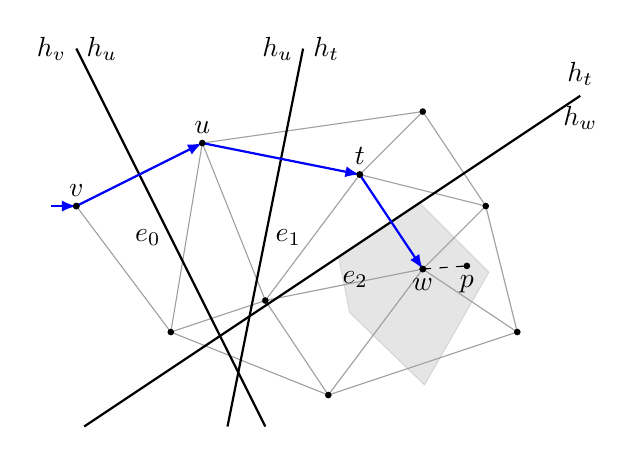
\begin{tikzpicture}[scale=0.4]
		%\draw [<->,thick] (0,10) node (yaxis) [left] {}
		%|- (15,0) node (xaxis) [below] {};
		
		%VORONOI
%		\draw [-,gray!50] ( 5.6764, 5.9706) -- ( 4.9545, 6.0909);
%		\draw [-,gray!50] ( 5.6764, 5.9706) -- ( 8.1956, 6.9783);
%		\draw [-,gray!50] (10.3235, 5.3824) -- ( 8.1956, 6.9783);
%		\draw [-,gray!50] (10.3235, 5.3824) -- (10.6765, 3.6176);
%		\draw [-,gray!50] ( 7.2272, 1.3182) -- (10.6765, 3.6176);
%		\draw [-,gray!50] ( 7.2272, 1.3182) -- ( 5.6764, 5.9706);
%		\draw [-,gray!50] (13.0556, 1.3182) -- (10.6765, 3.6176);
%		\draw [-,gray!50] (13.0556, 1.3182) -- (15.1000, 4.9000);
%		\draw [-,gray!50] (12.9000, 7.1000) -- (15.1000, 4.9000);
%		\draw [-,gray!50] (12.9000, 7.1000) -- (10.3235, 5.3824);
%		\draw [-,gray!50] (12.9000, 7.1000) -- (13.1000, 7.9000);
%		\draw [-,gray!50] ( 9.1667,11.8333) -- (13.1000, 7.9000);
%		%\draw [-,gray!50] ( 9.1667,11.8333) -- ( 8.1956, 6.9783);
%		%VORONOI EXTENDED
%		\draw [-,gray!50] ( 4.9545, 6.0909) -- (2 , 12);
%		\draw [-,gray!50] ( 4.9545, 6.0909) -- (0, 2.375);
%		\draw [-,gray!50] ( 7.2272, 1.3182) -- ( 6.7, 0);
%		\draw [-,gray!50] (13.0556, 1.3182) -- (13.6667, 0);
%		\draw [-,gray!50] (15.1000, 4.9000) -- (18, 5.625);
%		\draw [-,gray!50] (13.1000, 7.9000) -- (18, 11.1667);
%		\draw [-,gray!50] ( 9.1667,11.8333) -- ( 9.1429, 12);
		
		\filldraw[fill=black, opacity=0.1] 	(10.3235, 5.3824) -- (10.6765, 3.6176) --
											(13.0556, 1.3182) -- (15.1000, 4.9000) --
											(12.9000, 7.1000) -- cycle;
		
		%DELAUNAY
		\draw [-,gray!75] ( 2,7) -- ( 6,9);
		\draw [-,gray!75] ( 6,9) -- ( 5,3);
		\draw [-,gray!75] ( 5,3) -- ( 2,7);
		\draw [-,gray!75] ( 6,9) -- ( 8,4);
		\draw [-,gray!75] (10,1) -- ( 8,4);
		\draw [-,gray!75] ( 5,3) -- (10,1);
		\draw [-,gray!75] ( 8,4) -- ( 5,3);
		\draw [-,gray!75] ( 8,4) -- (11,8);
		\draw [-,gray!75] (11,8) -- (6,9);
		\draw [-,gray!75] ( 6,9) -- (13,10);
		\draw [-,gray!75] (11,8) -- (13,10);
		\draw [-,gray!75] (15,7) -- (13,10);
		\draw [-,gray!75] (16,3) -- (15,7);
		\draw [-,gray!75] (16,3) -- (10,1);
		\draw [-,gray!75] (16,3) -- (13,5);
		\draw [-,gray!75] (13,5) -- (15,7);
		\draw [-,gray!75] (13,5) -- (10,1);
		\draw [-,gray!75] (13,5) -- (8,4);
		\draw [-,gray!75] (13,5) -- (11,8);
		\draw [-,gray!75] (15,7) -- (11,8);
		
		
		%POINTS
		
		\fill ( 2, 7) circle (3pt);
		\fill ( 5, 3) circle (3pt);
		\fill ( 8, 4) circle (3pt);
		\fill (10, 1) circle (3pt);
		\fill (11, 8) circle (3pt);
		\fill (13, 5) circle (3pt);
		\fill (13,10) circle (3pt);
		\fill (15, 7) circle (3pt);
		\fill (16, 3) circle (3pt);
		
		%EDGE E
		\draw [-,thick] ( 8,0)		-- node[left]{$e_0$} ( 2, 12)	node[left]		{$h_v$} node[right]{$h_u$};
		\draw [-,thick] ( 6.8,0)	-- node[right]{$e_1$} (9.2,12)	node[left] 		{$h_u$} node[right]{$h_t$};
		\draw [-,thick] ( 2.25,0)	-- node[below right]{$e_2$} (18,10.5)	node[above]{$h_t$} node[below]{$h_w$};
		
		
		\draw [-,dashed]( 13,5) -- ( 14.4, 5.1);
		\draw [->,>=latex,thick,blue]( 1.2,7) -- (  2,7);
		\draw [->,>=latex,thick,blue]( 2,7) -- (  6,9);
		\draw [->,>=latex,thick,blue]( 6,9) -- ( 11, 8);
		\draw [->,>=latex,thick,blue](11,8) -- ( 13, 5);
		\fill (14.4, 5.1) circle (3pt) node[anchor=north]{$p$};
		\fill ( 2, 7)     circle (3pt) node[anchor=south]{$v$};
		\fill ( 6, 9)     circle (3pt) node[anchor=south]{$u$};
		\fill (11, 8)     circle (3pt) node[anchor=south]{$t$};
		\fill (13, 5)     circle (3pt) node[anchor=north]{$w$};
		
		\end{tikzpicture}
	\end{center}
\end{figure}
\noindent
In Figure \ref{fig:gr1}, the search for the closest vertex to $p$ starts at point $v$. From there, point $u$, which is closer to $p$ than $v$ is, is found. The step is repeated, following the blue path until point $w$ is reached. Since no neighbour of $w$ is closer to $p$ than $w$ is, then $p$ must be within the Voronoi cell of point $w$ (shaded light grey).
\begin{theorem}
\cite{greedyroute}
There is no point set whose Delaunay triangulation defeats the greedy routing algorithm.
\begin{proof}
For every vertex $v$ in a triangulation $\mathcal{T}$, let the perpendicular bisector of the line segment defined by $v$ and any neighbour $u$ be called $e$ if there is at least one neighbour of $v$, $u$ closer to $p$ than $v$ is. The line $e$ intersects the line segment $(v,p)$ and divides the plane in two open half planes: $h_v$ and $h_u$. Note that the half plane $h_u$ contains $p$. Delaunay edges connect the Voronoi neighbours and their bisectors define the edges of the Voronoi cells, which are convex polygons. Repeating the process recursively for $u$, if a point $w$ is found, whose neighbourhood contains no points closer to $p$ than itself, then $p$ is contained within all possible open half planes containing $w$, defined by $w$ and all its neighbours. Point $p$ is then by definition located in point $w$'s Voronoi cell. This means that $w$ is the point in $\mathcal{T}$ closest to $p$.
\end{proof}
\end{theorem}
\subsubsection*{Line Walking}
Another point location algorithm to consider is the line walking algorithm \cite{walking}. This algorithm finds a triangle $t$ in a triangulation $\mathcal{T}$ that contains a given point $v$. 
Starting at any triangle $s$, with the geometrical centre $m$, if point $v$ is not contained in $s$, then the line segment $(v,m)$ intersects a finite set of triangles.  
The line segment $(v,m)$ intersects two edges of each triangle in this set, with the exception of $s$ and $t$ where $(v,m)$ only intersects one edge each. 
By iterating through each triangle choosing the neighbour triangle that contains the next edge that intersects $(v,m)$, triangle $t$ can be found in $\bigo(n)$ time.

This algorithm was described by \citet{walking}, and is illustrated in the following figure, where the dark shaded triangles represent the starting and finishing triangles, and the light shaded triangles the path the algorithm takes to find the final triangle that contains the vertex $v$.
\begin{figure}[H]
	\begin{center}
		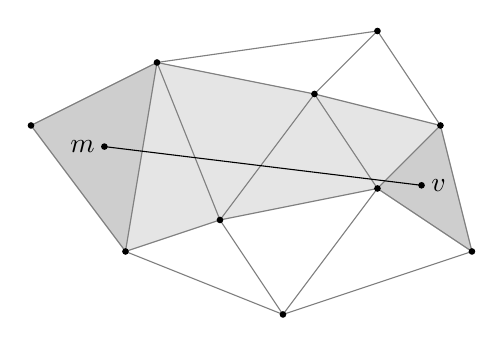
\begin{tikzpicture}[scale=0.4]
		%\draw [<->,thick] (0,10) node (yaxis) [left] {}
		%|- (15,0) node (xaxis) [below] {};
		
		\filldraw[fill=black, opacity=0.1] 	(2,7) -- (6,9) -- 
											(11,8) -- (15,7) -- 
											(16,3) -- (13,5) --
											(8,4) -- (5,3) --
											cycle;
		
		\filldraw[fill=black, opacity=0.1] 	(2,7) -- (6,9) -- (5,3) --
											cycle;
											
		\filldraw[fill=black, opacity=0.1] 	(15,7) -- (13,5) -- (16,3) --
													cycle;
		
		
		
		\draw [-,gray] ( 2,7) -- ( 6,9);
		\draw [-,gray] ( 6,9) -- ( 5,3);
		\draw [-,gray] ( 5,3) -- ( 2,7);
		\draw [-,gray] ( 6,9) -- ( 8,4);
		\draw [-,gray] (10,1) -- ( 8,4);
		\draw [-,gray] ( 5,3) -- (10,1);
		\draw [-,gray] ( 8,4) -- ( 5,3);
		\draw [-,gray] ( 8,4) -- (11,8);
		\draw [-,gray] (11,8) -- (6,9);
		\draw [-,gray] ( 6,9) -- (13,10);
		\draw [-,gray] (11,8) -- (13,10);
		\draw [-,gray] (15,7) -- (13,10);
		\draw [-,gray] (16,3) -- (15,7);
		\draw [-,gray] (16,3) -- (10,1);
		\draw [-,gray] (16,3) -- (13,5);
		\draw [-,gray] (13,5) -- (15,7);
		\draw [-,gray] (13,5) -- (10,1);
		\draw [-,gray] (13,5) -- (8,4);
		\draw [-,gray] (13,5) -- (11,8);
		\draw [-,gray] (15,7) -- (11,8);
		
		
		%centroids
		\fill ( 2, 7) circle (3pt);
		\fill ( 5, 3) circle (3pt);
		\fill ( 6, 9) circle (3pt);
		\fill ( 8, 4) circle (3pt);
		\fill (10, 1) circle (3pt);
		\fill (11, 8) circle (3pt);
		\fill (13, 5) circle (3pt);
		\fill (13,10) circle (3pt);
		\fill (15, 7) circle (3pt);
		\fill (16, 3) circle (3pt);
		
		
		\draw [-]( 4.33,6.33) -- ( 14.4, 5.1);
		%\draw []( 2,7) -- node[anchor=south]{$t$} ( 6,9);
		\fill ( 4.33,6.33) circle (3pt) node[anchor=east]{$m$};
		\fill (14.4, 5.1) circle (3pt) node[anchor=west]{$v$};
		\end{tikzpicture}
	\end{center}
	\caption{Illustration of the Walking Algorithm}
	\label{fig:wk1}
\end{figure}
After finding this triangle, the Bowyer-Watson algorithm described in Section \ref{sect:dtconst} can be used to update the new triangulation, which now includes $v$.
\subsection{Hilbert Curves}

Most of the point location algorithms aforementioned have linear time complexity, and most of the worst case scenarios include searching across the plane. These occur when the starting search position is random and does not make use of the spatial organisation of the data. In order to fully take advantage of these approaches, the points should be sorted is such a way that the distance between consecutive points is minimised.

Hilbert curves are a kind of fractal space-filling curves \cite{sfcurves} that generally minimize the Euclidean distance between points close on the curve.

True Hilbert curves map a 2-dimensional space in a 1-dimension line. This line has an infinite length, which makes mapping 2-dimensional points to it infeasible. Instead, discrete approximations are used. Since the true curve is fractal, the approximations are defined by the number of fractal steps it takes in order to reach them. Figure \ref*{fig:hilbert} demonstrates the first few orders of approximation:
\begin{figure}[H]
	\begin{center}
		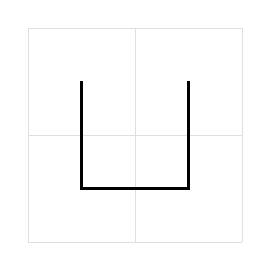
\begin{tikzpicture}[scale=0.17]
		\draw [step=8,gray,very thin,opacity=0.25](0,0) grid(16,16);
		\draw [-,thick] 	(4,12) -- ( 4,4) -- ( 12,4) -- ( 12,12);
		\end{tikzpicture}
		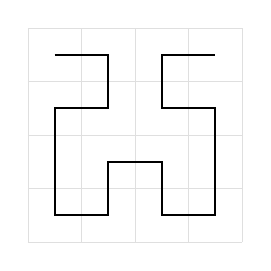
\begin{tikzpicture}[scale=0.17]
		\draw [step=4,gray,very thin,opacity=0.25](0,0) grid(16,16);
		\draw [-,thick]
				 	(2,14) -- ( 6,14) -- (6,10) -- (2,10) -- 
					(2,2)  -- (6,2) -- (6,6) -- (10,6) -- 
					(10,2) -- (14,2) -- (14,10)--(10,10) --
					(10,14) -- (14,14);
		\end{tikzpicture}
		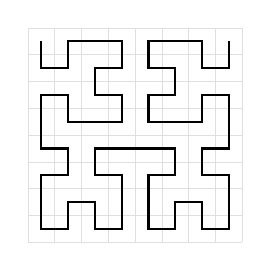
\begin{tikzpicture}[scale=0.17]
		\draw [step=2,gray,very thin,opacity=0.25](0,0) grid(16,16);
		\draw [-,thick] 
					(1,15) 	-- (1,13) 	-- (3,13) 	-- (3,15) 	-- (7,15) 	--
					(7,13) 	-- (5,13) 	-- (5,11)	-- (7,11) 	-- (7,9) 	--
					(3,9) 	-- (3,11)	-- (1,11)	-- (1,7) 	-- (3,7) 	--
					(3,5) 	-- (1,5) 	-- (1,1)	-- (3,1) 	-- (3,3) 	-- 
					(5,3) 	-- (5,1) 	-- (7,1)  	-- (7,5) 	-- (5,5) 	--
					(5,7) 	-- (11,7) 	-- (11,5)  	-- (9,5) 	-- (9,1) 	--
					(11,1)	-- (11,3) 	-- (13,3)  	-- (13,1) 	-- (15,1) 	--
					(15,5) 	-- (13,5) 	-- (13,7)  	-- (15,7) 	-- (15,11)	--
					(13,11)	-- (13,9)  	-- (9,9) 	-- (9,11) 	-- (11,11)	--
					(11,13)	-- (9,13) 	-- (9,15) 	-- (13,15)  -- (13,13) 	--
					(15,13) -- (15,15)
					;
		
		\end{tikzpicture}
		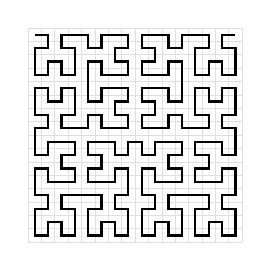
\begin{tikzpicture}[scale=0.17]
		\draw [step=1,gray,very thin,opacity=0.25](0,0) grid(16,16);
		\draw [-,thick] 
				(0.5, 15.5)	-- (1.5, 15.5) 	-- (1.5, 14.5) 	-- (0.5, 14.5) 	-- 
				(0.5, 13.5)	-- (0.5, 12.5) 	-- (1.5, 12.5) 	-- (1.5, 13.5) 	-- 
				(2.5, 13.5)	-- (2.5, 12.5) 	-- (3.5, 12.5) 	-- (3.5, 13.5) 	-- 
				(3.5, 14.5) -- (2.5, 14.5) 	-- (2.5, 15.5) 	-- (3.5, 15.5) 	-- 
				(4.5, 15.5) -- (4.5, 14.5) 	-- (5.5, 14.5) 	-- (5.5, 15.5) 	-- 
				(6.5, 15.5) -- (7.5, 15.5) 	-- (7.5, 14.5) 	-- (6.5, 14.5) 	-- 
				(6.5, 13.5) -- (7.5, 13.5) 	-- (7.5, 12.5) 	-- (6.5, 12.5) 	-- 
				(5.5, 12.5) -- (5.5, 13.5) 	-- (4.5, 13.5) 	-- (4.5, 12.5) 	-- 
				(4.5, 11.5) -- (4.5, 10.5) 	-- (5.5, 10.5) 	-- (5.5, 11.5) 	-- 
				(6.5, 11.5) -- (7.5, 11.5) 	-- (7.5, 10.5) 	-- (6.5, 10.5) 	-- 
				(6.5, 9.5) 	-- (7.5, 9.5) 	-- (7.5, 8.5) 	-- (6.5, 8.5) 	-- 
				(5.5, 8.5) 	-- (5.5, 9.5) 	-- (4.5, 9.5) 	-- (4.5, 8.5) 	-- 
				(3.5, 8.5) 	-- (2.5, 8.5) 	-- (2.5, 9.5) 	-- (3.5, 9.5) 	-- 
				(3.5, 10.5) -- (3.5, 11.5) 	-- (2.5, 11.5) 	-- (2.5, 10.5) 	-- 
				(1.5, 10.5) -- (1.5, 11.5) 	-- (0.5, 11.5) 	-- (0.5, 10.5) 	-- 
				(0.5, 9.5) 	-- (1.5, 9.5)	-- (1.5, 8.5) 	-- (0.5, 8.5) 	-- 
				(0.5, 7.5) 	-- (0.5, 6.5) 	-- (1.5, 6.5) 	-- (1.5, 7.5) 	-- 
				(2.5, 7.5) 	-- (3.5, 7.5) 	-- (3.5, 6.5) 	-- (2.5, 6.5) 	-- 
				(2.5, 5.5) 	-- (3.5, 5.5) 	-- (3.5, 4.5) 	-- (2.5, 4.5) 	-- 
				(1.5, 4.5) 	-- (1.5, 5.5) 	-- (0.5, 5.5) 	-- (0.5, 4.5) 	-- 
				(0.5, 3.5) 	-- (1.5, 3.5) 	-- (1.5, 2.5) 	-- (0.5, 2.5) 	-- 
				(0.5, 1.5) 	-- (0.5, 0.5) 	-- (1.5, 0.5)	-- (1.5, 1.5) 	-- 
				(2.5, 1.5) 	-- (2.5, 0.5) 	-- (3.5, 0.5) 	-- (3.5, 1.5) 	-- 
				(3.5, 2.5) 	-- (2.5, 2.5) 	-- (2.5, 3.5) 	-- (3.5, 3.5) 	-- 
				(4.5, 3.5) 	-- (5.5, 3.5) 	-- (5.5, 2.5) 	-- (4.5, 2.5) 	-- 
				(4.5, 1.5) 	-- (4.5, 0.5) 	-- (5.5, 0.5) 	-- (5.5, 1.5) 	-- 
				(6.5, 1.5) 	-- (6.5, 0.5) 	-- (7.5, 0.5) 	-- (7.5, 1.5) 	-- 
				(7.5, 2.5) 	-- (6.5, 2.5) 	-- (6.5, 3.5) 	-- (7.5, 3.5) 	-- 
				(7.5, 4.5) 	-- (7.5, 5.5) 	-- (6.5, 5.5) 	-- (6.5, 4.5) 	-- 
				(5.5, 4.5) 	-- (4.5, 4.5) 	-- (4.5, 5.5) 	-- (5.5, 5.5) 	-- 
				(5.5, 6.5) 	-- (4.5, 6.5) 	-- (4.5, 7.5) 	-- (5.5, 7.5) 	-- 
				(6.5, 7.5) 	-- (6.5, 6.5) 	-- (7.5, 6.5) 	-- (7.5, 7.5) 	-- 
				(8.5, 7.5) 	-- (8.5, 6.5) 	-- (9.5, 6.5) 	-- (9.5, 7.5) 	-- 
				(10.5, 7.5) -- (11.5, 7.5) 	-- (11.5, 6.5) 	-- (10.5, 6.5) 	-- 
				(10.5, 5.5)	-- (11.5, 5.5) 	-- (11.5, 4.5) 	-- (10.5, 4.5) 	-- 
				(9.5, 4.5) 	-- (9.5, 5.5) 	-- (8.5, 5.5) 	-- (8.5, 4.5) 	-- 
				(8.5, 3.5) 	-- (9.5, 3.5) 	-- (9.5, 2.5) 	-- (8.5, 2.5) 	-- 
				(8.5, 1.5) 	-- (8.5, 0.5) 	-- (9.5, 0.5) 	-- (9.5, 1.5) 	-- 
				(10.5, 1.5) -- (10.5, 0.5) 	-- (11.5, 0.5) 	-- (11.5, 1.5) 	-- 
				(11.5, 2.5) -- (10.5, 2.5) 	-- (10.5, 3.5) 	-- (11.5, 3.5) 	-- 
				(12.5, 3.5) -- (13.5, 3.5)	-- (13.5, 2.5) 	-- (12.5, 2.5) 	-- 
				(12.5, 1.5) -- (12.5, 0.5) 	-- (13.5, 0.5) 	-- (13.5, 1.5) 	-- 
				(14.5, 1.5) -- (14.5, 0.5) 	-- (15.5, 0.5) 	-- (15.5, 1.5) 	-- 
				(15.5, 2.5) -- (14.5, 2.5) 	-- (14.5, 3.5) 	-- (15.5, 3.5) 	-- 
				(15.5, 4.5) -- (15.5, 5.5) 	-- (14.5, 5.5) 	-- (14.5, 4.5) 	-- 
				(13.5, 4.5) -- (12.5, 4.5) 	-- (12.5, 5.5) 	-- (13.5, 5.5) 	-- 
				(13.5, 6.5) -- (12.5, 6.5) 	-- (12.5, 7.5) 	-- (13.5, 7.5) 	-- 
				(14.5, 7.5) -- (14.5, 6.5) 	-- (15.5, 6.5) 	-- (15.5, 7.5) 	-- 
				(15.5, 8.5) -- (14.5, 8.5) 	-- (14.5, 9.5) 	-- (15.5, 9.5) 	-- 
				(15.5, 10.5)-- (15.5, 11.5)	-- (14.5, 11.5)	-- (14.5, 10.5)	-- 
				(13.5, 10.5)-- (13.5, 11.5)	-- (12.5, 11.5)	-- (12.5, 10.5)	--
				(12.5, 9.5)	-- (13.5, 9.5) 	-- (13.5, 8.5)	-- (12.5, 8.5) 	-- 
				(11.5, 8.5) -- (11.5, 9.5) 	-- (10.5, 9.5) 	-- (10.5, 8.5) 	-- 
				(9.5, 8.5) 	-- (8.5, 8.5) 	-- (8.5, 9.5) 	-- (9.5, 9.5) 	--
				(9.5, 10.5) -- (8.5, 10.5) 	-- (8.5, 11.5) 	-- (9.5, 11.5) 	-- 
				(10.5, 11.5)-- (10.5, 10.5)	-- (11.5, 10.5)	-- (11.5, 11.5)	-- 
				(11.5, 12.5)-- (11.5, 13.5)	-- (10.5, 13.5)	-- (10.5, 12.5)	-- 
				(9.5, 12.5) -- (8.5, 12.5) 	-- (8.5, 13.5) 	-- (9.5, 13.5) 	-- 
				(9.5, 14.5) -- (8.5, 14.5) 	-- (8.5, 15.5) 	-- (9.5, 15.5) 	--
				(10.5, 15.5)-- (10.5, 14.5)	-- (11.5, 14.5)	-- (11.5, 15.5)	-- 
				(12.5, 15.5)-- (13.5, 15.5)	-- (13.5, 14.5)	-- (12.5, 14.5)	-- 
				(12.5, 13.5)-- (12.5, 12.5)	-- (13.5, 12.5)	-- (13.5, 13.5)	--
				(14.5, 13.5)-- (14.5, 12.5)	-- (15.5, 12.5)	-- (15.5, 13.5)	--
				(15.5, 14.5)-- (14.5, 14.5)	-- (14.5, 15.5)	-- (15.5, 15.5)
		;		
		\end{tikzpicture}
		
\begin{tikzpicture}[scale=0.17]
		\draw [step=0.5,gray,very thin,opacity=0.25](0,0) grid(16,16);
		\draw [-,thick]
					(15.75,15.75)	--(15.75, 15.25) 	-- (15.25, 15.25) 	-- (15.25, 15.75) 	-- (14.75, 15.75) 	-- (14.25, 15.75) 	-- (14.25, 15.25) 	-- (14.75, 15.25) 	-- (14.75, 14.75) 	-- (14.25, 14.75) 	-- (14.25, 14.25) 	-- (14.75, 14.25) 	-- (15.25, 14.25) 	-- (15.25, 14.75) 	-- (15.75, 14.75) 	-- (15.75, 14.25) 	-- (15.75, 13.75) 	-- (15.25, 13.75) 	-- (15.25, 13.25) 	-- (15.75, 13.25) 	-- (15.75, 12.75) 	-- (15.75, 12.25) 	-- (15.25, 12.25) 	-- (15.25, 12.75) 	-- (14.75, 12.75) 	-- (14.75, 12.25) 	-- (14.25, 12.25) 	-- (14.25, 12.75) 	-- (14.25, 13.25) 	-- (14.75, 13.25) 	-- (14.75, 13.75) 	-- (14.25, 13.75) 	-- (13.75, 13.75) 	-- (13.25, 13.75) 	-- (13.25, 13.25) 	-- (13.75, 13.25) 	-- (13.75, 12.75) 	-- (13.75, 12.25) 	-- (13.25, 12.25) 	-- (13.25, 12.75) 	-- (12.75, 12.75) 	-- (12.75, 12.25) 	-- (12.25, 12.25) 	-- (12.25, 12.75) 	-- (12.25, 13.25) 	-- (12.75, 13.25) 	-- (12.75, 13.75) 	-- (12.25, 13.75) 	-- (12.25, 14.25) 	-- (12.25, 14.75) 	-- (12.75, 14.75) 	-- (12.75, 14.25) 	-- (13.25, 14.25) 	-- (13.75, 14.25) 	-- (13.75, 14.75) 	-- (13.25, 14.75) 	-- (13.25, 15.25) 	-- (13.75, 15.25) 	-- (13.75, 15.75) 	-- (13.25, 15.75) 	-- (12.75, 15.75) 	-- (12.75, 15.25) 	-- (12.25, 15.25) 	-- (12.25, 15.75) 	-- (11.75, 15.75) 	-- (11.25, 15.75) 	-- (11.25, 15.25) 	-- (11.75, 15.25) 	-- (11.75, 14.75) 	-- (11.75, 14.25) 	-- (11.25, 14.25) 	-- (11.25, 14.75) 	-- (10.75, 14.75) 	-- (10.75, 14.25) 	-- (10.25, 14.25) 	-- (10.25, 14.75) 	-- (10.25, 15.25) 	-- (10.75, 15.25) 	-- (10.75, 15.75) 	-- (10.25, 15.75) 	-- (9.75, 15.75) 	-- (9.75, 15.25) 	-- (9.25, 15.25) 	-- (9.25, 15.75) 	-- (8.75, 15.75) 	-- (8.25, 15.75) 	-- (8.25, 15.25) 	-- (8.75, 15.25) 	-- (8.75, 14.75) 	-- (8.25, 14.75) 	-- (8.25, 14.25) 	-- (8.75, 14.25) 	-- (9.25, 14.25) 	-- (9.25, 14.75) 	-- (9.75, 14.75) 	-- (9.75, 14.25) 	-- (9.75, 13.75) 	-- (9.75, 13.25) 	-- (9.25, 13.25) 	-- (9.25, 13.75) 	-- (8.75, 13.75) 	-- (8.25, 13.75) 	-- (8.25, 13.25) 	-- (8.75, 13.25) 	-- (8.75, 12.75) 	-- (8.25, 12.75) 	-- (8.25, 12.25) 	-- (8.75, 12.25) 	-- (9.25, 12.25) 	-- (9.25, 12.75) 	-- (9.75, 12.75) 	-- (9.75, 12.25) 	-- (10.25, 12.25) 	-- (10.75, 12.25) 	-- (10.75, 12.75) 	-- (10.25, 12.75) 	-- (10.25, 13.25) 	-- (10.25, 13.75) 	-- (10.75, 13.75) 	-- (10.75, 13.25) 	-- (11.25, 13.25) 	-- (11.25, 13.75) 	-- (11.75, 13.75) 	-- (11.75, 13.25) 	-- (11.75, 12.75) 	-- (11.25, 12.75) 	-- (11.25, 12.25) 	-- (11.75, 12.25) 	-- (11.75, 11.75) 	-- (11.25, 11.75) 	-- (11.25, 11.25) 	-- (11.75, 11.25) 	-- (11.75, 10.75) 	-- (11.75, 10.25) 	-- (11.25, 10.25) 	-- (11.25, 10.75) 	-- (10.75, 10.75) 	-- (10.75, 10.25) 	-- (10.25, 10.25) 	-- (10.25, 10.75) 	-- (10.25, 11.25) 	-- (10.75, 11.25) 	-- (10.75, 11.75) 	-- (10.25, 11.75) 	-- (9.75, 11.75) 	-- (9.75, 11.25) 	-- (9.25, 11.25) 	-- (9.25, 11.75) 	-- (8.75, 11.75) 	-- (8.25, 11.75) 	-- (8.25, 11.25) 	-- (8.75, 11.25) 	-- (8.75, 10.75) 	-- (8.25, 10.75) 	-- (8.25, 10.25) 	-- (8.75, 10.25) 	-- (9.25, 10.25) 	-- (9.25, 10.75) 	-- (9.75, 10.75) 	-- (9.75, 10.25) 	-- (9.75, 9.75) 	-- (9.75, 9.25) 	-- (9.25, 9.25) 	-- (9.25, 9.75) 	-- (8.75, 9.75) 	-- (8.25, 9.75) 	-- (8.25, 9.25) 	-- (8.75, 9.25) 	-- (8.75, 8.75) 	-- (8.25, 8.75) 	-- (8.25, 8.25) 	-- (8.75, 8.25) 	-- (9.25, 8.25) 	-- (9.25, 8.75) 	-- (9.75, 8.75) 	-- (9.75, 8.25) 	-- (10.25, 8.25) 	-- (10.75, 8.25) 	-- (10.75, 8.75) 	-- (10.25, 8.75) 	-- (10.25, 9.25) 	-- (10.25, 9.75) 	-- (10.75, 9.75) 	-- (10.75, 9.25) 	-- (11.25, 9.25) 	-- (11.25, 9.75) 	-- (11.75, 9.75) 	-- (11.75, 9.25) 	-- (11.75, 8.75) 	-- (11.25, 8.75) 	-- (11.25, 8.25) 	-- (11.75, 8.25) 	-- (12.25, 8.25) 	-- (12.25, 8.75) 	-- (12.75, 8.75) 	-- (12.75, 8.25) 	-- (13.25, 8.25) 	-- (13.75, 8.25) 	-- (13.75, 8.75) 	-- (13.25, 8.75) 	-- (13.25, 9.25) 	-- (13.75, 9.25) 	-- (13.75, 9.75) 	-- (13.25, 9.75) 	-- (12.75, 9.75) 	-- (12.75, 9.25) 	-- (12.25, 9.25) 	-- (12.25, 9.75) 	-- (12.25, 10.25) 	-- (12.75, 10.25) 	-- (12.75, 10.75) 	-- (12.25, 10.75) 	-- (12.25, 11.25) 	-- (12.25, 11.75) 	-- (12.75, 11.75) 	-- (12.75, 11.25) 	-- (13.25, 11.25) 	-- (13.25, 11.75) 	-- (13.75, 11.75) 	-- (13.75, 11.25) 	-- (13.75, 10.75) 	-- (13.25, 10.75) 	-- (13.25, 10.25) 	-- (13.75, 10.25) 	-- (14.25, 10.25) 	-- (14.75, 10.25) 	-- (14.75, 10.75) 	-- (14.25, 10.75) 	-- (14.25, 11.25) 	-- (14.25, 11.75) 	-- (14.75, 11.75) 	-- (14.75, 11.25) 	-- (15.25, 11.25) 	-- (15.25, 11.75) 	-- (15.75, 11.75) 	-- (15.75, 11.25) 	-- (15.75, 10.75) 	-- (15.25, 10.75) 	-- (15.25, 10.25) 	-- (15.75, 10.25) 	-- (15.75, 9.75) 	-- (15.75, 9.25) 	-- (15.25, 9.25) 	-- (15.25, 9.75) 	-- (14.75, 9.75) 	-- (14.25, 9.75) 	-- (14.25, 9.25) 	-- (14.75, 9.25) 	-- (14.75, 8.75) 	-- (14.25, 8.75) 	-- (14.25, 8.25) 	-- (14.75, 8.25) 	-- (15.25, 8.25) 	-- (15.25, 8.75) 	-- (15.75, 8.75) 	-- (15.75, 8.25) 	-- (15.75, 7.75) 	-- (15.25, 7.75) 	-- (15.25, 7.25) 	-- (15.75, 7.25) 	-- (15.75, 6.75) 	-- (15.75, 6.25) 	-- (15.25, 6.25) 	-- (15.25, 6.75) 	-- (14.75, 6.75) 	-- (14.75, 6.25) 	-- (14.25, 6.25) 	-- (14.25, 6.75) 	-- (14.25, 7.25) 	-- (14.75, 7.25) 	-- (14.75, 7.75) 	-- (14.25, 7.75) 	-- (13.75, 7.75) 	-- (13.75, 7.25) 	-- (13.25, 7.25) 	-- (13.25, 7.75) 	-- (12.75, 7.75) 	-- (12.25, 7.75) 	-- (12.25, 7.25) 	-- (12.75, 7.25) 	-- (12.75, 6.75) 	-- (12.25, 6.75) 	-- (12.25, 6.25) 	-- (12.75, 6.25) 	-- (13.25, 6.25) 	-- (13.25, 6.75) 	-- (13.75, 6.75) 	-- (13.75, 6.25) 	-- (13.75, 5.75) 	-- (13.75, 5.25) 	-- (13.25, 5.25) 	-- (13.25, 5.75) 	-- (12.75, 5.75) 	-- (12.25, 5.75) 	-- (12.25, 5.25) 	-- (12.75, 5.25) 	-- (12.75, 4.75) 	-- (12.25, 4.75) 	-- (12.25, 4.25) 	-- (12.75, 4.25) 	-- (13.25, 4.25) 	-- (13.25, 4.75) 	-- (13.75, 4.75) 	-- (13.75, 4.25) 	-- (14.25, 4.25) 	-- (14.75, 4.25) 	-- (14.75, 4.75) 	-- (14.25, 4.75) 	-- (14.25, 5.25) 	-- (14.25, 5.75) 	-- (14.75, 5.75) 	-- (14.75, 5.25) 	-- (15.25, 5.25) 	-- (15.25, 5.75) 	-- (15.75, 5.75) 	-- (15.75, 5.25) 	-- (15.75, 4.75) 	-- (15.25, 4.75) 	-- (15.25, 4.25) 	-- (15.75, 4.25) 	-- (15.75, 3.75) 	-- (15.75, 3.25) 	-- (15.25, 3.25) 	-- (15.25, 3.75) 	-- (14.75, 3.75) 	-- (14.25, 3.75) 	-- (14.25, 3.25) 	-- (14.75, 3.25) 	-- (14.75, 2.75) 	-- (14.25, 2.75) 	-- (14.25, 2.25) 	-- (14.75, 2.25) 	-- (15.25, 2.25) 	-- (15.25, 2.75) 	-- (15.75, 2.75) 	-- (15.75, 2.25) 	-- (15.75, 1.75) 	-- (15.25, 1.75) 	-- (15.25, 1.25) 	-- (15.75, 1.25) 	-- (15.75, 0.75) 	-- (15.75, 0.25) 	-- (15.25, 0.25) 	-- (15.25, 0.75) 	-- (14.75, 0.75) 	-- (14.75, 0.25) 	-- (14.25, 0.25) 	-- (14.25, 0.75) 	-- (14.25, 1.25) 	-- (14.75, 1.25) 	-- (14.75, 1.75) 	-- (14.25, 1.75) 	-- (13.75, 1.75) 	-- (13.25, 1.75) 	-- (13.25, 1.25) 	-- (13.75, 1.25) 	-- (13.75, 0.75) 	-- (13.75, 0.25) 	-- (13.25, 0.25) 	-- (13.25, 0.75) 	-- (12.75, 0.75) 	-- (12.75, 0.25) 	-- (12.25, 0.25) 	-- (12.25, 0.75) 	-- (12.25, 1.25) 	-- (12.75, 1.25) 	-- (12.75, 1.75) 	-- (12.25, 1.75) 	-- (12.25, 2.25) 	-- (12.25, 2.75) 	-- (12.75, 2.75) 	-- (12.75, 2.25) 	-- (13.25, 2.25) 	-- (13.75, 2.25) 	-- (13.75, 2.75) 	-- (13.25, 2.75) 	-- (13.25, 3.25) 	-- (13.75, 3.25) 	-- (13.75, 3.75) 	-- (13.25, 3.75) 	-- (12.75, 3.75) 	-- (12.75, 3.25) 	-- (12.25, 3.25) 	-- (12.25, 3.75) 	-- (11.75, 3.75) 	-- (11.75, 3.25) 	-- (11.25, 3.25) 	-- (11.25, 3.75) 	-- (10.75, 3.75) 	-- (10.25, 3.75) 	-- (10.25, 3.25) 	-- (10.75, 3.25) 	-- (10.75, 2.75) 	-- (10.25, 2.75) 	-- (10.25, 2.25) 	-- (10.75, 2.25) 	-- (11.25, 2.25) 	-- (11.25, 2.75) 	-- (11.75, 2.75) 	-- (11.75, 2.25) 	-- (11.75, 1.75) 	-- (11.25, 1.75) 	-- (11.25, 1.25) 	-- (11.75, 1.25) 	-- (11.75, 0.75) 	-- (11.75, 0.25) 	-- (11.25, 0.25) 	-- (11.25, 0.75) 	-- (10.75, 0.75) 	-- (10.75, 0.25) 	-- (10.25, 0.25) 	-- (10.25, 0.75) 	-- (10.25, 1.25) 	-- (10.75, 1.25) 	-- (10.75, 1.75) 	-- (10.25, 1.75) 	-- (9.75, 1.75) 	-- (9.25, 1.75) 	-- (9.25, 1.25) 	-- (9.75, 1.25) 	-- (9.75, 0.75) 	-- (9.75, 0.25) 	-- (9.25, 0.25) 	-- (9.25, 0.75) 	-- (8.75, 0.75) 	-- (8.75, 0.25) 	-- (8.25, 0.25) 	-- (8.25, 0.75) 	-- (8.25, 1.25) 	-- (8.75, 1.25) 	-- (8.75, 1.75) 	-- (8.25, 1.75) 	-- (8.25, 2.25) 	-- (8.25, 2.75) 	-- (8.75, 2.75) 	-- (8.75, 2.25) 	-- (9.25, 2.25) 	-- (9.75, 2.25) 	-- (9.75, 2.75) 	-- (9.25, 2.75) 	-- (9.25, 3.25) 	-- (9.75, 3.25) 	-- (9.75, 3.75) 	-- (9.25, 3.75) 	-- (8.75, 3.75) 	-- (8.75, 3.25) 	-- (8.25, 3.25) 	-- (8.25, 3.75) 	-- (8.25, 4.25) 	-- (8.75, 4.25) 	-- (8.75, 4.75) 	-- (8.25, 4.75) 	-- (8.25, 5.25) 	-- (8.25, 5.75) 	-- (8.75, 5.75) 	-- (8.75, 5.25) 	-- (9.25, 5.25) 	-- (9.25, 5.75) 	-- (9.75, 5.75) 	-- (9.75, 5.25) 	-- (9.75, 4.75) 	-- (9.25, 4.75) 	-- (9.25, 4.25) 	-- (9.75, 4.25) 	-- (10.25, 4.25) 	-- (10.25, 4.75) 	-- (10.75, 4.75) 	-- (10.75, 4.25) 	-- (11.25, 4.25) 	-- (11.75, 4.25) 	-- (11.75, 4.75) 	-- (11.25, 4.75) 	-- (11.25, 5.25) 	-- (11.75, 5.25) 	-- (11.75, 5.75) 	-- (11.25, 5.75) 	-- (10.75, 5.75) 	-- (10.75, 5.25) 	-- (10.25, 5.25) 	-- (10.25, 5.75) 	-- (10.25, 6.25) 	-- (10.25, 6.75) 	-- (10.75, 6.75) 	-- (10.75, 6.25) 	-- (11.25, 6.25) 	-- (11.75, 6.25) 	-- (11.75, 6.75) 	-- (11.25, 6.75) 	-- (11.25, 7.25) 	-- (11.75, 7.25) 	-- (11.75, 7.75) 	-- (11.25, 7.75) 	-- (10.75, 7.75) 	-- (10.75, 7.25) 	-- (10.25, 7.25) 	-- (10.25, 7.75) 	-- (9.75, 7.75) 	-- (9.25, 7.75) 	-- (9.25, 7.25) 	-- (9.75, 7.25) 	-- (9.75, 6.75) 	-- (9.75, 6.25) 	-- (9.25, 6.25) 	-- (9.25, 6.75) 	-- (8.75, 6.75) 	-- (8.75, 6.25) 	-- (8.25, 6.25) 	-- (8.25, 6.75) 	-- (8.25, 7.25) 	-- (8.75, 7.25) 	-- (8.75, 7.75) 	-- (8.25, 7.75) 	-- (7.75, 7.75) 	-- (7.25, 7.75) 	-- (7.25, 7.25) 	-- (7.75, 7.25) 	-- (7.75, 6.75) 	-- (7.75, 6.25) 	-- (7.25, 6.25) 	-- (7.25, 6.75) 	-- (6.75, 6.75) 	-- (6.75, 6.25) 	-- (6.25, 6.25) 	-- (6.25, 6.75) 	-- (6.25, 7.25) 	-- (6.75, 7.25) 	-- (6.75, 7.75) 	-- (6.25, 7.75) 	-- (5.75, 7.75) 	-- (5.75, 7.25) 	-- (5.25, 7.25) 	-- (5.25, 7.75) 	-- (4.75, 7.75) 	-- (4.25, 7.75) 	-- (4.25, 7.25) 	-- (4.75, 7.25) 	-- (4.75, 6.75) 	-- (4.25, 6.75) 	-- (4.25, 6.25) 	-- (4.75, 6.25) 	-- (5.25, 6.25) 	-- (5.25, 6.75) 	-- (5.75, 6.75) 	-- (5.75, 6.25) 	-- (5.75, 5.75) 	-- (5.75, 5.25) 	-- (5.25, 5.25) 	-- (5.25, 5.75) 	-- (4.75, 5.75) 	-- (4.25, 5.75) 	-- (4.25, 5.25) 	-- (4.75, 5.25) 	-- (4.75, 4.75) 	-- (4.25, 4.75) 	-- (4.25, 4.25) 	-- (4.75, 4.25) 	-- (5.25, 4.25) 	-- (5.25, 4.75) 	-- (5.75, 4.75) 	-- (5.75, 4.25) 	-- (6.25, 4.25) 	-- (6.75, 4.25) 	-- (6.75, 4.75) 	-- (6.25, 4.75) 	-- (6.25, 5.25) 	-- (6.25, 5.75) 	-- (6.75, 5.75) 	-- (6.75, 5.25) 	-- (7.25, 5.25) 	-- (7.25, 5.75) 	-- (7.75, 5.75) 	-- (7.75, 5.25) 	-- (7.75, 4.75) 	-- (7.25, 4.75) 	-- (7.25, 4.25) 	-- (7.75, 4.25) 	-- (7.75, 3.75) 	-- (7.75, 3.25) 	-- (7.25, 3.25) 	-- (7.25, 3.75) 	-- (6.75, 3.75) 	-- (6.25, 3.75) 	-- (6.25, 3.25) 	-- (6.75, 3.25) 	-- (6.75, 2.75) 	-- (6.25, 2.75) 	-- (6.25, 2.25) 	-- (6.75, 2.25) 	-- (7.25, 2.25) 	-- (7.25, 2.75) 	-- (7.75, 2.75) 	-- (7.75, 2.25) 	-- (7.75, 1.75) 	-- (7.25, 1.75) 	-- (7.25, 1.25) 	-- (7.75, 1.25) 	-- (7.75, 0.75) 	-- (7.75, 0.25) 	-- (7.25, 0.25) 	-- (7.25, 0.75) 	-- (6.75, 0.75) 	-- (6.75, 0.25) 	-- (6.25, 0.25) 	-- (6.25, 0.75) 	-- (6.25, 1.25) 	-- (6.75, 1.25) 	-- (6.75, 1.75) 	-- (6.25, 1.75) 	-- (5.75, 1.75) 	-- (5.25, 1.75) 	-- (5.25, 1.25) 	-- (5.75, 1.25) 	-- (5.75, 0.75) 	-- (5.75, 0.25) 	-- (5.25, 0.25) 	-- (5.25, 0.75) 	-- (4.75, 0.75) 	-- (4.75, 0.25) 	-- (4.25, 0.25) 	-- (4.25, 0.75) 	-- (4.25, 1.25) 	-- (4.75, 1.25) 	-- (4.75, 1.75) 	-- (4.25, 1.75) 	-- (4.25, 2.25) 	-- (4.25, 2.75) 	-- (4.75, 2.75) 	-- (4.75, 2.25) 	-- (5.25, 2.25) 	-- (5.75, 2.25) 	-- (5.75, 2.75) 	-- (5.25, 2.75) 	-- (5.25, 3.25) 	-- (5.75, 3.25) 	-- (5.75, 3.75) 	-- (5.25, 3.75) 	-- (4.75, 3.75) 	-- (4.75, 3.25) 	-- (4.25, 3.25) 	-- (4.25, 3.75) 	-- (3.75, 3.75) 	-- (3.75, 3.25) 	-- (3.25, 3.25) 	-- (3.25, 3.75) 	-- (2.75, 3.75) 	-- (2.25, 3.75) 	-- (2.25, 3.25) 	-- (2.75, 3.25) 	-- (2.75, 2.75) 	-- (2.25, 2.75) 	-- (2.25, 2.25) 	-- (2.75, 2.25) 	-- (3.25, 2.25) 	-- (3.25, 2.75) 	-- (3.75, 2.75) 	-- (3.75, 2.25) 	-- (3.75, 1.75) 	-- (3.25, 1.75) 	-- (3.25, 1.25) 	-- (3.75, 1.25) 	-- (3.75, 0.75) 	-- (3.75, 0.25) 	-- (3.25, 0.25) 	-- (3.25, 0.75) 	-- (2.75, 0.75) 	-- (2.75, 0.25) 	-- (2.25, 0.25) 	-- (2.25, 0.75) 	-- (2.25, 1.25) 	-- (2.75, 1.25) 	-- (2.75, 1.75) 	-- (2.25, 1.75) 	-- (1.75, 1.75) 	-- (1.25, 1.75) 	-- (1.25, 1.25) 	-- (1.75, 1.25) 	-- (1.75, 0.75) 	-- (1.75, 0.25) 	-- (1.25, 0.25) 	-- (1.25, 0.75) 	-- (0.75, 0.75) 	-- (0.75, 0.25) 	-- (0.25, 0.25) 	-- (0.25, 0.75) 	-- (0.25, 1.25) 	-- (0.75, 1.25) 	-- (0.75, 1.75) 	-- (0.25, 1.75) 	-- (0.25, 2.25) 	-- (0.25, 2.75) 	-- (0.75, 2.75) 	-- (0.75, 2.25) 	-- (1.25, 2.25) 	-- (1.75, 2.25) 	-- (1.75, 2.75) 	-- (1.25, 2.75) 	-- (1.25, 3.25) 	-- (1.75, 3.25) 	-- (1.75, 3.75) 	-- (1.25, 3.75) 	-- (0.75, 3.75) 	-- (0.75, 3.25) 	-- (0.25, 3.25) 	-- (0.25, 3.75) 	-- (0.25, 4.25) 	-- (0.75, 4.25) 	-- (0.75, 4.75) 	-- (0.25, 4.75) 	-- (0.25, 5.25) 	-- (0.25, 5.75) 	-- (0.75, 5.75) 	-- (0.75, 5.25) 	-- (1.25, 5.25) 	-- (1.25, 5.75) 	-- (1.75, 5.75) 	-- (1.75, 5.25) 	-- (1.75, 4.75) 	-- (1.25, 4.75) 	-- (1.25, 4.25) 	-- (1.75, 4.25) 	-- (2.25, 4.25) 	-- (2.25, 4.75) 	-- (2.75, 4.75) 	-- (2.75, 4.25) 	-- (3.25, 4.25) 	-- (3.75, 4.25) 	-- (3.75, 4.75) 	-- (3.25, 4.75) 	-- (3.25, 5.25) 	-- (3.75, 5.25) 	-- (3.75, 5.75) 	-- (3.25, 5.75) 	-- (2.75, 5.75) 	-- (2.75, 5.25) 	-- (2.25, 5.25) 	-- (2.25, 5.75) 	-- (2.25, 6.25) 	-- (2.25, 6.75) 	-- (2.75, 6.75) 	-- (2.75, 6.25) 	-- (3.25, 6.25) 	-- (3.75, 6.25) 	-- (3.75, 6.75) 	-- (3.25, 6.75) 	-- (3.25, 7.25) 	-- (3.75, 7.25) 	-- (3.75, 7.75) 	-- (3.25, 7.75) 	-- (2.75, 7.75) 	-- (2.75, 7.25) 	-- (2.25, 7.25) 	-- (2.25, 7.75) 	-- (1.75, 7.75) 	-- (1.25, 7.75) 	-- (1.25, 7.25) 	-- (1.75, 7.25) 	-- (1.75, 6.75) 	-- (1.75, 6.25) 	-- (1.25, 6.25) 	-- (1.25, 6.75) 	-- (0.75, 6.75) 	-- (0.75, 6.25) 	-- (0.25, 6.25) 	-- (0.25, 6.75) 	-- (0.25, 7.25) 	-- (0.75, 7.25) 	-- (0.75, 7.75) 	-- (0.25, 7.75) 	-- (0.25, 8.25) 	-- (0.25, 8.75) 	-- (0.75, 8.75) 	-- (0.75, 8.25) 	-- (1.25, 8.25) 	-- (1.75, 8.25) 	-- (1.75, 8.75) 	-- (1.25, 8.75) 	-- (1.25, 9.25) 	-- (1.75, 9.25) 	-- (1.75, 9.75) 	-- (1.25, 9.75) 	-- (0.75, 9.75) 	-- (0.75, 9.25) 	-- (0.25, 9.25) 	-- (0.25, 9.75) 	-- (0.25, 10.25) 	-- (0.75, 10.25) 	-- (0.75, 10.75) 	-- (0.25, 10.75) 	-- (0.25, 11.25) 	-- (0.25, 11.75) 	-- (0.75, 11.75) 	-- (0.75, 11.25) 	-- (1.25, 11.25) 	-- (1.25, 11.75) 	-- (1.75, 11.75) 	-- (1.75, 11.25) 	-- (1.75, 10.75) 	-- (1.25, 10.75) 	-- (1.25, 10.25) 	-- (1.75, 10.25) 	-- (2.25, 10.25) 	-- (2.75, 10.25) 	-- (2.75, 10.75) 	-- (2.25, 10.75) 	-- (2.25, 11.25) 	-- (2.25, 11.75) 	-- (2.75, 11.75) 	-- (2.75, 11.25) 	-- (3.25, 11.25) 	-- (3.25, 11.75) 	-- (3.75, 11.75) 	-- (3.75, 11.25) 	-- (3.75, 10.75) 	-- (3.25, 10.75) 	-- (3.25, 10.25) 	-- (3.75, 10.25) 	-- (3.75, 9.75) 	-- (3.75, 9.25) 	-- (3.25, 9.25) 	-- (3.25, 9.75) 	-- (2.75, 9.75) 	-- (2.25, 9.75) 	-- (2.25, 9.25) 	-- (2.75, 9.25) 	-- (2.75, 8.75) 	-- (2.25, 8.75) 	-- (2.25, 8.25) 	-- (2.75, 8.25) 	-- (3.25, 8.25) 	-- (3.25, 8.75) 	-- (3.75, 8.75) 	-- (3.75, 8.25) 	-- (4.25, 8.25) 	-- (4.75, 8.25) 	-- (4.75, 8.75) 	-- (4.25, 8.75) 	-- (4.25, 9.25) 	-- (4.25, 9.75) 	-- (4.75, 9.75) 	-- (4.75, 9.25) 	-- (5.25, 9.25) 	-- (5.25, 9.75) 	-- (5.75, 9.75) 	-- (5.75, 9.25) 	-- (5.75, 8.75) 	-- (5.25, 8.75) 	-- (5.25, 8.25) 	-- (5.75, 8.25) 	-- (6.25, 8.25) 	-- (6.25, 8.75) 	-- (6.75, 8.75) 	-- (6.75, 8.25) 	-- (7.25, 8.25) 	-- (7.75, 8.25) 	-- (7.75, 8.75) 	-- (7.25, 8.75) 	-- (7.25, 9.25) 	-- (7.75, 9.25) 	-- (7.75, 9.75) 	-- (7.25, 9.75) 	-- (6.75, 9.75) 	-- (6.75, 9.25) 	-- (6.25, 9.25) 	-- (6.25, 9.75) 	-- (6.25, 10.25) 	-- (6.25, 10.75) 	-- (6.75, 10.75) 	-- (6.75, 10.25) 	-- (7.25, 10.25) 	-- (7.75, 10.25) 	-- (7.75, 10.75) 	-- (7.25, 10.75) 	-- (7.25, 11.25) 	-- (7.75, 11.25) 	-- (7.75, 11.75) 	-- (7.25, 11.75) 	-- (6.75, 11.75) 	-- (6.75, 11.25) 	-- (6.25, 11.25) 	-- (6.25, 11.75) 	-- (5.75, 11.75) 	-- (5.25, 11.75) 	-- (5.25, 11.25) 	-- (5.75, 11.25) 	-- (5.75, 10.75) 	-- (5.75, 10.25) 	-- (5.25, 10.25) 	-- (5.25, 10.75) 	-- (4.75, 10.75) 	-- (4.75, 10.25) 	-- (4.25, 10.25) 	-- (4.25, 10.75) 	-- (4.25, 11.25) 	-- (4.75, 11.25) 	-- (4.75, 11.75) 	-- (4.25, 11.75) 	-- (4.25, 12.25) 	-- (4.75, 12.25) 	-- (4.75, 12.75) 	-- (4.25, 12.75) 	-- (4.25, 13.25) 	-- (4.25, 13.75) 	-- (4.75, 13.75) 	-- (4.75, 13.25) 	-- (5.25, 13.25) 	-- (5.25, 13.75) 	-- (5.75, 13.75) 	-- (5.75, 13.25) 	-- (5.75, 12.75) 	-- (5.25, 12.75) 	-- (5.25, 12.25) 	-- (5.75, 12.25) 	-- (6.25, 12.25) 	-- (6.25, 12.75) 	-- (6.75, 12.75) 	-- (6.75, 12.25) 	-- (7.25, 12.25) 	-- (7.75, 12.25) 	-- (7.75, 12.75) 	-- (7.25, 12.75) 	-- (7.25, 13.25) 	-- (7.75, 13.25) 	-- (7.75, 13.75) 	-- (7.25, 13.75) 	-- (6.75, 13.75) 	-- (6.75, 13.25) 	-- (6.25, 13.25) 	-- (6.25, 13.75) 	-- (6.25, 14.25) 	-- (6.25, 14.75) 	-- (6.75, 14.75) 	-- (6.75, 14.25) 	-- (7.25, 14.25) 	-- (7.75, 14.25) 	-- (7.75, 14.75) 	-- (7.25, 14.75) 	-- (7.25, 15.25) 	-- (7.75, 15.25) 	-- (7.75, 15.75) 	-- (7.25, 15.75) 	-- (6.75, 15.75) 	-- (6.75, 15.25) 	-- (6.25, 15.25) 	-- (6.25, 15.75) 	-- (5.75, 15.75) 	-- (5.25, 15.75) 	-- (5.25, 15.25) 	-- (5.75, 15.25) 	-- (5.75, 14.75) 	-- (5.75, 14.25) 	-- (5.25, 14.25) 	-- (5.25, 14.75) 	-- (4.75, 14.75) 	-- (4.75, 14.25) 	-- (4.25, 14.25) 	-- (4.25, 14.75) 	-- (4.25, 15.25) 	-- (4.75, 15.25) 	-- (4.75, 15.75) 	-- (4.25, 15.75) 	-- (3.75, 15.75) 	-- (3.75, 15.25) 	-- (3.25, 15.25) 	-- (3.25, 15.75) 	-- (2.75, 15.75) 	-- (2.25, 15.75) 	-- (2.25, 15.25) 	-- (2.75, 15.25) 	-- (2.75, 14.75) 	-- (2.25, 14.75) 	-- (2.25, 14.25) 	-- (2.75, 14.25) 	-- (3.25, 14.25) 	-- (3.25, 14.75) 	-- (3.75, 14.75) 	-- (3.75, 14.25) 	-- (3.75, 13.75) 	-- (3.25, 13.75) 	-- (3.25, 13.25) 	-- (3.75, 13.25) 	-- (3.75, 12.75) 	-- (3.75, 12.25) 	-- (3.25, 12.25) 	-- (3.25, 12.75) 	-- (2.75, 12.75) 	-- (2.75, 12.25) 	-- (2.25, 12.25) 	-- (2.25, 12.75) 	-- (2.25, 13.25) 	-- (2.75, 13.25) 	-- (2.75, 13.75) 	-- (2.25, 13.75) 	-- (1.75, 13.75) 	-- (1.25, 13.75) 	-- (1.25, 13.25) 	-- (1.75, 13.25) 	-- (1.75, 12.75) 	-- (1.75, 12.25) 	-- (1.25, 12.25) 	-- (1.25, 12.75) 	-- (0.75, 12.75) 	-- (0.75, 12.25) 	-- (0.25, 12.25) 	-- (0.25, 12.75) 	-- (0.25, 13.25) 	-- (0.75, 13.25) 	-- (0.75, 13.75) 	-- (0.25, 13.75) 	-- (0.25, 14.25) 	-- (0.25, 14.75) 	-- (0.75, 14.75) 	-- (0.75, 14.25) 	-- (1.25, 14.25) 	-- (1.75, 14.25) 	-- (1.75, 14.75) 	-- (1.25, 14.75) 	-- (1.25, 15.25) 	-- (1.75, 15.25) 	-- (1.75, 15.75) 	-- (1.25, 15.75) 	-- (0.75, 15.75) 	-- (0.75, 15.25) 	-- (0.25, 15.25) 	-- (0.25, 15.75);
		
		\end{tikzpicture}
	\end{center}
	\caption{First Five Orders of Hilbert Curve Approximation}
	\label{fig:hilbert}
\end{figure}
\noindent
Since the coordinates of the points in our problem are continuous rather than discrete, the points must first be mapped into a square grid with tile size and number appropriate to the Hilbert approximation chosen.
In order to sort an array of 2-dimensional points to follow a Hilbert approximation, each point should be assigned the 1-dimensional coordinate of the square tile that contains that point. The array is then sorted using the square coordinates along the Hilbert approximation as a key.
This means that there are cases where more than one point will share the same discrete approximation coordinates, but this has little effect on the performance of the point location algorithms, as long as the grid is fine enough to separate most of the points. The space must be partitioned into a grid of $2^n$ squares in height and width and the grid must contain all points.

\









 
%\chapter{State of the Art}
\label{chap:sota}
\lhead{Chapter \ref{chap:sota}. \emph{\nameref{chap:sota}}}
\section{Previous Work}
\change{Chosing the detail resolution for a map is a necessary decision for all kinds of map displays, eletronic or otherwise.}
\subsection{Preprocessed/Stored Data}
\change{Some famous web applications and services already pick from large sets of points. Most of these rely on having different preprocessed layers of information, which contain similarly ranked points. For example, a map of a continent would only request the layer containing the capitals of the visible contries, whilst a map of a singular country would only request the layer containing the cities within the viewing window's coordinates. }

\change{	
This solution requires that a lot of preprocessed data be stored in a fairly large and robust database. It also skips the representation problem by having points with different importance ranks. If any query were to return too many points for the application to render, then it could choose to only display the higher ranked ones or, alternatively, repeat the same query to the layer above to reduce the stress. Since this problem requires that no storage space is used, other solutions must be found.}

\subsection{Image Mapping}
\change{Reducing visual information on a map can be done by projecting all points to a limited resolution image format. Mapping vectorial points into a bitmap format with no aliasing means that all points that are closer together than a pixel will likely be rounded off to the same spot, effectively merging the two points.}
  	
\change{
Explicitly creating an image file may result in a larger file, which may cause problems in a bandwidth-dependant web application. The solution to this would be to round the coordinates of every point to a grid, and only relay the coordinates of the grid that would contain any points. This method, however, would mean a loss of precision increasing with the size of the grid. Furthermore, the points selected would be grid-aligned, and not necessarily correspond with any of the original, vectorial set. This would make for a visual pattern, which would be obvious for a human user.
}

\section{k-Centre}
The \emph{k-centre} problem is a well known problem in the optimisation field of study. As such, several approaches have been explored over the years. In the following, two important approaches are described: an Integer Linear Programming approach and an Incremental Approach.

\subsection{Integer Linear Programming Formulation}
\label{alg:ilp}

A simple and straight-forward approach to the problem is to model it in  integer linear programming as follows:
\begin{align}
\text{minimise}   \quad& D							   &\\
\text{subject to} \quad
& \sum\limits_{j=1}^{N}{y_j} = k 
& 							\label{ilp:1}\\
& \sum\limits_{j=1}^{N}{x_{ij}}	= 1   
& i=1,\ldots,N 				\label{ilp:2}\\
& \sum\limits_{j=1}^{N}{d_{ij} x_{ij}} \leq D
& i=1,\ldots,N				\label{ilp:3}\\
& x_{ij} \leq y_{j}				   
& i=1,\ldots,N;j=1,\ldots,N	\label{ilp:4}\\
& x_{ij},y_{j} \in \{0,1\}
& i=1,\ldots,N;j=1,\ldots,N \label{ilp:5}
\end{align}
In this formulation, $y_j = 1$ if point $j$ is a centroid and $y_j = 0$ if it is a non-centroid;
$x_{ij} = 1$ if the point $i$ is assigned to the centroid $j$, and $x_{ij}=0$ otherwise;
$d_{ij}$ is the Euclidean distance between points $i$ and $j$.
Constraint \eqref{ilp:1} ensures that $k$ centroids are chosen.
Constraint \eqref{ilp:2} limits the assignment of one point to more than one centroid.
Constraint \eqref{ilp:3} ensures that all active distances are lower than the limit we are minimising.
Constraint \eqref{ilp:4} limits points to being assigned only to centroids, where $y_j=1$.
Constraint \eqref{ilp:5} defines both $x_{ij}$ and $y_j$ as binary variables, in order to properly represent selection and assignment.

It is worth noting that this formulation minimises the objective function by selecting the best possible set of centroids, but it only minimises the maximum coverage. This way, only the farthest point from its centroid has the guarantee that it is connected to its closest centroid.
Every other point, however, can be linked to any centroid so long as it is closer to it than the distance defined by the objective function, since $d_{ij}x_{ij}$ only has to be lower than $D$, but not include the lowest possible values.
Likewise, it can also produce the result where one centroid is assigned to another centroid as opposed to itself, as long as they are close enough together and it does not affect the coverage of the whole set.
These cases have no effect on the outcome of the final coverage value or the centroid selection, but are rather counter-productive, since we want to minimize the coverage of all centroids, with minimal overlapping of the covered areas.

In order to best display the results, a simple post-processing step can be applied, where each point will be strictly assigned to the closest centroid. This can be easily computed in $\mathcal{O}((N-k)k)$ time in case there is a need for a clearer display of the assignment.

Other more elaborate formulations can be used. \citet{linearprog} explore a new formulation to obtain tighter bounds in the LP relaxation. They also limit the values that the solution can take by enumerating all different values of distances between points and sorting them in decreasing order.

\subsection{Local Search Approach}
\citet{incrementalcov} solve the \emph{k-centre} problem heuristically using local search. Their method describes algorithms to incrementally insert and remove centroids from a set of points, and update the centroid assignment only in the geometrical area surrounding the changed centroid. This method allows for small modifications on an already valid solution, until a similar solution is deemed optimal is found. It can be used as a fast way to calculate neighbour solutions to be used in heuristic approaches to the \emph{k-centre} problem.

In order to minimise computation time, \citet{incrementalcov} maintain the selected centroids in a \emph{k-d tree}. Using a \emph{k-d tree} reduces the number of comparisons needed for the step of point location in the algorithm. To keep the \emph{k-d trees} from loosing efficiency in insertions and removal of points, the trees need to be balanced from time to time. Calculating the optimal time interval to balance the \emph{k-d tree} has to be done \emph{a priori} and can affect the performance of the algorithm.

The structures and incremental procedures can be used with enumeration algorithms in order to obtain the global optimum solution.
\cleardoublepage
\chapter{Exact Algorithms for the k-Centre Problem}
\label{chap:algos}
%\lhead{Chapter \ref{chap:algos}. \emph{\nameref{chap:algos}}} % This is for the header

\begin{change}
This chapter describes two possible algorithms that solve the k-centre problem. The goal of this problem is to, given a set of points $N$, find the subset of centroids of cardinality $k$ that minimises the distance between the farthest point in $N$ and its closest centroid. 

Both algorithms use an incremental branch-and-bound approach for implicit enumeration of the centroid subsets. The first algorithm is a naïve implementation of a branch-and-bound algorithm and uses simple loops over arrays for point location queries. The second algorithm builds and uses Delaunay triangulations to achieve more efficient point location queries. At the end of this chapter, these algorithms, as well as an implementation of the Integer Linear Programming formulation described in Section \ref{alg:ilp}, are experimentally tested in a set of benchmark instances.

\end{change}
\section{Naïve Branch-and-Bound}
\label{alg:bb}

\begin{change}
A more sophisticated approach to the problem is to use a branch-and-bound method.
In our approach, the assignment of non-centroids to their correct centroids is built incrementally.

\citet{incrementalcov} solve the \emph{k-centre} problem heuristically using local search. Their method describes algorithms to incrementally insert and remove centroids from a set of points, and update the centroid assignment only in the geometrical area surrounding the changed point. This method allows for small modifications on an already valid solution, and the techniques for updating the objective function upon insertion and removal of points can be used in an incremental branch-and-bound method to speed up the computation between branches, without having to calculate the full point assignment for every iteration of the algorithm, whilst still implicitly enumerating all possible combinations. 

To solve the problem incrementally, at each step of the recursive tree, one of the available points is considered. A decision is then taken of whether the point is a centroid or a non-centroid. According to which decision is taken, the objective function and the centroid assignment is updated accordingly. This is done until all the centroids have been chosen and a solution is found at the end of the branch. The best solution in all the branches is the optimal value for the k-centre problem.
\end{change}

\subsection{Branching}
As stated above, branching the tree involves updating the assignment between new points and/or new centroids, as well as updating the objective function. The following procedures explain in detail how to do so.
\paragraph{Inserting a Centroid}
To insert a centroid $c$, the established non-centroids which are closer to $c$ than their current centroid must be checked, and change their assignment to $c$.
Since non-centroids only change assignment to centroids closer to them, inserting a centroid means that the objective function either decreases in value or stays the same.\\
After inserting a centroid, if the farthest non-centroid is reassigned, all non-centroids must be checked to see which one now maximises the objective function.
This step compares all non-centroids to the new centroid $c$, taking $\Theta(N)$ time.

\paragraph{Inserting a Non-Centroid}
Inserting a non-centroid $n$ only requires finding which of the current centroids is the closest to $n$. Updating the objective function is a matter of testing whether the distance between $n$ and its centroid is larger than the current maximum.
Inserting a non-centroid cannot produce a better objective function, since it will either decrease or maintain the current value. 
This step compares the distance between point $n$ and all centroids, taking $\Theta(k)$ time.
\paragraph{}
After a branch is fully calculated, it is necessary to backtrack to the parent state, either by removing a centroid, or a non-centroid.
\paragraph{Removing a Centroid}
Removing a centroid $c$ means redistributing the values assigned to $c$ to their respective closest centroids in the remaining set. \\
The value function either increases or maintains, since the distance for all points previously assigned to $c$ will increase, potentially above the current value for the objective function.
Removing a centroid $c$ means comparing all non-centroids assigned to $c$ to all the other centroids. This step takes $\Theta(NK)$ time to execute. Alternatively, if the assignment state is saved before inserting the centroid, recovering it requires only retrieving the state, which means, in the worst and best cases copying an array of size $N$, which takes $\Theta(N)$ time at the expense of additional $\Theta(N)$ memory space.

\paragraph{Removing a Non-Centroid}
In order to remove a non-centroid $n$, we only need to update the objective function. If point $n$ maximises the objective function, the second farthest point from its centroid, the new maximiser, must be found.
Removing a non-centroid can either decrease or maintain the value of the objective function.
Removing a non-centroid $n$ means that the next farthest point from its centroid must be found. This can be done by checking all distances between the non-centroids and their respective centroids, taking $\Theta(N)$ time. Alternatively, one can save the previous value for the objective function, as well as the maximiser. Retrieving the previous value can be done in $\mathcal{O}(1)$ time at the expense of additional $\Theta(1)$ memory space.
\subsection{Bounds}
\label{sec:bounds}
At all steps in the branching, the lower bound for the value of the objective function in the current branches is calculated. If the lower bound is larger than an already calculated upper bound, then there is no purpose in further exploring the current branch. In a minimisation problem, the upper bound can be the best solution found until that point in time.

\paragraph{Lower Bound}
After each insertion, centroid or non-centroid, one can assume that, the best case scenario, all the points not yet inserted will be centroids. This would hypothetically decrease the value the most. If this value is larger than the best value found, then there is no possible assignment that will improve the current solution in the current branch, and the branch can be pruned.
\section{Delaunay Assisted Branch-and-Bound}
\label{alg:da}

Most of the operations in the branch-and-bound approach described in Section \ref{alg:bb} have at least linear time complexity for both the best and expected cases. We can speed these up by implementing incrementally built Delaunay triangulations, which can be used to accelerate point location queries. To aid the calculations, the points are pre-processed and sorted by a Hilbert Curve approximation of a sufficiently high order.

\paragraph{Inserting a Centroid}
In order to take advantage of Delaunay triangulations, each time a centroid is chosen, it must be included in the Delaunay triangulation. This means that the triangulation must be updated. Inserting a point in a triangulation with $K$ vertices using the Bowyer-Watson algorithm described in Section \ref{sect:dtconst} takes an estimated $\mathcal{O}(\log{K})$ for a uniformly distributed set of points \cite{tricomplex}.
After a centroid $c$ is included in a Delaunay triangulation, it is possible to know which other centroids are its Voronoi neighbours. This is due to the duality between Delaunay triangulations and Voronoi diagrams.
Since Voronoi diagrams partition the space into regions by distance to the centroids, we only need to check the subset of non-centroids assigned to the direct neighbours of $c$ to find which points should change assignment to $c$. 
This property lowers the expected number of comparisons to make. Since the average number of Voronoi neighbours per centroid in any given diagram cannot exceed six \cite{tricard2,tricard1}, the number of points to be compared in a uniformly distributed set of non-centroids should not include all non-centroids, but only a small fraction of them.
Despite the lower number of comparisons, the worst-case time complexity still takes $\mathcal{O}(N)$ time to complete, and in the worst case scenario it can still require a check through all non-centroids, which can all be neighbours of $c$.
If the objective function maximiser is assigned to $c$, all non-centroids can be candidates to become the new maximiser, so a linear search through all the non-centroids must be done, to see which one is now the farthest away from its centroid.

\paragraph{Inserting a Non-Centroid}
Since there is a triangulation built, using the centroids as its vertices, finding the closest centroid $c$ to a new non-centroid $n$ is simply a matter of using the greedy routing algorithm to find $c$ \cite{greedyroute}.
The greedy routing algorithm has a worst-case time complexity of $\mathcal{O}(K)$. This happens when the search starts from the farthest centroid from $n$, and all centroids are either in the direction of $n$, or are neighbours of the centroids that are. 
The last centroid returned by the greedy routing algorithm can be used to start the new query. Since the points are inserted ordered by a Hilbert curve approximation, each consecutive point should minimise the position variation from the last.
This means that, ideally, each inserted non-centroid $n$ will be close to its respective optimally positioned centroid $c$, and it will only need to calculate the distances to the neighbours of $c$ in order to guarantee that $c$ is indeed the correct centroid.
The aforementioned property of the average six neighbours for each centroid means that the expected time for a query starting at the right centroid would be $\mathcal{O}(1)$. This represents the best case scenario, and is heuristically approximated by the Hilbert curves. The time complexity of inserting one non-centroid is still $\mathcal{O}(K)$ for the worst case. 
However, the insertion of a large number of uniformly distributed points \emph{should} behave closer to $\mathcal{O}(\sqrt{K})$ time per point. If a rectangular area has $N$ points, the longest path would be a diagonal. The diagonal, like the sides, will have close to $\sqrt{N}$ number of points, in an area with a sufficiently good uniformity of points in it.

\paragraph{Removing a Centroid}
Removing a centroid $c$ means removing it from the Delaunay triangulation and redistributing all points assigned to $c$ across its neighbours.
Since all points are inserted in the triangulation in a LIFO order, removing a point from a triangulation is a matter of retrieving the previous state. We can do this by storing all new edges and triangles in a stack upon construction, and retrieve them upon removal, without the need of recalculating anything. Since inserting a centroid $c$ takes expected $\mathcal{O}(\log{K})$ time \cite{tricomplex}, and removing it will take exactly the same higher level operations (in reverse order), it can also be done in expected $\mathcal{O}(\log{K})$ time, without the need to do extra calculations.
Likewise, redistributing the points assigned to $c$ takes retrieving the previous state. Each change in assignment can be saved in a stack upon insertion, and retrieving it can be done by popping the stack.
This step also takes $\mathcal{O}(N)$ time, since all points can change assignment. However, using a stack limits the number of operations to only those that changed upon insertion, which in an uniform distribution, means an expected time complexity of $\mathcal{O}(N/K)$.

\paragraph{Removing a Non-Centroid}
Removing a non-centroid $n$ only requires recovering the second farthest point if $n$ is currently the farthest point, otherwise, no operations besides erasing $n$'s assignment, taking $\mathcal{O}(1)$ time and memory.
\paragraph{Bounds}
The same lower bound described in Section \ref{sec:bounds} can be applied in this approach. Both algorithms have the same time complexity of $\mathcal{O}(N)$ for computing the bound.

These steps occur at each iteration of the branch-and-bound algorithm, and each is performed potentially $2^N$ times for both approaches.
Despite having the same worst-case time complexity as the branch-and-bound algorithm described in Section \ref{alg:bb}, the expected time complexity for the Delaunay assisted approach is smaller. This approach should have better performance when a large number of centroids are needed.
This is especially true since maintaining a valid Delaunay triangulation through all the centroid permutations, as well as the Hilbert sorting, takes a computing cost. This extra overhead will have a negative impact in the performance in the smaller instances of the problem.
\section{Algorithm Comparison}

\subsection{Time Complexity}

Each of the procedures mentioned in the previous Section are performed at each step of the recursive tree. At each step the bound is also calculated, which takes $\mathcal{O}(N)$ time. Table \ref{tab:exptime} shows the time complexities for each procedure in both algorithms. The values presented at the row corresponding to the average case of the Delaunay-assisted algorithm are conjectured and need to be shown in a more formal manner.
\begin{table}[H]
\begin{center}
\begin{tabular}{|c|c|c|c|c|}
	\hline
	\multirow{2}{*}{Algorithm}	& \multicolumn{2}{c|}{Insert}	& \multicolumn{2}{c|}{Remove}	\\ \cline{2-5}
								& Centroid		& Non-Centroid	& Centroid		& Non-Centroid	\\ \hline
				Naïve BB		& $\Theta(N)$ & $\Theta(K)$ 	& $\Theta(N)$ & $\mathcal{O}(1)$ \\ \hline\hline
				Del. Assisted BB	
				& \multirow{2}{*}{$\mathcal{O}(\log{K}+N/K)$}
				& \multirow{2}{*}{$\mathcal{O}(\sqrt{K})$}
				& \multirow{2}{*}{$\mathcal{O}(N/K)$ }
				& \multirow{2}{*}{$\mathcal{O}(1)$}\\
				Average Case & & & & \\ \hline
		Del. Assisted BB 
				& \multirow{2}{*}{$\mathcal{O}(K+N)$}
				& \multirow{2}{*}{$\mathcal{O}(K)$}	
				& \multirow{2}{*}{$\mathcal{O}(N)$} 
				& \multirow{2}{*}{$\mathcal{O}(1)$}\\ 
				Worst Case 	& & & & \\ \hline
\end{tabular}
	\captionof{table}{Time complexities for the various operations in a uniformly distributed point set}
	\label{tab:exptime}
\end{center}
\end{table}
\subsection{Experimental Results}
\paragraph{}
In this section, we analyse empirically the time spent calculating the solutions to different sizes of the problem. 
\subsubsection*{Methodology and Set-up}
The test cases are sets of uniformly distributed points generated with a fixed seed. Each test was repeated 10 times with different sets of points. The same sets and machine were used to test the three algorithms.

Both branch-and-bound approaches were implemented using \emph{C++} and compiled using \emph{g++ 4.9.2}. The integer linear programming version had the data preprocessed using \emph{python 2.7.9} and was solved using the \emph{GLPK LP/MIP v4.55} solver. The programs were ran on a machine with a Intel i7 Dual-Core, 2GHz processor, with a 8 GB, 1600 MHz memory and Arch Linux 3.14.4 x64 as its operating system.

\subsubsection*{Effect of $N$}

The first test conducted analysed the variance in performance relative to changes in the value of $N$. It was done by changing $N$, with $K$ taking fixed fractional values of $N$. Figure \ref{fig:fixed_k} shows the results of these tests. The measures were taken in seconds and account for the pre-processing steps and the solving time, but not the input reading or output writing times. The tests were stopped at the half-hour mark. 
\begin{figure}[t] 
	\begin{subfigure}[b]{0.4\linewidth}
		\centering
		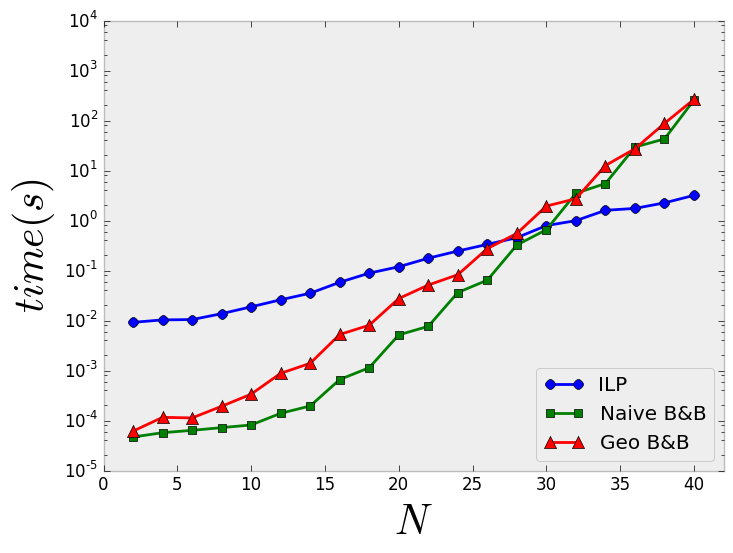
\includegraphics[width=0.9\linewidth]{Pictures/k1} 
		\caption{$K=0.25N$} 
		\label{fig:fixed_k:a} 
	\end{subfigure}%% 
	\begin{subfigure}[b]{0.4\linewidth}
		\centering
		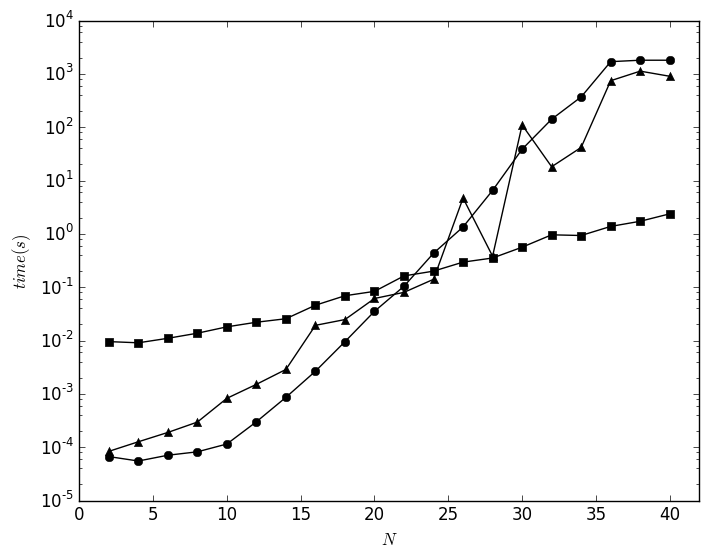
\includegraphics[width=0.9\linewidth]{Pictures/k2} 
		\caption{$K=0.5N$} 
		\label{fig:fixed_k:b} 
	\end{subfigure} 
	\begin{center}
	\begin{subfigure}[b]{0.4\linewidth}
		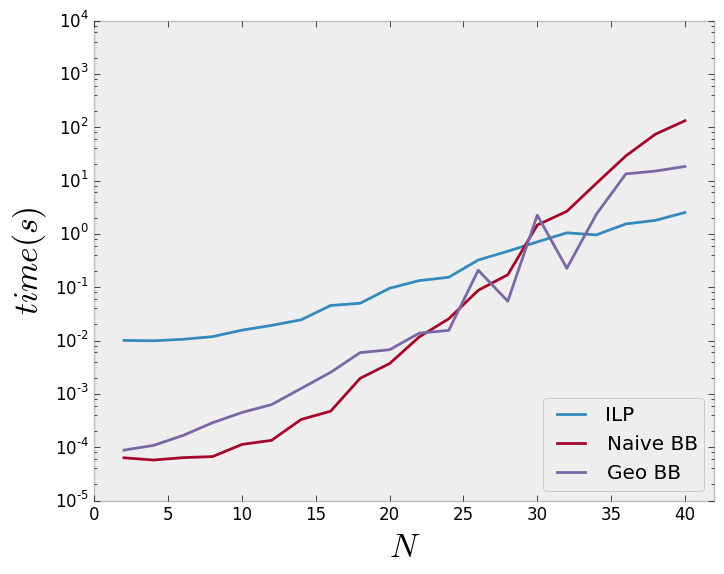
\includegraphics[width=0.9\linewidth]{Pictures/k3} 
		\caption{$K=0.75N$} 
		\label{fig:fixed_k:c} 
	\end{subfigure}
	\end{center}
	\begin{center}
    \textcolor{blue}{\cmark}\ -- Integer Linear Programming\quad   \textcolor{red}{\tmark}\ -- Delaunay Assisted B\&B\quad \textcolor{green}{\smark}\ -- Naive B\&B
    \end{center}
	\caption{CPU-time for different values of $K$ with varying values of $N$}
	\label{fig:fixed_k} 
\end{figure}


\noindent
As it can be seen, the problem solving time increases exponentially with the value of $N$, as expected.
The Integer Linear Programming Approach performs faster for larger values of $N$. Comparing the branch-and-bound approaches, these tests show that the Delaunay-assisted algorithm steadily approaches and surpasses the naïve branch-and-bound algorithm as the instance size grows.
\subsubsection*{Effect of $K$}
In this experiment, we analysed the performance of the three algorithms in dependence of parameter $K$. We fixed $N$ and varied $K$ from 2 to $N$ by steps of 2. Figure \cite{fig:fixed_n} show the results for the $N=\{10,20,30,40\}$, respectively. The tests were stopped at the half-hour mark. Figure \ref{fig:fixed_n} shows the results of these tests.
\begin{figure}[t] 
  \begin{subfigure}[b]{0.5\linewidth}
    \centering
    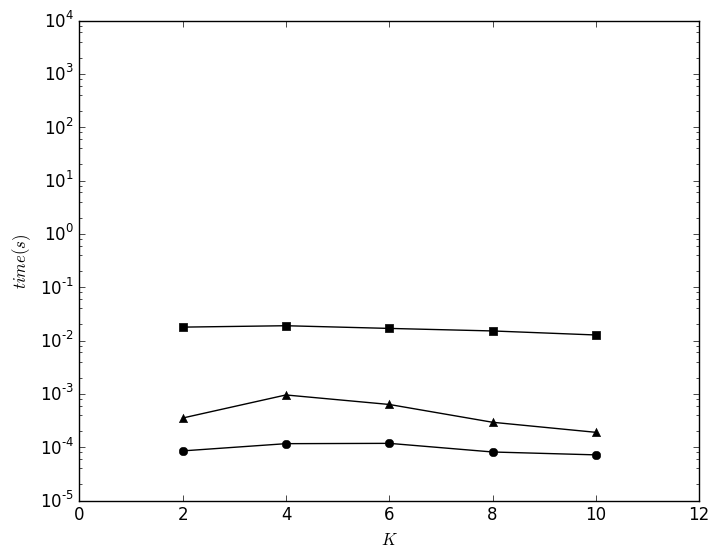
\includegraphics[width=0.9\linewidth]{Pictures/n10} 
    \caption{$N=10$} 
    \label{fig:fixed_n:a} 
    \vspace{4ex}
  \end{subfigure}%% 
  \begin{subfigure}[b]{0.5\linewidth}
    \centering
    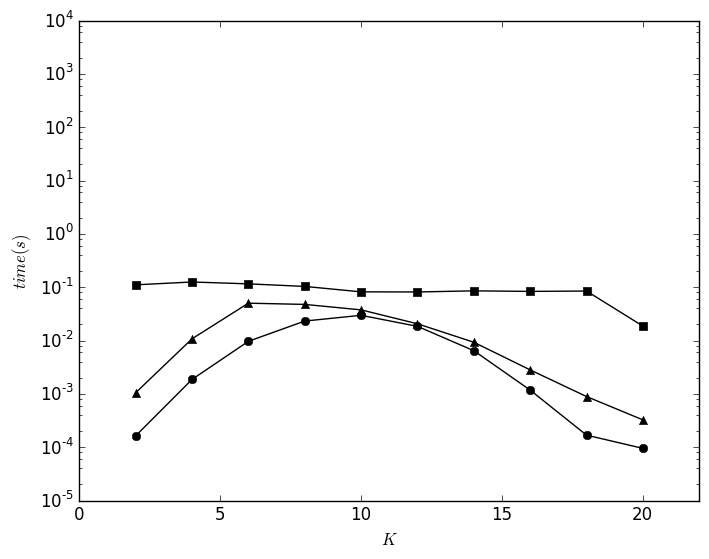
\includegraphics[width=0.9\linewidth]{Pictures/n20} 
    \caption{$N=20$} 
    \label{fig:fixed_n:b} 
    \vspace{4ex}
  \end{subfigure} 
  \begin{subfigure}[b]{0.5\linewidth}
    \centering
    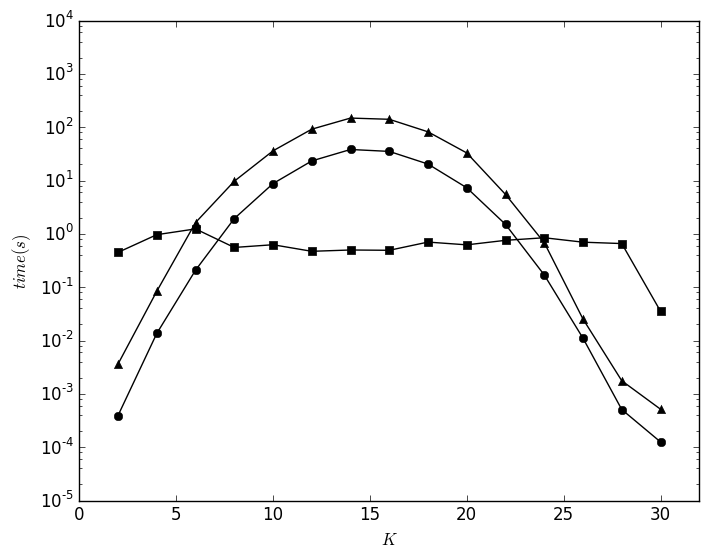
\includegraphics[width=0.9\linewidth]{Pictures/n30} 
    \caption{$N=30$} 
    \label{fig:fixed_n:c} 
  \end{subfigure}%%
  \begin{subfigure}[b]{0.5\linewidth}
    \centering
    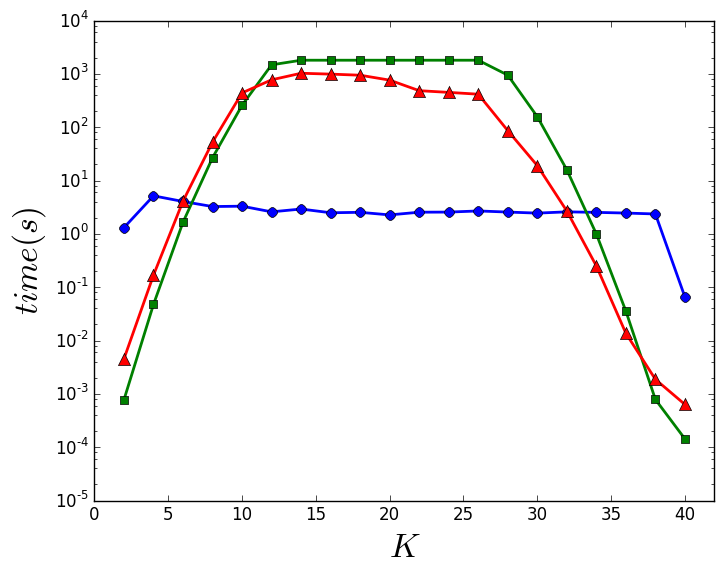
\includegraphics[width=0.9\linewidth]{Pictures/n40} 
    \caption{$N=40$} 
    \label{fig:fixed_n:d} 
  \end{subfigure} 
  \vspace{2ex}
  \begin{center}
  \textcolor{blue}{\cmark}\ -- Integer Linear Programming \quad   \textcolor{red}{\tmark}\ -- Delaunay Assisted B\&B\quad \textcolor{OliveGreen}{\smark}\ -- Naive B\&B
  \end{center}
  \caption{CPU-time for different values of $N$ with varying $K$}
  \label{fig:fixed_n} 
\end{figure}


\noindent
The Integer Linear Programming approach seems to be the fastest approach for most cases, and seems independent to the value of $K$. The exceptions to this seem to be smaller values of $N$, as well as the smallest and largest values of $K$. This happens because the implicit enumeration methods only need to enumerate a very small number of combinations.
As for the branch-and-bound algorithms, the Delaunay-assisted approach is slower than the Naïve implementation in these test cases. However it should be noted that for each $N$, the Delaunay-assisted algorithm peaks before the expected value of $K=N/2$. This is justified due to the fact that the Delaunay triangulation has an overhead which can take advantage for in larger values of $K$.
Furthermore, the fact that the Naïve implementation had no test for the middle values of $K$ for $N=40$ that ended before the time-out mark is noteworthy.
It is also worth noting that The Delaunay-assisted approach showed a lot more variance between tests, often taking much lower values than the mean. However, for the tests performed, two runs had values much larger than the Naïve approach, approximating the Delaunay-assisted algorithm's mean to the Naïve approach.

The time required for each test limited the number of tests performed. Because of this, the results may not be statistically meaningful. 
This could mean that the Delaunay-assisted approach is only preferable for values of $N$ and $K$ to which neither approach is usable in real-time. Due to the small number of tests for large values of $N$, this result may not be statistically meaningful, but it is noteworthy.

\section{Discussion}
The algorithms in this chapter have some drawbacks when used in a web application. Not only were the running times too large to be used in real-time, taking minutes and even hours for small instances with 40 points at most, but they also required some a priori knowledge about the number of clusters on a given window. This is infeasible, since there is no efficient way to infer how many clusters there are in a new region, without testing for all possible values of $K$. The algorithm should be able to calculate the final number of selected points, constrained to a minimum distance factor between them. This can be achieved by solving \emph{Geometric Disk Cover} problem described in Section \ref{ilp2}. The next chapter describes in detail a way to solve this problem in regards to the final application.

\cleardoublepage
\chapter{Geometric Disk Cover}
\label{chap:approx}
%\lhead{Chapter \ref{chap:approx}. \emph{\nameref{chap:approx}}} % This is for the header

The goal of the geometric disk cover problem is to, given a set $N$ of points and a minimum distance $d$, find the smallest number $k$ of circles of radius $d$ centred around points in $N$ such that no point is left uncovered. This chapter describes an efficient way to approximate the optimal solution to this new problem. The number of points selected by the algorithm is bound above by $m \ln {n}$ points, where $m$ is the optimal value of $k$.

\section{Approximation Algorithm}
Calculating the optimal solution for Geometric Disk Cover is a \emph{NP-hard} problem \cite{gdccomplex}. However, there are ways of finding a reasonable approximation to the optimal solution in a short amount of time. Briefly, this approach requires two steps. The first step is the Proximity Graph Building step, which builds a graph connecting all pairs of points that are close together. The second step is a Set Cover step, which uses an approximation algorithm to cover the graph built in the former step. The following sections describe these steps in more detail.

\subsection{Proximity Graph Construction}
The first step is to create a graph connecting all pairs points that are within a distance of each other. This means constructing a graph in which every point is a vertex, and every edge connects two vertices whose points are within the given distance, also known as a proximity graph \cite{proximity}. The naïve approach to building this graph would be to test all the distances between each pair of points, taking $\bigo(n^2)$ operations. Alternatively a line sweep algorithm or a series of range searches on a \kdtree could be used to speed up the process. The line sweep algorithm would require a $\bigo(n \log{n})$ sorting algorithm, followed by $\bigo(n^2)$ comparisons. However, the latter is limited by the number of points within the sliding window, which should only contain a fraction of the total number of points on the map, since the distance chosen is a fraction of its dimensions. The \kdtree range search, on the other hand, requires a $\bigo(n \log{n})$ construction of a \kdtree using a median of medians algorithm. This is followed by $n$ queries consisting of finding the points within a square of side $2d$ centred around each of the points. Each one of these operations take $\bigo(\sqrt{N}+m)$ time, where $m$ is the number of returned points \cite{kdrange}. Even though the complexity of the \kdtree range search is theoretically faster than the line sweep method, it comes with an extra overhead of handling a more complex structure. As such, both methods are analysed from an experimental point of view in this thesis. After this operation, the graph connecting all neighbours is built. Figure \ref{fig:aa1} illustrates one such graph.

\begin{figure}[H]
	\begin{center}
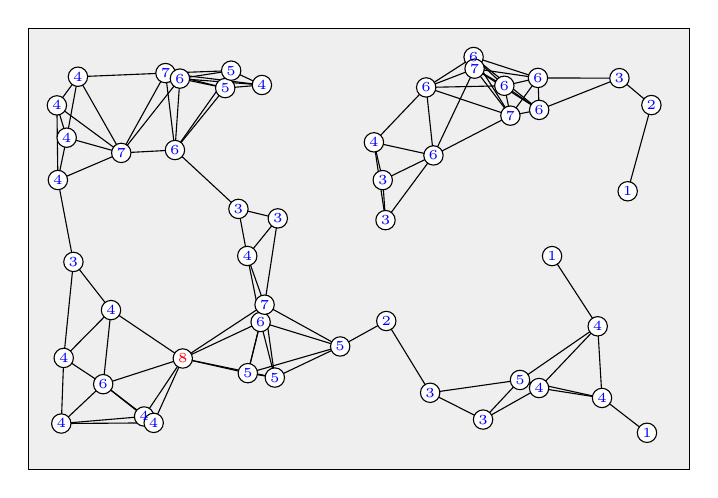
\begin{tikzpicture}[scale=1.4]
\fill[lightgray!25,draw=black] (0,0) rectangle (6,4);
\clip (0,0) rectangle (6,4);-
\draw [](0.26,3.3) -- (0.269,2.623);
\draw [](0.26,3.3) -- (0.349,3.007);
\draw [](0.26,3.3) -- (0.451,3.56);
\draw [](0.26,3.3) -- (0.844,2.869);
\draw [](0.269,2.623) -- (0.349,3.007);
\draw [](0.269,2.623) -- (0.41,1.88);
\draw [](0.269,2.623) -- (0.844,2.869);
\draw [](0.3,0.414) -- (0.322,1.009);
\draw [](0.3,0.414) -- (0.68,0.771);
\draw [](0.3,0.414) -- (1.051,0.478);
\draw [](0.3,0.414) -- (1.138,0.42);
\draw [](0.322,1.009) -- (0.41,1.88);
\draw [](0.322,1.009) -- (0.68,0.771);
\draw [](0.322,1.009) -- (0.751,1.443);
\draw [](0.349,3.007) -- (0.451,3.56);
\draw [](0.349,3.007) -- (0.844,2.869);
\draw [](0.41,1.88) -- (0.751,1.443);
\draw [](0.451,3.56) -- (0.844,2.869);
\draw [](0.451,3.56) -- (1.245,3.593);
\draw [](0.68,0.771) -- (0.751,1.443);
\draw [](0.68,0.771) -- (1.051,0.478);
\draw [](0.68,0.771) -- (1.138,0.42);
\draw [](0.68,0.771) -- (1.402,1.004);
\draw [](0.751,1.443) -- (1.402,1.004);
\draw [](0.844,2.869) -- (1.245,3.593);
\draw [](0.844,2.869) -- (1.331,2.895);
\draw [](0.844,2.869) -- (1.376,3.543);
\draw [](1.051,0.478) -- (1.138,0.42);
\draw [](1.051,0.478) -- (1.402,1.004);
\draw [](1.138,0.42) -- (1.402,1.004);
\draw [](1.245,3.593) -- (1.331,2.895);
\draw [](1.245,3.593) -- (1.376,3.543);
\draw [](1.245,3.593) -- (1.787,3.457);
\draw [](1.245,3.593) -- (1.841,3.615);
\draw [](1.245,3.593) -- (2.12,3.485);
\draw [](1.331,2.895) -- (1.376,3.543);
\draw [](1.331,2.895) -- (1.787,3.457);
\draw [](1.331,2.895) -- (1.841,3.615);
\draw [](1.331,2.895) -- (1.907,2.361);
\draw [](1.376,3.543) -- (1.787,3.457);
\draw [](1.376,3.543) -- (1.841,3.615);
\draw [](1.376,3.543) -- (2.12,3.485);
\draw [](1.402,1.004) -- (1.992,0.871);
\draw [](1.402,1.004) -- (2.108,1.335);
\draw [](1.402,1.004) -- (2.144,1.492);
\draw [](1.402,1.004) -- (2.237,0.831);
\draw [](1.787,3.457) -- (1.841,3.615);
\draw [](1.787,3.457) -- (2.12,3.485);
\draw [](1.841,3.615) -- (2.12,3.485);
\draw [](1.907,2.361) -- (1.987,1.934);
\draw [](1.907,2.361) -- (2.264,2.275);
\draw [](1.987,1.934) -- (2.108,1.335);
\draw [](1.987,1.934) -- (2.144,1.492);
\draw [](1.987,1.934) -- (2.264,2.275);
\draw [](1.992,0.871) -- (2.108,1.335);
\draw [](1.992,0.871) -- (2.144,1.492);
\draw [](1.992,0.871) -- (2.237,0.831);
\draw [](1.992,0.871) -- (2.83,1.113);
\draw [](2.108,1.335) -- (2.144,1.492);
\draw [](2.108,1.335) -- (2.237,0.831);
\draw [](2.108,1.335) -- (2.83,1.113);
\draw [](2.144,1.492) -- (2.237,0.831);
\draw [](2.144,1.492) -- (2.264,2.275);
\draw [](2.144,1.492) -- (2.83,1.113);
\draw [](2.237,0.831) -- (2.83,1.113);
\draw [](2.83,1.113) -- (3.248,1.344);
\draw [](3.136,2.965) -- (3.216,2.622);
\draw [](3.136,2.965) -- (3.241,2.259);
\draw [](3.136,2.965) -- (3.61,3.463);
\draw [](3.136,2.965) -- (3.676,2.846);
\draw [](3.216,2.622) -- (3.241,2.259);
\draw [](3.216,2.622) -- (3.676,2.846);
\draw [](3.241,2.259) -- (3.676,2.846);
\draw [](3.248,1.344) -- (3.646,0.693);
\draw [](3.61,3.463) -- (3.676,2.846);
\draw [](3.61,3.463) -- (4.04,3.739);
\draw [](3.61,3.463) -- (4.049,3.633);
\draw [](3.61,3.463) -- (4.319,3.478);
\draw [](3.61,3.463) -- (4.374,3.207);
\draw [](3.646,0.693) -- (4.126,0.45);
\draw [](3.646,0.693) -- (4.461,0.809);
\draw [](3.676,2.846) -- (4.049,3.633);
\draw [](3.676,2.846) -- (4.374,3.207);
\draw [](4.04,3.739) -- (4.049,3.633);
\draw [](4.04,3.739) -- (4.319,3.478);
\draw [](4.04,3.739) -- (4.374,3.207);
\draw [](4.04,3.739) -- (4.624,3.549);
\draw [](4.04,3.739) -- (4.635,3.259);
\draw [](4.049,3.633) -- (4.319,3.478);
\draw [](4.049,3.633) -- (4.374,3.207);
\draw [](4.049,3.633) -- (4.624,3.549);
\draw [](4.049,3.633) -- (4.635,3.259);
\draw [](4.126,0.45) -- (4.461,0.809);
\draw [](4.126,0.45) -- (4.634,0.736);
\draw [](4.319,3.478) -- (4.374,3.207);
\draw [](4.319,3.478) -- (4.624,3.549);
\draw [](4.319,3.478) -- (4.635,3.259);
\draw [](4.374,3.207) -- (4.624,3.549);
\draw [](4.374,3.207) -- (4.635,3.259);
\draw [](4.461,0.809) -- (4.634,0.736);
\draw [](4.461,0.809) -- (5.166,1.296);
\draw [](4.461,0.809) -- (5.205,0.646);
\draw [](4.624,3.549) -- (4.635,3.259);
\draw [](4.624,3.549) -- (5.363,3.547);
\draw [](4.634,0.736) -- (5.166,1.296);
\draw [](4.634,0.736) -- (5.205,0.646);
\draw [](4.635,3.259) -- (5.363,3.547);
\draw [](4.752,1.933) -- (5.166,1.296);
\draw [](5.166,1.296) -- (5.205,0.646);
\draw [](5.205,0.646) -- (5.613,0.33);
\draw [](5.363,3.547) -- (5.653,3.303);
\draw [](5.438,2.521) -- (5.653,3.303);
\fill [white,draw=black] (0.26,3.3) circle (2.5pt);
\fill [white,draw=black] (0.269,2.623) circle (2.5pt);
\fill [white,draw=black] (0.3,0.414) circle (2.5pt);
\fill [white,draw=black] (0.322,1.009) circle (2.5pt);
\fill [white,draw=black] (0.349,3.007) circle (2.5pt);
\fill [white,draw=black] (0.41,1.88) circle (2.5pt);
\fill [white,draw=black] (0.451,3.56) circle (2.5pt);
\fill [white,draw=black] (0.68,0.771) circle (2.5pt);
\fill [white,draw=black] (0.751,1.443) circle (2.5pt);
\fill [white,draw=black] (0.844,2.869) circle (2.5pt);
\fill [white,draw=black] (1.051,0.478) circle (2.5pt);
\fill [white,draw=black] (1.138,0.42) circle (2.5pt);
\fill [white,draw=black] (1.245,3.593) circle (2.5pt);
\fill [white,draw=black] (1.331,2.895) circle (2.5pt);
\fill [white,draw=black] (1.376,3.543) circle (2.5pt);
\fill [white,draw=black] (1.402,1.004) circle (2.5pt);
\fill [white,draw=black] (1.787,3.457) circle (2.5pt);
\fill [white,draw=black] (1.841,3.615) circle (2.5pt);
\fill [white,draw=black] (1.907,2.361) circle (2.5pt);
\fill [white,draw=black] (1.987,1.934) circle (2.5pt);
\fill [white,draw=black] (1.992,0.871) circle (2.5pt);
\fill [white,draw=black] (2.108,1.335) circle (2.5pt);
\fill [white,draw=black] (2.12,3.485) circle (2.5pt);
\fill [white,draw=black] (2.144,1.492) circle (2.5pt);
\fill [white,draw=black] (2.237,0.831) circle (2.5pt);
\fill [white,draw=black] (2.264,2.275) circle (2.5pt);
\fill [white,draw=black] (2.83,1.113) circle (2.5pt);
\fill [white,draw=black] (3.136,2.965) circle (2.5pt);
\fill [white,draw=black] (3.216,2.622) circle (2.5pt);
\fill [white,draw=black] (3.241,2.259) circle (2.5pt);
\fill [white,draw=black] (3.248,1.344) circle (2.5pt);
\fill [white,draw=black] (3.61,3.463) circle (2.5pt);
\fill [white,draw=black] (3.646,0.693) circle (2.5pt);
\fill [white,draw=black] (3.676,2.846) circle (2.5pt);
\fill [white,draw=black] (4.04,3.739) circle (2.5pt);
\fill [white,draw=black] (4.049,3.633) circle (2.5pt);
\fill [white,draw=black] (4.126,0.45) circle (2.5pt);
\fill [white,draw=black] (4.319,3.478) circle (2.5pt);
\fill [white,draw=black] (4.374,3.207) circle (2.5pt);
\fill [white,draw=black] (4.461,0.809) circle (2.5pt);
\fill [white,draw=black] (4.624,3.549) circle (2.5pt);
\fill [white,draw=black] (4.634,0.736) circle (2.5pt);
\fill [white,draw=black] (4.635,3.259) circle (2.5pt);
\fill [white,draw=black] (4.752,1.933) circle (2.5pt);
\fill [white,draw=black] (5.166,1.296) circle (2.5pt);
\fill [white,draw=black] (5.205,0.646) circle (2.5pt);
\fill [white,draw=black] (5.363,3.547) circle (2.5pt);
\fill [white,draw=black] (5.438,2.521) circle (2.5pt);
\fill [white,draw=black] (5.613,0.33) circle (2.5pt);
\fill [white,draw=black] (5.653,3.303) circle (2.5pt);
\node [blue] at (0.26,3.3) {\tiny $4$};
\node [blue] at (0.269,2.623) {\tiny $4$};
\node [blue] at (0.3,0.414) {\tiny $4$};
\node [blue] at (0.322,1.009) {\tiny $4$};
\node [blue] at (0.349,3.007) {\tiny $4$};
\node [blue] at (0.41,1.88) {\tiny $3$};
\node [blue] at (0.451,3.56) {\tiny $4$};
\node [blue] at (0.68,0.771) {\tiny $6$};
\node [blue] at (0.751,1.443) {\tiny $4$};
\node [blue] at (0.844,2.869) {\tiny $7$};
\node [blue] at (1.051,0.478) {\tiny $4$};
\node [blue] at (1.138,0.42) {\tiny $4$};
\node [blue] at (1.245,3.593) {\tiny $7$};
\node [blue] at (1.331,2.895) {\tiny $6$};
\node [blue] at (1.376,3.543) {\tiny $6$};
\node [red] at (1.402,1.004) {\tiny $8$};
\node [blue] at (1.787,3.457) {\tiny $5$};
\node [blue] at (1.841,3.615) {\tiny $5$};
\node [blue] at (1.907,2.361) {\tiny $3$};
\node [blue] at (1.987,1.934) {\tiny $4$};
\node [blue] at (1.992,0.871) {\tiny $5$};
\node [blue] at (2.108,1.335) {\tiny $6$};
\node [blue] at (2.12,3.485) {\tiny $4$};
\node [blue] at (2.144,1.492) {\tiny $7$};
\node [blue] at (2.237,0.831) {\tiny $5$};
\node [blue] at (2.264,2.275) {\tiny $3$};
\node [blue] at (2.83,1.113) {\tiny $5$};
\node [blue] at (3.136,2.965) {\tiny $4$};
\node [blue] at (3.216,2.622) {\tiny $3$};
\node [blue] at (3.241,2.259) {\tiny $3$};
\node [blue] at (3.248,1.344) {\tiny $2$};
\node [blue] at (3.61,3.463) {\tiny $6$};
\node [blue] at (3.646,0.693) {\tiny $3$};
\node [blue] at (3.676,2.846) {\tiny $6$};
\node [blue] at (4.04,3.739) {\tiny $6$};
\node [blue] at (4.049,3.633) {\tiny $7$};
\node [blue] at (4.126,0.45) {\tiny $3$};
\node [blue] at (4.319,3.478) {\tiny $6$};
\node [blue] at (4.374,3.207) {\tiny $7$};
\node [blue] at (4.461,0.809) {\tiny $5$};
\node [blue] at (4.624,3.549) {\tiny $6$};
\node [blue] at (4.634,0.736) {\tiny $4$};
\node [blue] at (4.635,3.259) {\tiny $6$};
\node [blue] at (4.752,1.933) {\tiny $1$};
\node [blue] at (5.166,1.296) {\tiny $4$};
\node [blue] at (5.205,0.646) {\tiny $4$};
\node [blue] at (5.363,3.547) {\tiny $3$};
\node [blue] at (5.438,2.521) {\tiny $1$};
\node [blue] at (5.613,0.33) {\tiny $1$};
\node [blue] at (5.653,3.303) {\tiny $2$};
\end{tikzpicture}

\end{center}
\caption{Illustration of the Resulting Graph. The numbers on the points represent the number of neighbours. The number in red represents the point with the largest number of neighbours.}
\label{fig:aa1}
\end{figure}


This graph is represented via adjacency lists. The adjacency lists have an advantage over an adjacency matrix as linked lists can be used to considerably reduce the memory footprint in sparse graphs. It also allows for faster sequential access to the neighbours of any given point. These linked lists share similarities to the half-edge structure, in which each node represents a unidirectional edge that contains a pointer to its counterpart.

It is noteworthy that the graph can reach $\bigo(n^2)$ edges if the points are all very close together and/or the minimum distance is large enough. This case coupled with the fact that the adjacency linked lists occupy more space per edge than an adjacency matrix, the space needed to keep the graph in memory can be potentially too high for some machines to handle larger instances of the problem. 

\subsection{Set Cover}
The second step to the algorithm is to chose a small subset of vertices whose neighbours unions are equal to the whole set of graph's vertices. This is known as \emph{set cover}, and its solution can be approximated using a greedy approach \cite{approxalgos}. Starting with the whole uncovered graph, the point with the largest number of uncovered neighbours is selected. This is done iteratively until no uncovered points remain on the graph. This approach approximates the number of points to within $m \ln{n}$ points, were $m$ is the optimal number.

At each step of this algorithm, one point $p$ and all its neighbours and respective edges must be removed from the graph. This is done by iterating through the adjacency lists of the neighbours of $p$ and deleting all the connections to their neighbours (second-degree neighbours of $p$). This operation takes exactly $\bigo(n)$ time where $n$ is proportional to the number of edges to be deleted. Figure \ref{fig:aa2} illustrates the graph after the first iteration:

\begin{figure}[H]
\begin{center}
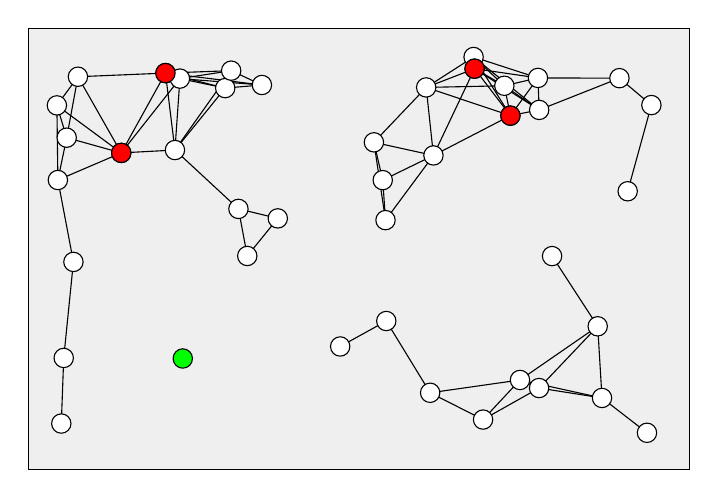
\begin{tikzpicture}[scale=1.4]
\fill[lightgray!25,draw=black] (0,0) rectangle (6,4);
\clip (0,0) rectangle (6,4);
\draw [](0.26,3.3) -- (0.269,2.623);
\draw [](0.26,3.3) -- (0.349,3.007);
\draw [](0.26,3.3) -- (0.451,3.56);
\draw [](0.26,3.3) -- (0.844,2.869);
\draw [](0.269,2.623) -- (0.349,3.007);
\draw [](0.269,2.623) -- (0.41,1.88);
\draw [](0.269,2.623) -- (0.844,2.869);
\draw [](0.3,0.414) -- (0.322,1.009);
\draw [](0.322,1.009) -- (0.41,1.88);
\draw [](0.349,3.007) -- (0.451,3.56);
\draw [](0.349,3.007) -- (0.844,2.869);
\draw [](0.451,3.56) -- (0.844,2.869);
\draw [](0.451,3.56) -- (1.245,3.593);
\draw [](0.844,2.869) -- (1.245,3.593);
\draw [](0.844,2.869) -- (1.331,2.895);
\draw [](0.844,2.869) -- (1.376,3.543);
\draw [](1.245,3.593) -- (1.331,2.895);
\draw [](1.245,3.593) -- (1.376,3.543);
\draw [](1.245,3.593) -- (1.787,3.457);
\draw [](1.245,3.593) -- (1.841,3.615);
\draw [](1.245,3.593) -- (2.12,3.485);
\draw [](1.331,2.895) -- (1.376,3.543);
\draw [](1.331,2.895) -- (1.787,3.457);
\draw [](1.331,2.895) -- (1.841,3.615);
\draw [](1.331,2.895) -- (1.907,2.361);
\draw [](1.376,3.543) -- (1.787,3.457);
\draw [](1.376,3.543) -- (1.841,3.615);
\draw [](1.376,3.543) -- (2.12,3.485);
\draw [](1.787,3.457) -- (1.841,3.615);
\draw [](1.787,3.457) -- (2.12,3.485);
\draw [](1.841,3.615) -- (2.12,3.485);
\draw [](1.907,2.361) -- (1.987,1.934);
\draw [](1.907,2.361) -- (2.264,2.275);
\draw [](1.987,1.934) -- (2.264,2.275);
\draw [](2.83,1.113) -- (3.248,1.344);
\draw [](3.136,2.965) -- (3.216,2.622);
\draw [](3.136,2.965) -- (3.241,2.259);
\draw [](3.136,2.965) -- (3.61,3.463);
\draw [](3.136,2.965) -- (3.676,2.846);
\draw [](3.216,2.622) -- (3.241,2.259);
\draw [](3.216,2.622) -- (3.676,2.846);
\draw [](3.241,2.259) -- (3.676,2.846);
\draw [](3.248,1.344) -- (3.646,0.693);
\draw [](3.61,3.463) -- (3.676,2.846);
\draw [](3.61,3.463) -- (4.04,3.739);
\draw [](3.61,3.463) -- (4.049,3.633);
\draw [](3.61,3.463) -- (4.319,3.478);
\draw [](3.61,3.463) -- (4.374,3.207);
\draw [](3.646,0.693) -- (4.126,0.45);
\draw [](3.646,0.693) -- (4.461,0.809);
\draw [](3.676,2.846) -- (4.049,3.633);
\draw [](3.676,2.846) -- (4.374,3.207);
\draw [](4.04,3.739) -- (4.049,3.633);
\draw [](4.04,3.739) -- (4.319,3.478);
\draw [](4.04,3.739) -- (4.374,3.207);
\draw [](4.04,3.739) -- (4.624,3.549);
\draw [](4.04,3.739) -- (4.635,3.259);
\draw [](4.049,3.633) -- (4.319,3.478);
\draw [](4.049,3.633) -- (4.374,3.207);
\draw [](4.049,3.633) -- (4.624,3.549);
\draw [](4.049,3.633) -- (4.635,3.259);
\draw [](4.126,0.45) -- (4.461,0.809);
\draw [](4.126,0.45) -- (4.634,0.736);
\draw [](4.319,3.478) -- (4.374,3.207);
\draw [](4.319,3.478) -- (4.624,3.549);
\draw [](4.319,3.478) -- (4.635,3.259);
\draw [](4.374,3.207) -- (4.624,3.549);
\draw [](4.374,3.207) -- (4.635,3.259);
\draw [](4.461,0.809) -- (4.634,0.736);
\draw [](4.461,0.809) -- (5.166,1.296);
\draw [](4.461,0.809) -- (5.205,0.646);
\draw [](4.624,3.549) -- (4.635,3.259);
\draw [](4.624,3.549) -- (5.363,3.547);
\draw [](4.634,0.736) -- (5.166,1.296);
\draw [](4.634,0.736) -- (5.205,0.646);
\draw [](4.635,3.259) -- (5.363,3.547);
\draw [](4.752,1.933) -- (5.166,1.296);
\draw [](5.166,1.296) -- (5.205,0.646);
\draw [](5.205,0.646) -- (5.613,0.33);
\draw [](5.363,3.547) -- (5.653,3.303);
\draw [](5.438,2.521) -- (5.653,3.303);
\fill [white,draw=black] (0.26,3.3) circle (2.5pt);
\fill [white,draw=black] (0.269,2.623) circle (2.5pt);
\fill [white,draw=black] (0.3,0.414) circle (2.5pt);
\fill [white,draw=black] (0.322,1.009) circle (2.5pt);
\fill [white,draw=black] (0.349,3.007) circle (2.5pt);
\fill [white,draw=black] (0.41,1.88) circle (2.5pt);
\fill [white,draw=black] (0.451,3.56) circle (2.5pt);
\fill [white,draw=black] (0.844,2.869) circle (2.5pt);
\fill [white,draw=black] (1.245,3.593) circle (2.5pt);
\fill [white,draw=black] (1.331,2.895) circle (2.5pt);
\fill [white,draw=black] (1.376,3.543) circle (2.5pt);
\fill [white,draw=black] (1.787,3.457) circle (2.5pt);
\fill [white,draw=black] (1.841,3.615) circle (2.5pt);
\fill [white,draw=black] (1.907,2.361) circle (2.5pt);
\fill [white,draw=black] (1.987,1.934) circle (2.5pt);
\fill [white,draw=black] (2.12,3.485) circle (2.5pt);
\fill [white,draw=black] (2.264,2.275) circle (2.5pt);
\fill [white,draw=black] (2.83,1.113) circle (2.5pt);
\fill [white,draw=black] (3.136,2.965) circle (2.5pt);
\fill [white,draw=black] (3.216,2.622) circle (2.5pt);
\fill [white,draw=black] (3.241,2.259) circle (2.5pt);
\fill [white,draw=black] (3.248,1.344) circle (2.5pt);
\fill [white,draw=black] (3.61,3.463) circle (2.5pt);
\fill [white,draw=black] (3.646,0.693) circle (2.5pt);
\fill [white,draw=black] (3.676,2.846) circle (2.5pt);
\fill [white,draw=black] (4.04,3.739) circle (2.5pt);
\fill [white,draw=black] (4.049,3.633) circle (2.5pt);
\fill [white,draw=black] (4.126,0.45) circle (2.5pt);
\fill [white,draw=black] (4.319,3.478) circle (2.5pt);
\fill [white,draw=black] (4.374,3.207) circle (2.5pt);
\fill [white,draw=black] (4.461,0.809) circle (2.5pt);
\fill [white,draw=black] (4.624,3.549) circle (2.5pt);
\fill [white,draw=black] (4.634,0.736) circle (2.5pt);
\fill [white,draw=black] (4.635,3.259) circle (2.5pt);
\fill [white,draw=black] (4.752,1.933) circle (2.5pt);
\fill [white,draw=black] (5.166,1.296) circle (2.5pt);
\fill [white,draw=black] (5.205,0.646) circle (2.5pt);
\fill [white,draw=black] (5.363,3.547) circle (2.5pt);
\fill [white,draw=black] (5.438,2.521) circle (2.5pt);
\fill [white,draw=black] (5.613,0.33) circle (2.5pt);
\fill [white,draw=black] (5.653,3.303) circle (2.5pt);
%\node [blue] at (0.26,3.3) {\tiny $4$};
%\node [blue] at (0.269,2.623) {\tiny $4$};
%\node [blue] at (0.3,0.414) {\tiny $1$};
%\node [blue] at (0.322,1.009) {\tiny $2$};
%\node [blue] at (0.349,3.007) {\tiny $4$};
%\node [blue] at (0.41,1.88) {\tiny $2$};
%\node [blue] at (0.451,3.56) {\tiny $4$};
%\node [red] at (0.844,2.869) {\tiny $7$};
%\node [red] at (1.245,3.593) {\tiny $7$};
%\node [blue] at (1.331,2.895) {\tiny $6$};
%\node [blue] at (1.376,3.543) {\tiny $6$};
%\node [blue] at (1.787,3.457) {\tiny $5$};
%\node [blue] at (1.841,3.615) {\tiny $5$};
%\node [blue] at (1.907,2.361) {\tiny $3$};
%\node [blue] at (1.987,1.934) {\tiny $2$};
%\node [blue] at (2.12,3.485) {\tiny $4$};
%\node [blue] at (2.264,2.275) {\tiny $2$};
%\node [blue] at (2.83,1.113) {\tiny $1$};
%\node [blue] at (3.136,2.965) {\tiny $4$};
%\node [blue] at (3.216,2.622) {\tiny $3$};
%\node [blue] at (3.241,2.259) {\tiny $3$};
%\node [blue] at (3.248,1.344) {\tiny $2$};
%\node [blue] at (3.61,3.463) {\tiny $6$};
%\node [blue] at (3.646,0.693) {\tiny $3$};
%\node [blue] at (3.676,2.846) {\tiny $6$};
%\node [blue] at (4.04,3.739) {\tiny $6$};
%\node [red] at (4.049,3.633) {\tiny $7$};
%\node [blue] at (4.126,0.45) {\tiny $3$};
%\node [blue] at (4.319,3.478) {\tiny $6$};
%\node [red] at (4.374,3.207) {\tiny $7$};
%\node [blue] at (4.461,0.809) {\tiny $5$};
%\node [blue] at (4.624,3.549) {\tiny $6$};
%\node [blue] at (4.634,0.736) {\tiny $4$};
%\node [blue] at (4.635,3.259) {\tiny $6$};
%\node [blue] at (4.752,1.933) {\tiny $1$};
%\node [blue] at (5.166,1.296) {\tiny $4$};
%\node [blue] at (5.205,0.646) {\tiny $4$};
%\node [blue] at (5.363,3.547) {\tiny $3$};
%\node [blue] at (5.438,2.521) {\tiny $1$};
%\node [blue] at (5.613,0.33) {\tiny $1$};
%\node [blue] at (5.653,3.303) {\tiny $2$};
\fill [red,draw=black] (0.844,2.869) circle (2.5pt);
%\node [red] at (0.844,2.869) {\tiny $7$};
\fill [red,draw=black] (1.245,3.593) circle (2.5pt);
%\node [red] at (1.245,3.593) {\tiny $7$};
\fill [red,draw=black] (4.049,3.633) circle (2.5pt);
%\node [red] at (4.049,3.633) {\tiny $7$};
\fill [red,draw=black] (4.374,3.207) circle (2.5pt);
%\node [red] at (4.374,3.207) {\tiny $7$};
\fill [green,draw=black] (1.402,1.004) circle (2.5pt);
\end{tikzpicture}

\end{center}
\caption{Illustration of the state of the graph after the first iteration. Any of the red points is to be removed in the next iteration, as they have the largest amount of neighbours.}
\label{fig:aa2}
\end{figure}


After all the points are covered, the collection of selected centres makes the subset of centroids that is displayed as the final output. The cardinality of this set does not exceed the approximation as described above.

\begin{figure}[H]
\begin{center}
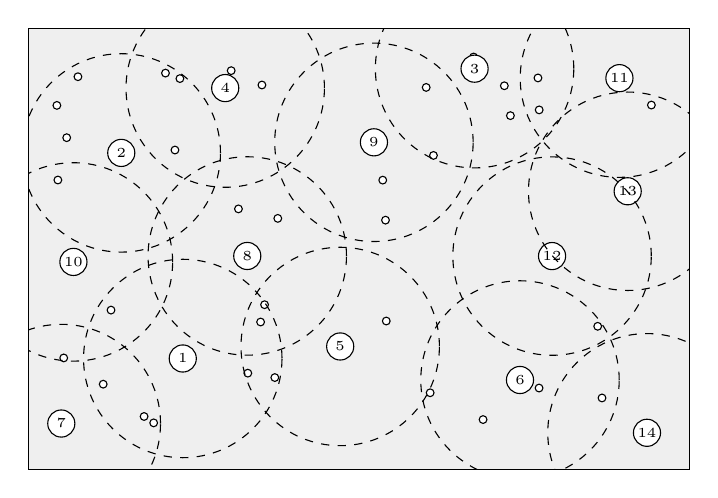
\begin{tikzpicture}[scale=1.4]
\fill[lightgray!25,draw=black] (0,0) rectangle (6,4);
\clip (0,0) rectangle (6,4);


\fill [white,draw=black] (0.26,3.3) circle (1pt);
\fill [white,draw=black] (0.269,2.623) circle (1pt);
\fill [white,draw=black] (0.3,0.414) circle (1pt);
\fill [white,draw=black] (0.322,1.009) circle (1pt);
\fill [white,draw=black] (0.349,3.007) circle (1pt);
\fill [white,draw=black] (0.41,1.88) circle (1pt);
\fill [white,draw=black] (0.451,3.56) circle (1pt);
\fill [white,draw=black] (0.68,0.771) circle (1pt);
\fill [white,draw=black] (0.751,1.443) circle (1pt);
\fill [white,draw=black] (0.844,2.869) circle (1pt);
\fill [white,draw=black] (1.051,0.478) circle (1pt);
\fill [white,draw=black] (1.138,0.42) circle (1pt);
\fill [white,draw=black] (1.245,3.593) circle (1pt);
\fill [white,draw=black] (1.331,2.895) circle (1pt);
\fill [white,draw=black] (1.376,3.543) circle (1pt);
\fill [white,draw=black] (1.402,1.004) circle (1pt);
\fill [white,draw=black] (1.787,3.457) circle (1pt);
\fill [white,draw=black] (1.841,3.615) circle (1pt);
\fill [white,draw=black] (1.907,2.361) circle (1pt);
\fill [white,draw=black] (1.987,1.934) circle (1pt);
\fill [white,draw=black] (1.992,0.871) circle (1pt);
\fill [white,draw=black] (2.108,1.335) circle (1pt);
\fill [white,draw=black] (2.12,3.485) circle (1pt);
\fill [white,draw=black] (2.144,1.492) circle (1pt);
\fill [white,draw=black] (2.237,0.831) circle (1pt);
\fill [white,draw=black] (2.264,2.275) circle (1pt);
\fill [white,draw=black] (2.83,1.113) circle (1pt);
\fill [white,draw=black] (3.136,2.965) circle (1pt);
\fill [white,draw=black] (3.216,2.622) circle (1pt);
\fill [white,draw=black] (3.241,2.259) circle (1pt);
\fill [white,draw=black] (3.248,1.344) circle (1pt);
\fill [white,draw=black] (3.61,3.463) circle (1pt);
\fill [white,draw=black] (3.646,0.693) circle (1pt);
\fill [white,draw=black] (3.676,2.846) circle (1pt);
\fill [white,draw=black] (4.04,3.739) circle (1pt);
\fill [white,draw=black] (4.049,3.633) circle (1pt);
\fill [white,draw=black] (4.126,0.45) circle (1pt);
\fill [white,draw=black] (4.319,3.478) circle (1pt);
\fill [white,draw=black] (4.374,3.207) circle (1pt);
\fill [white,draw=black] (4.461,0.809) circle (1pt);
\fill [white,draw=black] (4.624,3.549) circle (1pt);
\fill [white,draw=black] (4.634,0.736) circle (1pt);
\fill [white,draw=black] (4.635,3.259) circle (1pt);
\fill [white,draw=black] (4.752,1.933) circle (1pt);
\fill [white,draw=black] (5.166,1.296) circle (1pt);
\fill [white,draw=black] (5.205,0.646) circle (1pt);
\fill [white,draw=black] (5.363,3.547) circle (1pt);
\fill [white,draw=black] (5.438,2.521) circle (1pt);
\fill [white,draw=black] (5.613,0.33) circle (1pt);
\fill [white,draw=black] (5.653,3.303) circle (1pt);


\fill [white,draw=black] (1.402,1.004) circle (3.5pt);
\node [black] at (1.402,1.004) {\tiny $1$};
\fill [white,draw=black] (0.844,2.869) circle (3.5pt);
\node [black] at (0.844,2.869) {\tiny $2$};
\fill [white,draw=black] (4.049,3.633) circle (3.5pt);
\node [black] at (4.049,3.633) {\tiny $3$};
\fill [white,draw=black] (1.787,3.457) circle (3.5pt);
\node [black] at (1.787,3.457) {\tiny $4$};
\fill [white,draw=black] (2.83,1.113) circle (3.5pt);
\node [black] at (2.83,1.113) {\tiny $5$};
\fill [white,draw=black] (4.461,0.809) circle (3.5pt);
\node [black] at (4.461,0.809) {\tiny $6$};
\fill [white,draw=black] (0.3,0.414) circle (3.5pt);
\node [black] at (0.3,0.414) {\tiny $7$};
\fill [white,draw=black] (1.987,1.934) circle (3.5pt);
\node [black] at (1.987,1.934) {\tiny $8$};
\fill [white,draw=black] (3.136,2.965) circle (3.5pt);
\node [black] at (3.136,2.965) {\tiny $9$};
\fill [white,draw=black] (0.41,1.88) circle (3.5pt);
\node [black] at (0.41,1.88) {\tiny $10$};
\fill [white,draw=black] (5.363,3.547) circle (3.5pt);
\node [black] at (5.363,3.547) {\tiny $11$};
\fill [white,draw=black] (4.752,1.933) circle (3.5pt);
\node [black] at (4.752,1.933) {\tiny $12$};
\fill [white,draw=black] (5.438,2.521) circle (3.5pt);
\node [black] at (5.438,2.521) {\tiny $13$};
\fill [white,draw=black] (5.613,0.33) circle (3.5pt);
\node [black] at (5.613,0.33) {\tiny $14$};
\draw [dashed] (1.402,1.004) circle (0.9);
\draw [dashed] (0.844,2.869) circle (0.9);
\draw [dashed] (4.049,3.633) circle (0.9);
\draw [dashed] (1.787,3.457) circle (0.9);
\draw [dashed] (2.83,1.113) circle (0.9);
\draw [dashed] (4.461,0.809) circle (0.9);
\draw [dashed] (0.3,0.414) circle (0.9);
\draw [dashed] (1.987,1.934) circle (0.9);
\draw [dashed] (3.136,2.965) circle (0.9);
\draw [dashed] (0.41,1.88) circle (0.9);
\draw [dashed] (5.363,3.547) circle (0.9);
\draw [dashed] (4.752,1.933) circle (0.9);
\draw [dashed] (5.438,2.521) circle (0.9);
\draw [dashed] (5.613,0.33) circle (0.9);

\end{tikzpicture}

\end{center}
\caption{Illustration of the state of the final chosen set. The larger points are the chosen set, and the numbers represent the order in which they are chosen.}
\label{fig:aa3}


\end{figure}

\subsection{Results}
\begin{change}
This section reports both approaches (\kdtrees and line sweeping) to the graph building portion of the algorithm. Only the proximity graph building half of the algorithms is implemented in more than one way. This is because the set cover half has a much more efficient algorithm, time complexity wise. In fact, running a code profiler shows that the graph building stage takes 98\% of the CPU-time, with the time taken to run the set cover algorithm stage being negligible.
\end{change}

For the tests in this section, the given value of $d$ is the minimum distance between points, therefore radius of the covering disks. It is given as a percentage of the largest dimension of the window, as this value is easier to adjust and analyse by a human user.
Figure \ref{fig:sweden_dist} shows the outputs for different values of $d$ for a set of points of interest in Sweden.

\begin{figure}[!h] 
  \begin{subfigure}[b]{0.24\linewidth}
		\centering
		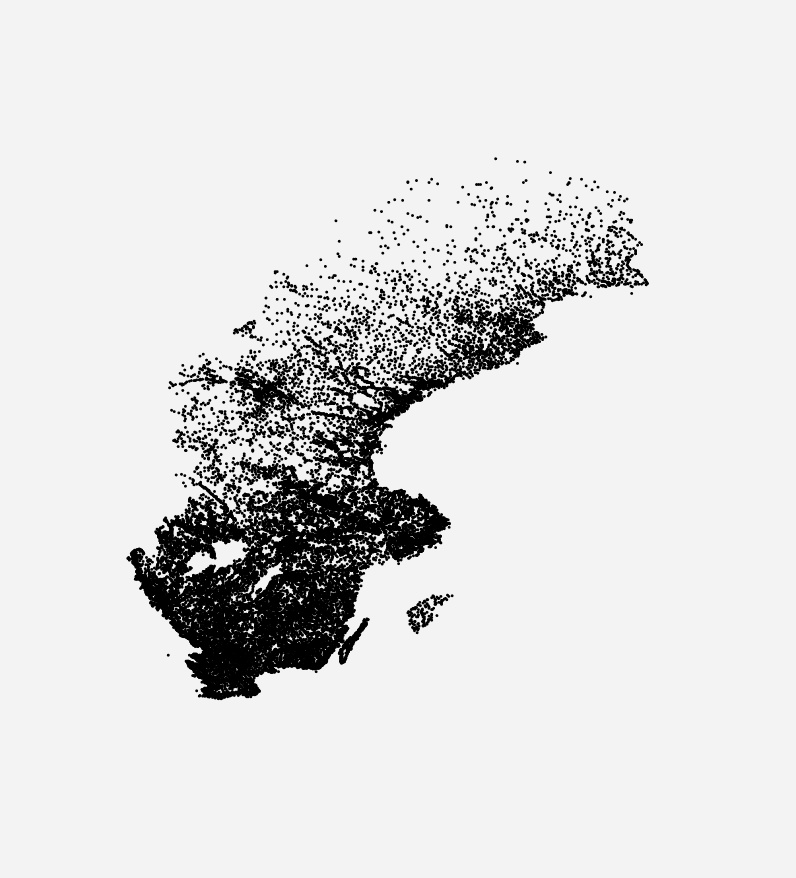
\includegraphics[width=0.9\linewidth]{Pictures/sweden} 
		\caption{\small Original Set} 
		\label{fig:or_sweden} 
		\vspace{4ex}
  \end{subfigure}
  \begin{subfigure}[b]{0.24\linewidth}
    \centering
    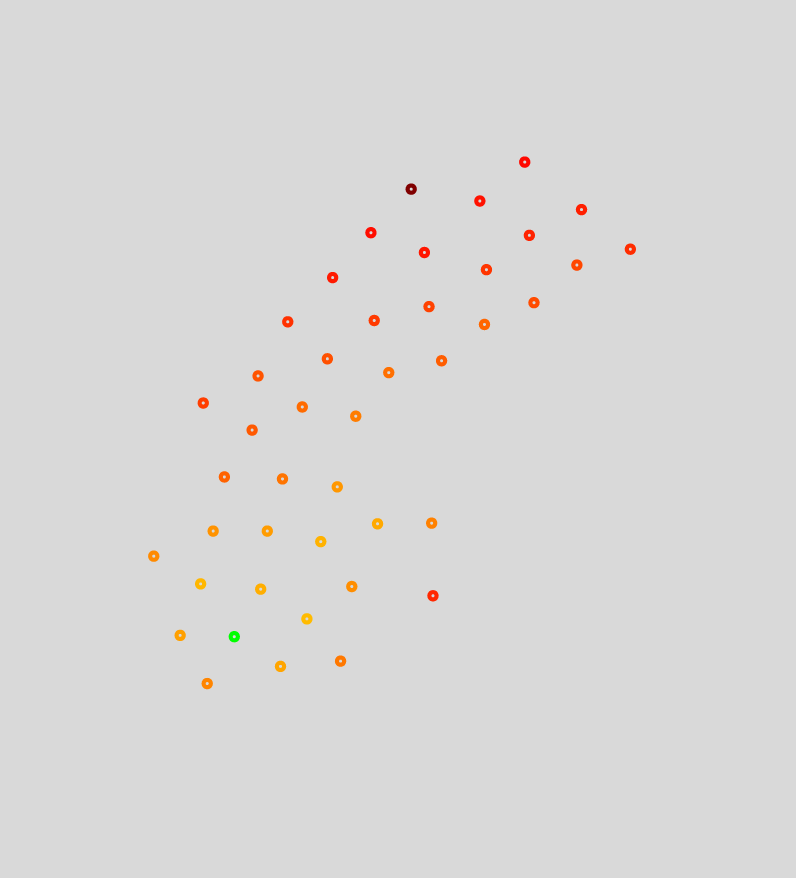
\includegraphics[width=0.9\linewidth]{Pictures/10_sweden} 
	\caption{\small $d=10\%$} 
    \label{fig:10_sweden} 
    \vspace{4ex}
  \end{subfigure}%% 
  \begin{subfigure}[b]{0.24\linewidth}
    \centering
    
\includegraphics[width=0.9\linewidth]{Pictures/15_sweden} 
    \caption{\small $d=15\%$} 
    \label{fig:15_sweden} 
    \vspace{4ex}
  \end{subfigure}
  \begin{subfigure}[b]{0.24\linewidth}
  	\centering
  	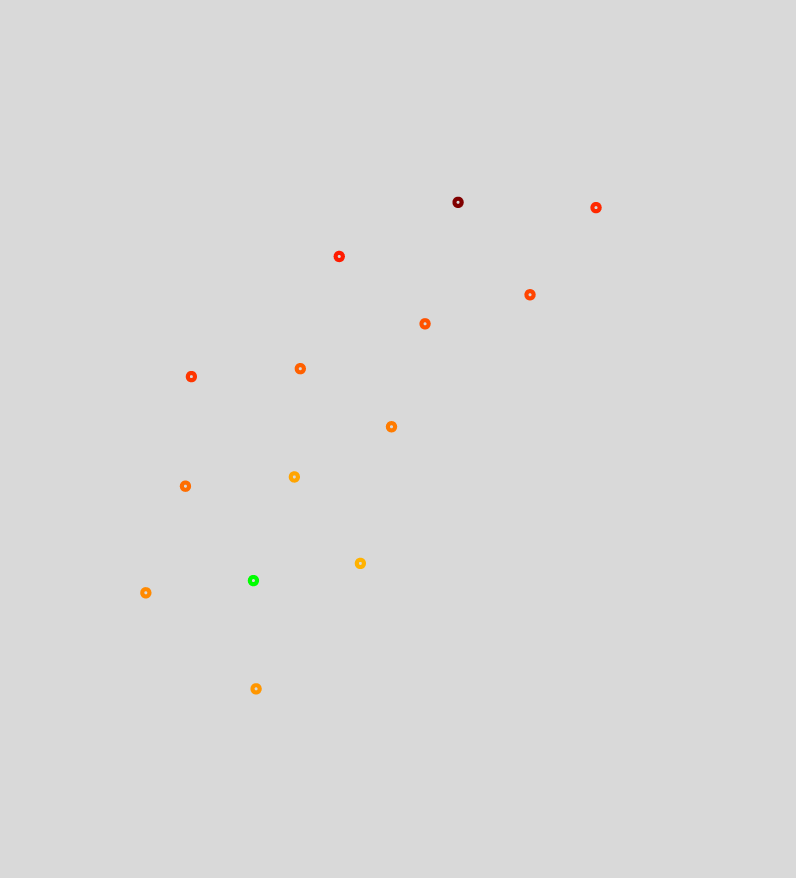
\includegraphics[width=0.9\linewidth]{Pictures/20_sweden} 
  	\caption{\small $d=20\%$} 
  	\label{fig:20_sweden} 
  	\vspace{4ex}
  \end{subfigure}
  \caption[Selected subsets from both graph building algorithms]{Selected subsets from both graph building algorithms.}
  \label{fig:sweden_dist} 
\end{figure}


\begin{change}
By analysing images of a few real-world examples, the values for the minimum distance $d$ were agreed to be given as a value between 10\% and 15\% of the largest dimension of the window. These values give the subsets that were deemed as the easiest to look at without losing sense of shape of the area. The performance tests still use the value of 20\% to test the algorithms under less favourable conditions, since the larger the value of $d$, the denser and more time is required to build the proximity graph. 
\end{change}

Since the algorithms in this chapter are more efficient than the ones in the previous chapter, new tests were needed to benchmark them. These tests use random inputs to benchmark the performance of the algorithms. Both uniform and clustered inputs are tested. The uniform inputs are a simple collection of $N$ points whose Cartesian coordinates are randomly chosen between $0$ and $100$. The clustered inputs are generated by choosing a random number of points $s$ between 10 to 20 points. Each of these points acts as a centre and is chosen by randomly generating two Cartesian coordinates between 0 and 100. Around each of these, $N/s$ points were generated by randomly choosing an angle $\Theta$ (between $0$ and $2\pi$) and a distance $\rho$ (between $10$ and $20$), which represent the polar coordinates around their respective central point. These tests generate circular clusters, with more density towards the centre.

Each test is performed 30 times, with shared seeds between the algorithms. The times listed do include the input scanning. All algorithms are implemented using ANSI C89 and compiled using \emph{gcc 5.1.0}. The programs were ran on a machine with a Intel i7 Dual-Core, 2GHz processor, with a 8 GB, 1600 MHz memory and Arch Linux 3.14.4 x64 as its operating system.

The first test performed benchmarked both line sweep and \kdtree range search algorithms for the proximity graph construction. The results are shown in Figure \ref{fig:ls_kd_t}.

\begin{figure}[!h] 
	\centering
    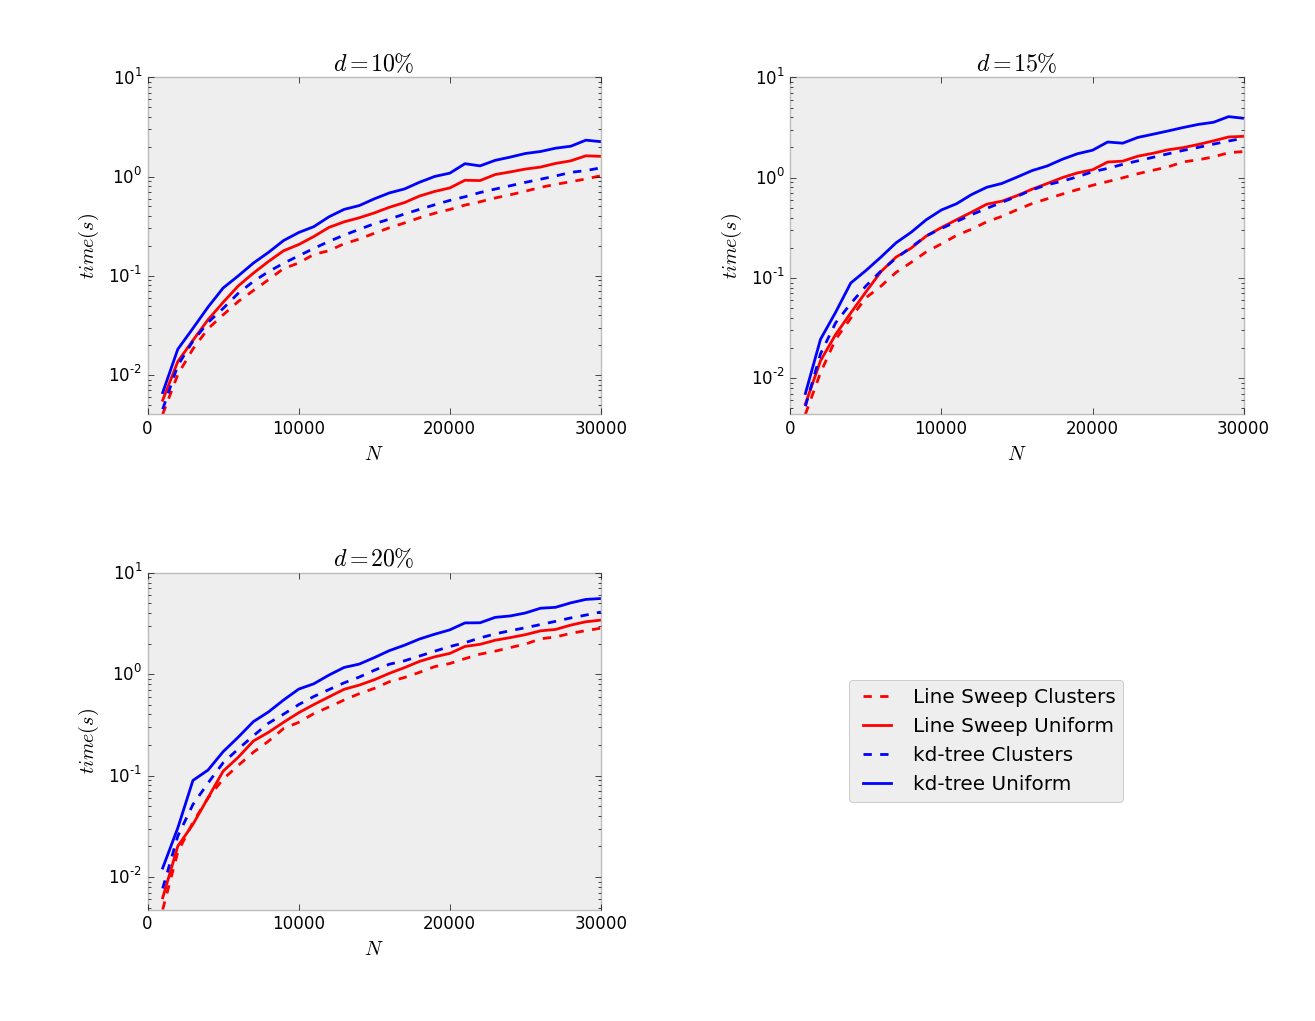
\includegraphics[width=\linewidth]{Pictures/ls_kd_t}
    \caption[CPU-time for Line Sweep and $k$-d Tree range search.]{CPU-time for both proximity graph algorithms on uniform and clustered inputs for different values of $d$.}
    \label{fig:ls_kd_t} 
\end{figure}



As Figure \ref{fig:ls_kd_t} shows, the line sweep method performs faster in both the uniform and the clustered data. The lower expected complexity of the \kdtrees does not compensate the larger overhead in their construction. It can also be seen that both algorithms become slower the larger the number of points, as was expected. It should be noted that the algorithm is very memory intensive. Even with adjacency lists instead of a matrix, the inputs can generate a instance where every point must be connected to every other point. In this case, the advantage of the adjacency lists for sparse graphs is lost, and the program exceeds the RAM limit given by the Operating system. This occurs more frequently for larger values of $d$, and $N$, with the smallest case recorded being of $N=25000$ and $d=0.2$ on a clustered input that generated most clusters on top of each other, concentrating most points within a circle of a small radius, where most of them had over 20000 neighbours. 

Applying both methods to any given case gives similar results. The coverage algorithm picks the points with most neighbours. Since two different points may have the same number of neighbours, and the two algorithms sort the points in two different ways, there may occur a case where the sets are completely different, based on which point is select first in case of a draw. The values still fall bellow the upper bound for the approximation factor, and no algorithm should have the advantage. Figure \ref{fig:ls_kd_k} shows the number of points selected by each algorithm in the same instances as above.

\begin{figure}[H] 
  \begin{subfigure}[b]{0.5\linewidth}
    \centering
    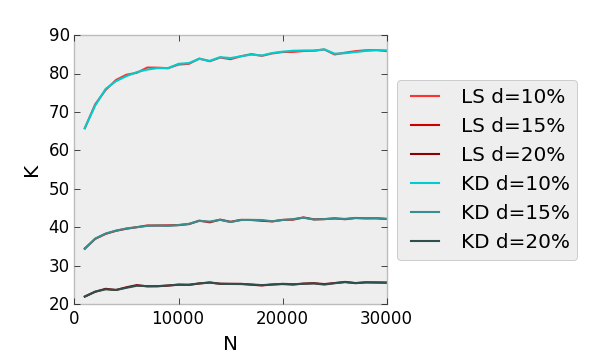
\includegraphics[width=0.9\linewidth]{Pictures/unif_kd_ls_k} 
    %\caption{$N=10$} 
    \label{fig:unif_kd_ls_k} 
    \vspace{4ex}
  \end{subfigure}%% 
  \begin{subfigure}[b]{0.5\linewidth}
    \centering
    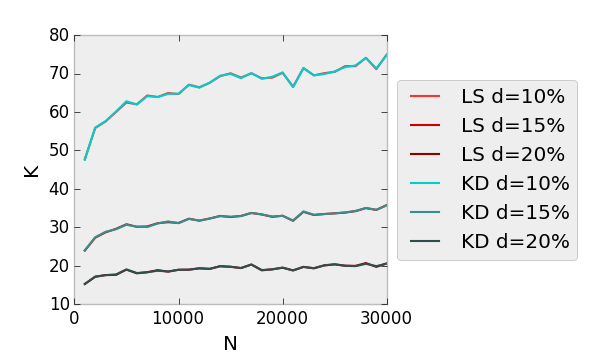
\includegraphics[width=0.9\linewidth]{Pictures/clus_kd_ls_k} 
    %\caption{$N=20$} 
    \label{fig:clus_kd_ls_k} 
    \vspace{4ex}
  \end{subfigure}
  \caption[Number $K$ of points selected for Line Sweep and $k$-d Tree range search]{Number $K$ of points selected for both proximity graph algorithms on uniform inputs(left) and clustered inputs(right).}
  \label{fig:kd_ls_k} 
\end{figure}




\begin{change}
Figure \ref{fig:ls_kd_k} shows  that the number of selected points does not seem to change for the same values of $d$. In fact, the growth of the value of $k$ seems to suggest an asymptotic approach to a fixed value. This happens because there is a limit to how many circles can be placed in an area without any of them containing the centres of the others. 
	
The process of finding the best disposition of circles of the same radius in a given area is known as circle packing. The number of circles in a circle packing instance for a square area is given by the ratio between the circles' radii and the width of the square enclosing them. Since the value for $d$ is given as a fraction of the size of the window, the bound values of $k$ can be calculated for the various values of $d$. A detailed explanation of how to calculate these values is given in Appendix \ref{ann:packing}. The values indicate that $k$ should not be larger than $\{128,59,36\}$, for the given values $d=\{0.1,0.15,0.2\}$, respectively. With the exception of the latter, these values are yet to be proven to be optimal, but are not expected to be very different, and serve as a good estimate of the maximum number of points that can be selected.
\end{change}

Figure \ref{fig:ls_kd_k} also shows that no algorithm has the advantage on the number of points chosen. In fact, the results overlap each other almost completely. This suggests that the best algorithm to use is the line sweep algorithm, as it takes less time to compute similar results.


\section{Heuristic Speed-ups}
The approximation algorithm runs rather efficiently, taking under 1 second for 30000 points for the uniform inputs, and under 3 seconds for the clustered inputs. This result can be improved by employing some heuristic filtering methods to the inputs. However, by using these approaches, the guarantee of the quality is lost. Nevertheless, the results mean that the algorithm should be considered to handle larger numbers of points.
\subsection{Sampling}
The simplest method to accelerating the algorithms is to simply ignore a random set of those points. With the smaller sample of points, the algorithm should run faster. If the points are removed uniformly, then the shape should still be kept.

Figure \ref{fig:ls_rs_t} shows the time difference between the regular line sweep and the sampled input.

\begin{figure}[H] 
	\centering
	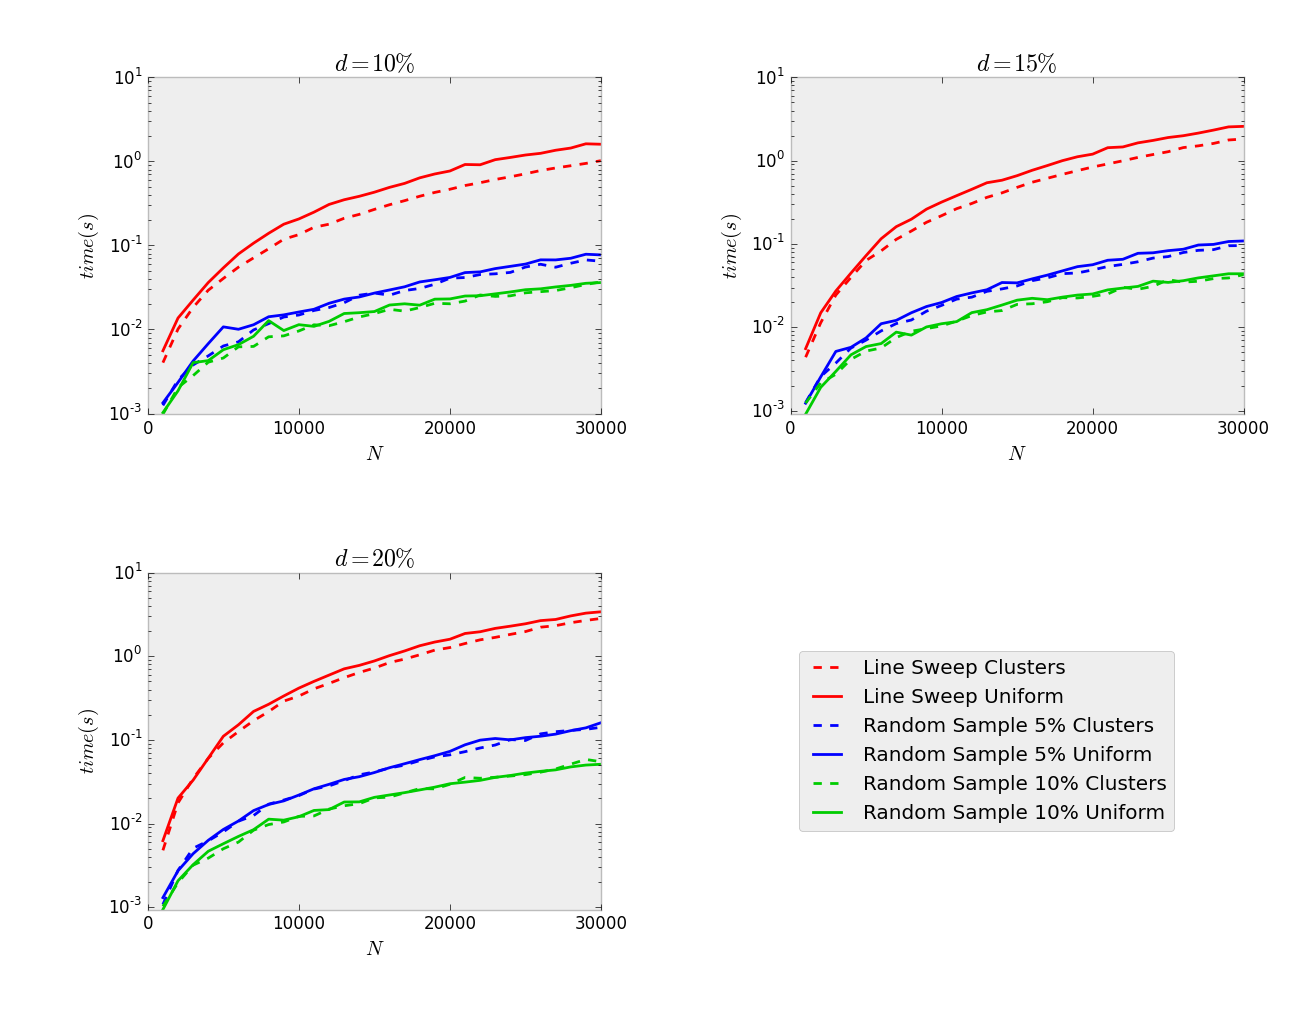
\includegraphics[width=0.8\linewidth]{Pictures/ls_rs_t} 
	\caption[CPU-time for Line Sweep and Random Sampling algorithms.]{CPU-time for the line sweep algorithm, and two instances of the random sampling, with 5\% and 10\% of the total points, for different values of $d$.}
	\label{fig:ls_rs_t} 
\end{figure}

The graph in Figure \ref{fig:ls_rs_t} proves that the sampling is indeed faster, no cases exceeded the memory limit. However, upon closer inspection, it can be noted that the result is not optimal. Figure \ref{fig:ls_rs_k} shows that the number of selected points is inferior:

\begin{figure}[H] 
  \begin{subfigure}[b]{0.5\linewidth}
    \centering
    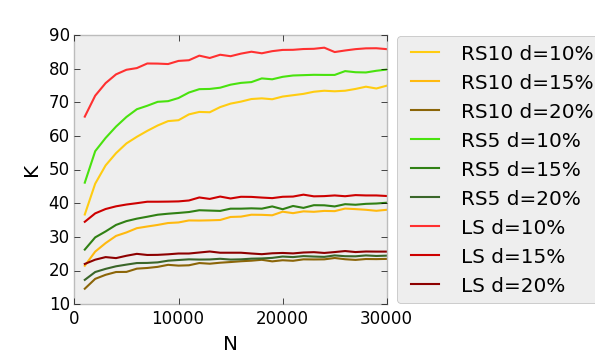
\includegraphics[width=0.9\linewidth]{Pictures/unif_ls_rs_k} 
    %\caption{$N=10$} 
    \label{fig:unif_ls_rs_k} 
    \vspace{4ex}
  \end{subfigure}%% 
  \begin{subfigure}[b]{0.5\linewidth}
    \centering
    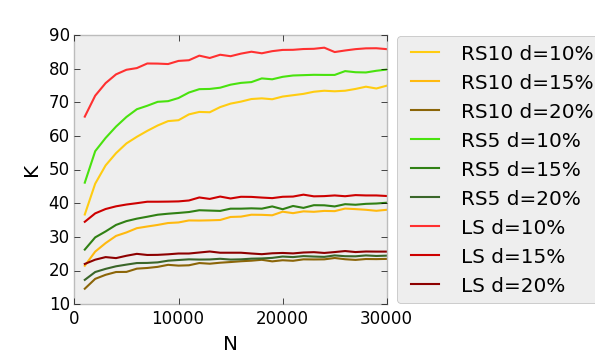
\includegraphics[width=0.9\linewidth]{Pictures/unif_ls_rs_k} 
    %\caption{$N=20$} 
    \label{fig:clus_ls_rs_k} 
    \vspace{4ex}
  \end{subfigure}
  \caption{Number $K$ of points selected for both random sample algorithms on uniform points(left) and clustered points (right). The red lines represent the control group (line sweep), the green lines represent the 1/5th sampling and the yellow lines represent the 1/10th sampling}
  \label{fig:ls_rs_k} 
\end{figure}



This can be explained by the fact that the algorithm is not accounting for all points. In fact, the number of cases where a point is left isolated in the full set algorithms is decreased by the factor of the sampling in these algorithms. This means that not all points are being covered, and the number of selected points decreases. Figure \ref{fig:ls_rs_greece} shows this effect in a real map:

\begin{figure}[!h] 
  \centering
  \begin{subfigure}[b]{0.45\linewidth}
    \centering
    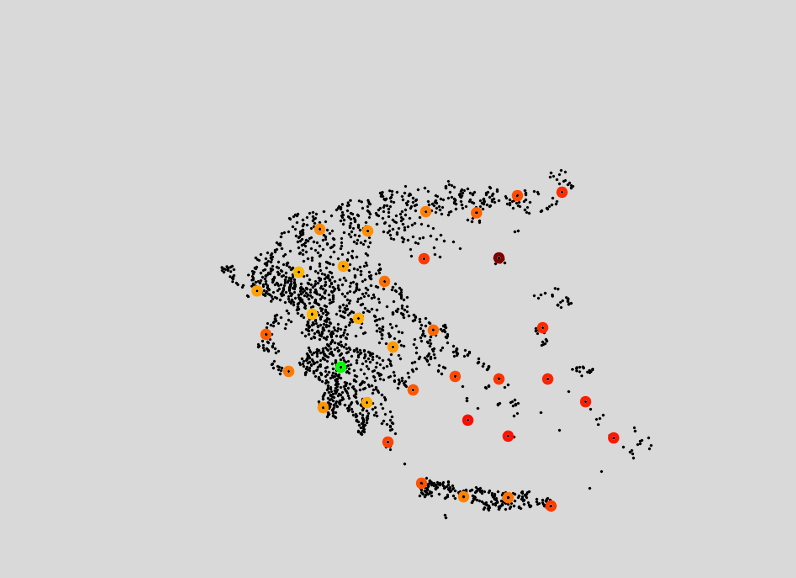
\includegraphics[width=0.9\linewidth]{Pictures/rs_greece} 
    %\caption{$N=10$} 
    \label{fig:ls_greece} 
  \end{subfigure}%% 
  \begin{subfigure}[b]{0.45\linewidth}
    \centering
    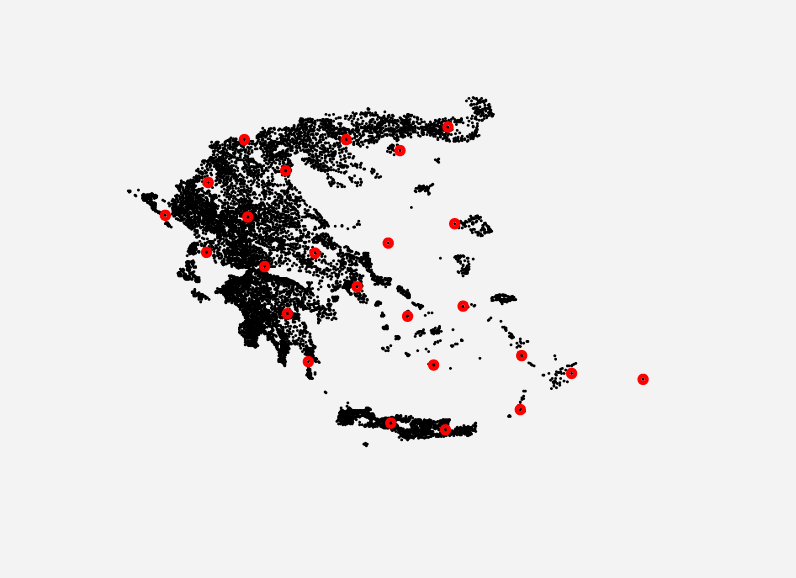
\includegraphics[width=0.9\linewidth]{Pictures/ls_greece} 
    %\caption{$N=20$} 
    \label{fig:rs_greece} 
  \end{subfigure}
  \label{fig:ls_rs_greece} 
\end{figure}



As shown, the sampled subset does not cover the most isolated points. In fact, the westernmost point in the map is not present in the sample and, therefore, is not covered. This method is not suitable for the initial requirements, since very isolated points have only a small chance of being represented.

\subsection{Two-phase filtering}
A solution to the random sampling algorithm problems is to perform two passes of the approximation algorithm for the geometric disk cover problem. The first pass over the points is done with a very small radius. This can be done very quickly, since the range search only has to look in a very small area. Using a small distance speeds the algorithm up, as seen in Figure \ref{fig:ls_rs_t}. This means that many of the points that are close to each other are discarded, but a representative neighbour is left in its place. Isolated points are not discarded. The resulting set is much smaller than the original, whilst still keeping a representativeness degree. The second pass, with the final intended distance now takes advantage of the much smaller set of points for the speed up. The \emph{CPU} times for two instances of the algorithm can be seen in Figure \ref{fig:ls_bp_t}. The values of the first pass distance $d^\prime$ are given as a percentage of the final pass distance $d$. One of the instances uses $d^\prime=5\%d$, another $d^\prime=10\%d$ and the other uses $d^\prime=20\%d$.

\begin{figure}[!h]  
	\vspace{-25pt}
	\centering
	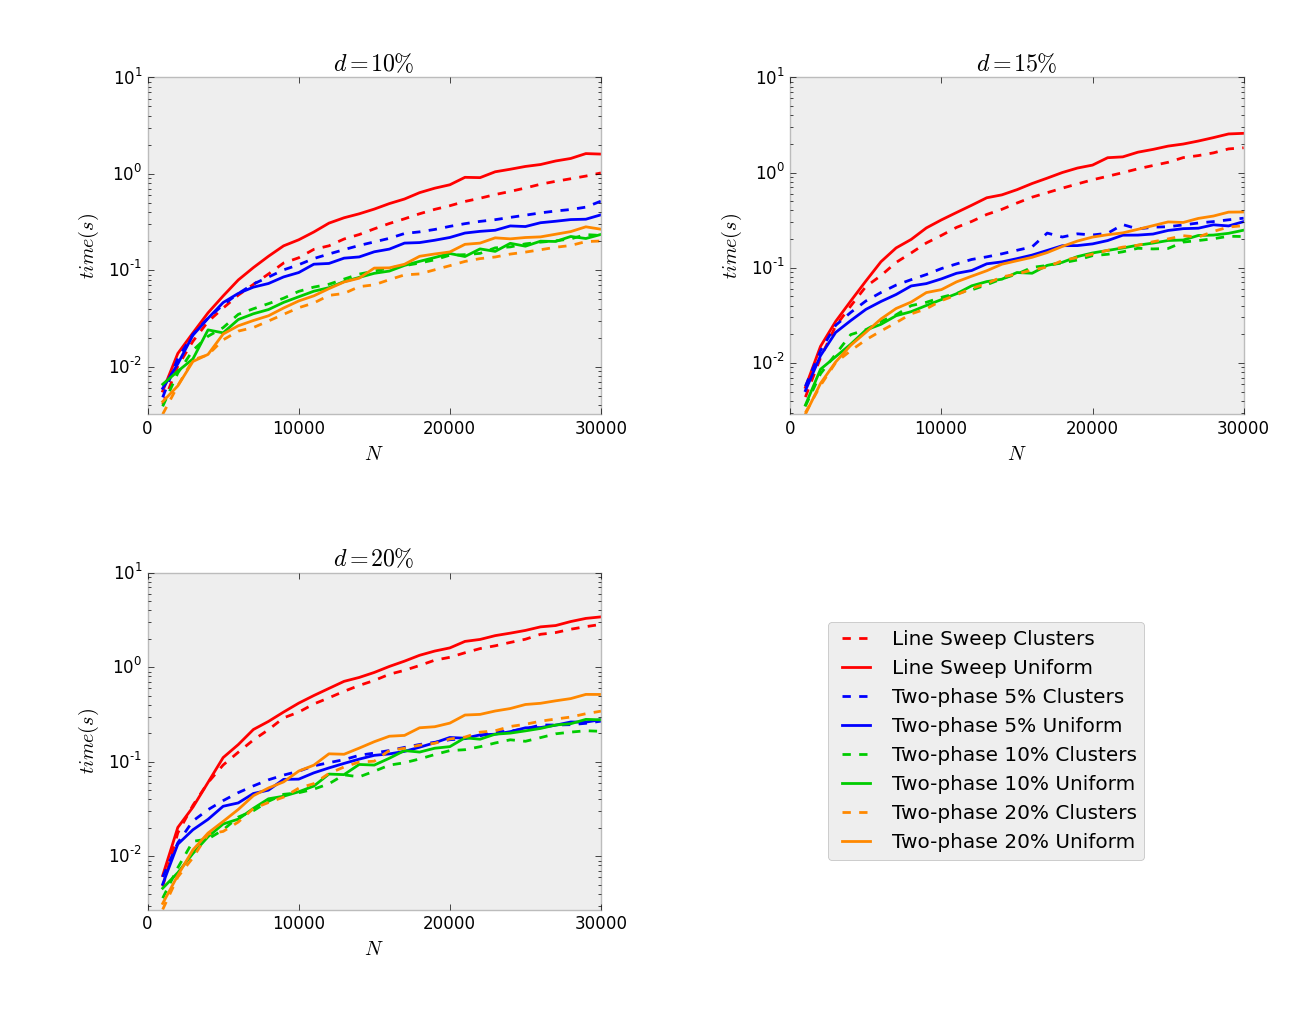
\includegraphics[width=\linewidth]{Pictures/ls_bp_t} 
	\label{fig:ls_bp_t} 
\end{figure}

As it can be seen, the two-phase filtering is very fast and does not seem to vary a lot with the total number of points. This is because the first pass eliminates a very large number of points, and the resulting set is very similar for different values of $N$, since the intermediate subset is still representative of the original. Since this algorithm calculates two graphs, very much sparser than the complete on in the Line Sweep and \kdtree algorithms, the memory limit was not an issue for the inputs tested. Figure \ref{fig:ls_bp_k} shows the variation in size of the final subset chosen by the two-phase filtering.

\begin{figure}[!h]   
	\vspace{-10pt}
	\centering
	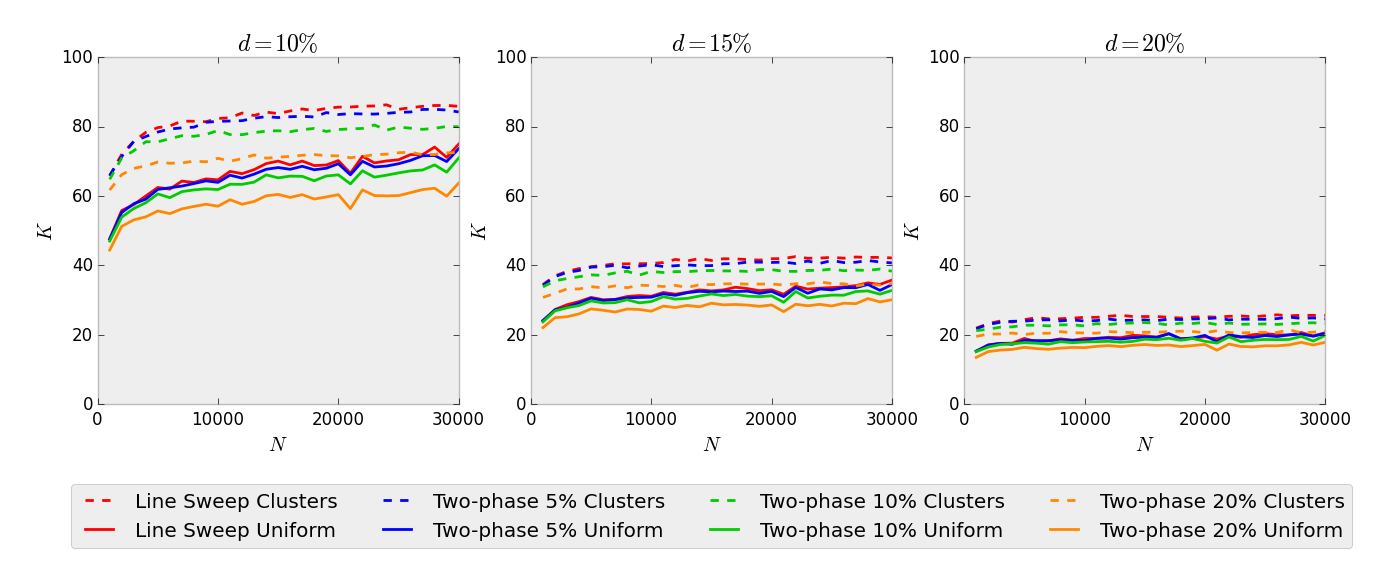
\includegraphics[width=\linewidth]{Pictures/ls_bp_k} 
	\label{fig:ls_bp_k} 
\end{figure}

The graph shows that despite the two-phase algorithms returning lower numbers of $K$, they are not as low as the random sampling. The resulting set does not necessarily cover all the points with disks of radii $d$. Because the first pass transforms the set into disks of radii $d^\prime$, and the second pass only considers their centre point as the measure of cover, then there can be points that are further away from the centroids than $d$, the maximum distance being $d+d^\prime$, as show in Figure \ref{fig:bp_error}.

\begin{figure}[H]
\begin{center}
	
	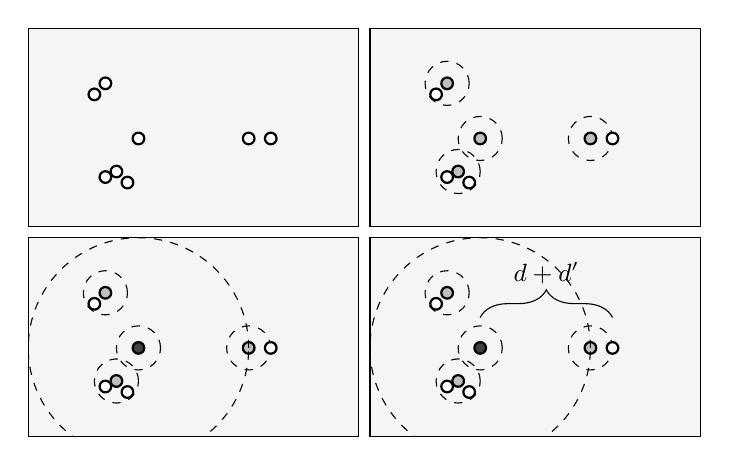
\begin{tikzpicture}[scale=1.4]
	\begin{scope}[]
	\fill[lightgray!15,draw=black] (-1,-0.8) rectangle (2,1);
	\fill[white,draw=black,thick] (0,0) circle (1.5pt);
	\fill[white,draw=black,thick] (1,0) circle (1.5pt);
	\fill[white,draw=black,thick] (1.2,0) circle (1.5pt);
	
	\fill[white,draw=black,thick] (-0.3,0.5) circle (1.5pt);
	\fill[white,draw=black,thick] (-0.4,0.4) circle (1.5pt);
	\fill[white,draw=black,thick] (-0.2,-0.3) circle (1.5pt);
	\fill[white,draw=black,thick] (-0.1,-0.4) circle (1.5pt);
	\fill[white,draw=black,thick] (-0.3,-0.35) circle (1.5pt);
	\end{scope}
	\begin{scope}[shift={(3.1,0)}]
	\fill[lightgray!15,draw=black] (-1,-0.8) rectangle (2,1);
	\fill[lightgray,draw=black,thick] (0,0) circle (1.5pt);
	\fill[lightgray,draw=black,thick] (1,0) circle (1.5pt);
	\fill[lightgray,draw=black,thick] (-0.2,-0.3) circle (1.5pt);
	\fill[lightgray,draw=black,thick] (-0.3,0.5) circle (1.5pt);
	
	\draw[dashed] (0,0) circle (0.2);
	\draw[dashed] (1,0) circle (0.2);
	\draw[dashed] (-0.2,-0.3) circle (0.2);
	\draw[dashed] (-0.3,0.5) circle (0.2);
	
	\fill[white,draw=black,thick] (1.2,0) circle (1.5pt);
	\fill[white,draw=black,thick] (-0.4,0.4) circle (1.5pt);
	\fill[white,draw=black,thick] (-0.1,-0.4) circle (1.5pt);
	\fill[white,draw=black,thick] (-0.3,-0.35) circle (1.5pt);
	\end{scope}
	\begin{scope}[shift={(0,-1.9)}]
	\fill[lightgray!15,draw=black] (-1,-0.8) rectangle (2,1);
	\clip (-1,-0.8) rectangle (2,1);
	
	\fill[darkgray,draw=black,thick] (0,0) circle (1.5pt);
	\fill[lightgray,draw=black,thick] (1,0) circle (1.5pt);
	\fill[lightgray,draw=black,thick] (-0.2,-0.3) circle (1.5pt);
	\fill[lightgray,draw=black,thick] (-0.3,0.5) circle (1.5pt);
	
	
	\draw[dashed] (0,0) circle (1);
	\draw[dashed] (0,0) circle (0.2);
	\draw[dashed] (1,0) circle (0.2);
	\draw[dashed] (-0.2,-0.3) circle (0.2);
	\draw[dashed] (-0.3,0.5) circle (0.2);
	
	\fill[white,draw=black,thick] (1.2,0) circle (1.5pt);
	\fill[white,draw=black,thick] (-0.4,0.4) circle (1.5pt);
	\fill[white,draw=black,thick] (-0.1,-0.4) circle (1.5pt);
	\fill[white,draw=black,thick] (-0.3,-0.35) circle (1.5pt);
	\end{scope}
	
	\begin{scope}[shift={(3.1,-1.9)}]
	\fill[lightgray!15,draw=black] (-1,-0.8) rectangle (2,1);
	\clip (-1,-0.8) rectangle (2,1);
	
	\fill[darkgray,draw=black,thick] (0,0) circle (1.5pt);
	\fill[lightgray,draw=black,thick] (1,0) circle (1.5pt);
	\fill[lightgray,draw=black,thick] (-0.2,-0.3) circle (1.5pt);
	\fill[lightgray,draw=black,thick] (-0.3,0.5) circle (1.5pt);
	
	
	\draw[dashed] (0,0) circle (1);
	\draw[dashed] (0,0) circle (0.2);
	\draw[dashed] (1,0) circle (0.2);
	\draw[dashed] (-0.2,-0.3) circle (0.2);
	\draw[dashed] (-0.3,0.5) circle (0.2);
	
	\fill[white,draw=black,thick] (1.2,0) circle (1.5pt);
	\fill[white,draw=black,thick] (-0.4,0.4) circle (1.5pt);
	\fill[white,draw=black,thick] (-0.1,-0.4) circle (1.5pt);
	\fill[white,draw=black,thick] (-0.3,-0.35) circle (1.5pt);
	
	
	\draw [decorate,decoration={brace,amplitude=10pt,mirror,raise=4pt},yshift=5pt]
	(1.2,0) -- (0,0) node [black,midway,yshift=20] {\small	$d+d'$};
	
	
	\end{scope}
	
	\end{tikzpicture}

\end{center}
\caption{Illustration of the worst case scenario for the error of the biphasic method}
\label{fig:bp_error}
\end{figure}


This result has some effect on the quality, but it is not nearly as noticeable as the results from the random sampling. Figure \ref{fig:bp_sweden} shows the compared output between the original line sweep algorithm, and the different versions of the two-phase algorithm, as well as their intermediate phases.


This final result shows that the two-phase filter, especially with $d^\prime=0.1d$, can yield very approximate results at a fraction of the time, thus making a good candidate to use with inputs larger than the regular Line Sweep method can handle.

\begin{figure}[H]
	\begin{subfigure}[b]{1\linewidth}
		\centering
	\begin{subfigure}[t]{0.29\linewidth}
		\centering
		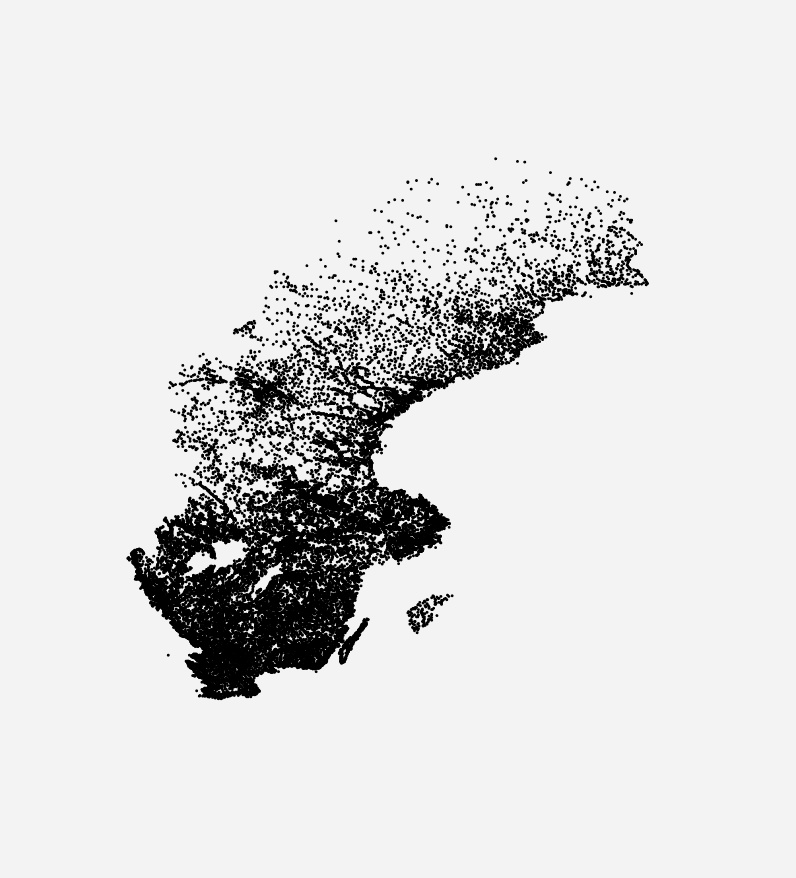
\includegraphics[width=0.9\linewidth]{Pictures/sweden} 
		\caption{} 
		\label{fig:sweden2} 
		\vspace{4ex}
	\end{subfigure}%% 
	\begin{subfigure}[t]{0.29\linewidth}
		\centering
		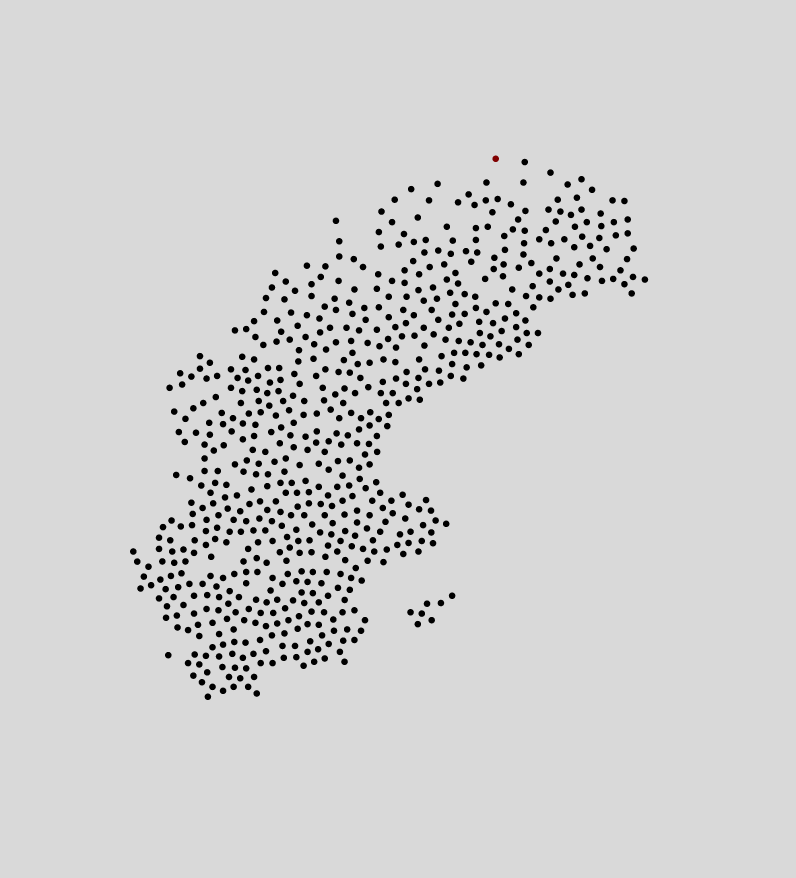
\includegraphics[width=0.9\linewidth]{Pictures/bp5_1_sweden} 
		\caption{} 
		\label{fig:bp5_1_sweden} 
		\vspace{4ex}
	\end{subfigure}
	\begin{subfigure}[t]{0.29\linewidth}
		\centering
		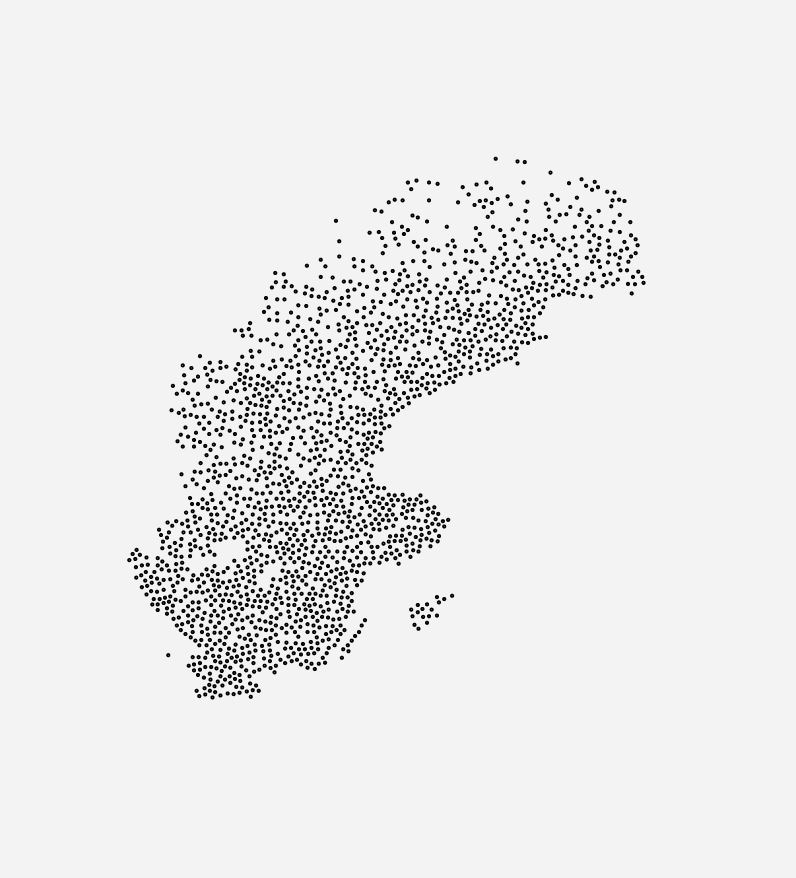
\includegraphics[width=0.9\linewidth]{Pictures/bp10_1_sweden}
		\caption{} 
		\label{fig:bp10_1_sweden} 
		\vspace{4ex}
	\end{subfigure}
\end{subfigure}
\begin{subfigure}[b]{1\linewidth}
	\centering
  \begin{subfigure}[b]{0.29\linewidth}
  	\centering
  	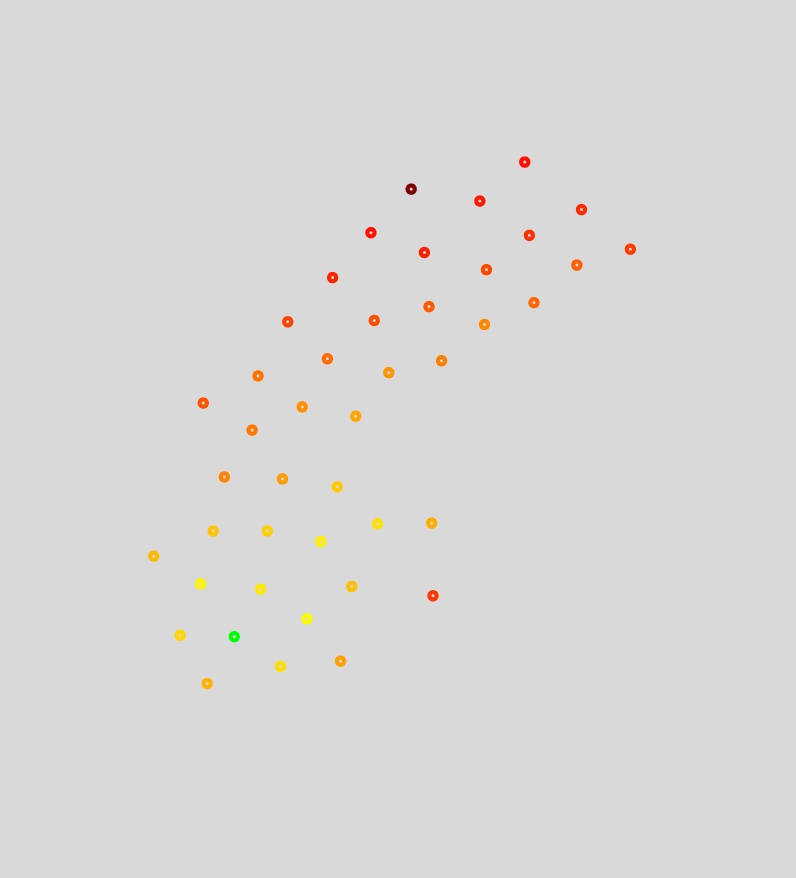
\includegraphics[width=0.9\linewidth]{Pictures/ls_10_sweden} 
  	\caption{} 
  	\label{fig:ls_10_sweden2} 
  	\vspace{4ex}
  \end{subfigure}%% 
  \begin{subfigure}[b]{0.29\linewidth}
  	\centering
  	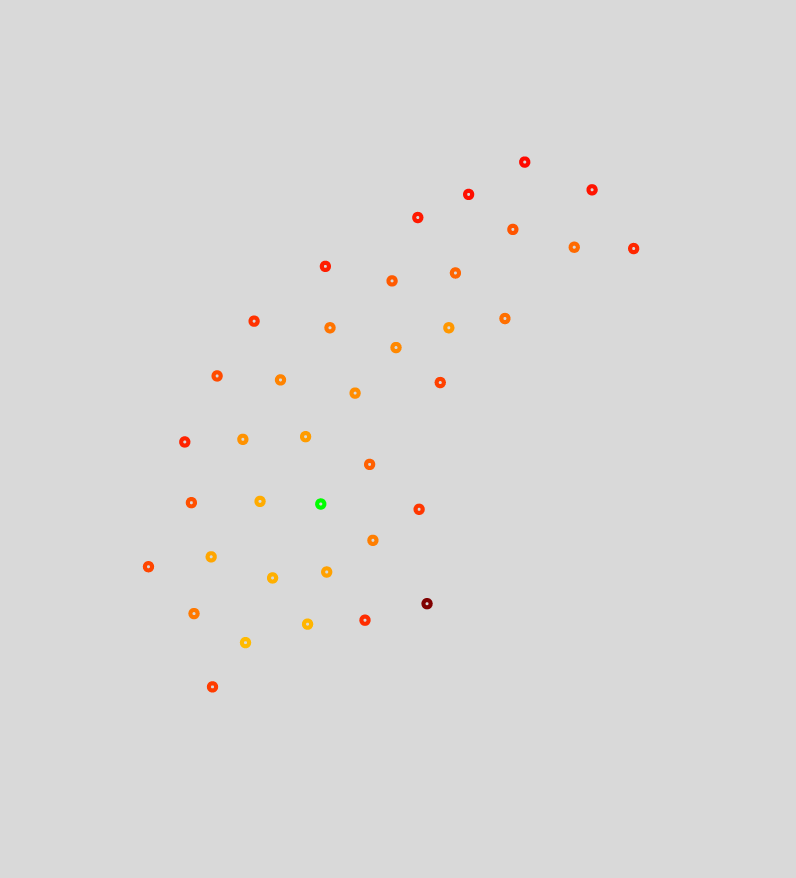
\includegraphics[width=0.9\linewidth]{Pictures/bp5_2_sweden} 
  	\caption{} 
  	\label{fig:bp5_2_sweden} 
  	\vspace{4ex}
  \end{subfigure}
  \begin{subfigure}[b]{0.29\linewidth}
  	\centering
  	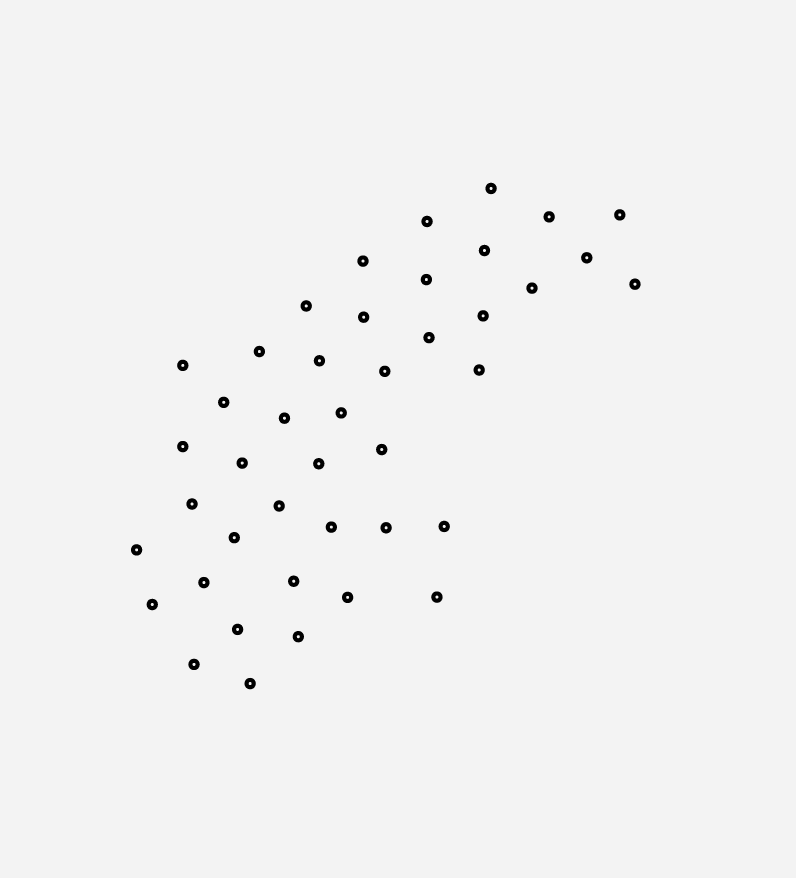
\includegraphics[width=0.9\linewidth]{Pictures/bp10_2_sweden} 
  	\caption{} 
  	\label{fig:bp10_2_sweden} 
  	\vspace{4ex}
  \end{subfigure}
\end{subfigure}
  \caption{Biphasic Filter result comparison.}
  \centering \small
  \parbox{0.5\linewidth}{(A) Original Set (B) Intermediate Set for Biphasic Filter with $d'=0.05d$ (C) Intermediate Set for Biphasic Filter with $d'=0.1d$ (D) Final Set for one pass (E) Final Set for Biphasic Filter with $d'=0.05d$ (F) Final Set for Biphasic Filter with $d'=0.1d$ }
  \label{fig:bp_sweden} 
\end{figure}



\section{Region Panning and Zooming}
\begin{change}
One of the requirements established for the final algorithm it that it should be able to handle a translation motion in the region and starting point set. This means that in case the new region intersects the previous one, it is important for the user that the points already in display are kept selected, so that each move does not cause the user to . As such, any selected centroids inside the intersection of the two regions, and all the points covered by them, should be kept unchanged, even if it means losing the guaranteed approximation to the optimal value. Each of the approaches described earlier can be modified to ensure that this property is met. 

To handle the panning case, each instance of the program receives the centroids chosen in the previous region. To ensure that the points are still selected is a matter of artificially increasing their number of neighbours by $N$, then compute the problem regularly.  Since the number of points from the old region is bound above by at most 128, the new number of points is relatively insignificant for instances of 10000 points and more, and the algorithms show no significant difference in performance. Since the covering distance does not change, the old centroids are not close enough together to cover each other, otherwise they would have done so in the old region. This solves the panning issue without needing to add much complexity to the algorithms. In the case of multiple phase filters, the weight of the selected points must be artificially increased in all the phases, to ensure they are kept selected.

\begin{figure}[!h]
	\centering	
	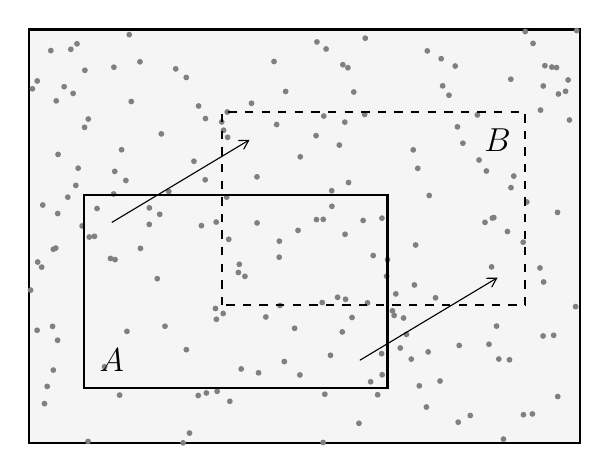
\begin{tikzpicture}[scale=0.35]
	\fill[lightgray!15,draw=black,thick] (0,0) rectangle (20,15);
	
	\fill[gray] (7.189873,12.007256) circle (3pt);
	\fill[gray] (1.032745,3.725546) circle (3pt);
	\fill[gray] (5.703827,13.261152) circle (3pt);
	\fill[gray] (17.936429,1.025270) circle (3pt);
	\fill[gray] (13.690591,3.939102) circle (3pt);
	\fill[gray] (11.193998,5.283551) circle (3pt);
	\fill[gray] (4.798022,11.213652) circle (3pt);
	\fill[gray] (18.715176,13.688003) circle (3pt);
	\fill[gray] (10.692704,11.860352) circle (3pt);
	\fill[gray] (7.056115,11.346718) circle (3pt);
	\fill[gray] (0.966585,7.071031) circle (3pt);
	\fill[gray] (13.937926,10.633255) circle (3pt);
	\fill[gray] (7.593829,6.185742) circle (3pt);
	\fill[gray] (3.705931,12.388078) circle (3pt);
	\fill[gray] (10.775614,14.295963) circle (3pt);
	\fill[gray] (18.057741,8.744112) circle (3pt);
	\fill[gray] (8.068603,12.323568) circle (3pt);
	\fill[gray] (18.650144,3.881699) circle (3pt);
	\fill[gray] (12.484510,6.800151) circle (3pt);
	\fill[gray] (13.183608,4.794407) circle (3pt);
	\fill[gray] (12.174938,11.920051) circle (3pt);
	\fill[gray] (1.736886,14.482144) circle (3pt);
	\fill[gray] (3.355545,10.638588) circle (3pt);
	\fill[gray] (0.295411,13.134745) circle (3pt);
	\fill[gray] (17.430353,3.016958) circle (3pt);
	\fill[gray] (19.869400,14.962442) circle (3pt);
	\fill[gray] (10.729442,1.767601) circle (3pt);
	\fill[gray] (0.984080,12.412868) circle (3pt);
	\fill[gray] (0.656211,2.050832) circle (3pt);
	\fill[gray] (6.149162,12.226380) circle (3pt);
	\fill[gray] (10.443128,14.550410) circle (3pt);
	\fill[gray] (18.655995,12.951857) circle (3pt);
	\fill[gray] (11.590530,9.448236) circle (3pt);
	\fill[gray] (7.243261,7.388230) circle (3pt);
	\fill[gray] (18.260829,1.052094) circle (3pt);
	\fill[gray] (9.825389,2.467039) circle (3pt);
	\fill[gray] (1.270561,12.927529) circle (3pt);
	\fill[gray] (2.183670,7.471334) circle (3pt);
	\fill[gray] (9.101712,4.988481) circle (3pt);
	\fill[gray] (2.138719,0.055549) circle (3pt);
	\fill[gray] (6.399133,11.770019) circle (3pt);
	\fill[gray] (16.541260,8.003890) circle (3pt);
	\fill[gray] (11.256169,10.807615) circle (3pt);
	\fill[gray] (17.926257,7.283852) circle (3pt);
	\fill[gray] (2.739774,2.765903) circle (3pt);
	\fill[gray] (18.966992,13.637273) circle (3pt);
	\fill[gray] (10.668147,0.016967) circle (3pt);
	\fill[gray] (0.310205,6.564354) circle (3pt);
	\fill[gray] (12.811328,2.473994) circle (3pt);
	\fill[gray] (11.566809,13.614052) circle (3pt);
	\fill[gray] (3.283881,1.735554) circle (3pt);
	\fill[gray] (14.101612,9.963662) circle (3pt);
	\fill[gray] (4.039885,7.059605) circle (3pt);
	\fill[gray] (16.591664,9.866772) circle (3pt);
	\fill[gray] (14.517395,8.977751) circle (3pt);
	\fill[gray] (10.426222,8.104159) circle (3pt);
	\fill[gray] (3.549166,4.048136) circle (3pt);
	\fill[gray] (17.483642,9.263434) circle (3pt);
	\fill[gray] (16.325371,10.266466) circle (3pt);
	\fill[gray] (10.979845,9.152594) circle (3pt);
	\fill[gray] (5.981012,10.220922) circle (3pt);
	\fill[gray] (13.465983,3.443126) circle (3pt);
	\fill[gray] (6.251647,7.884290) circle (3pt);
	\fill[gray] (4.363000,8.528955) circle (3pt);
	\fill[gray] (11.463047,7.570383) circle (3pt);
	\fill[gray] (6.761937,4.878485) circle (3pt);
	\fill[gray] (12.392466,2.219189) circle (3pt);
	\fill[gray] (15.739529,10.876258) circle (3pt);
	\fill[gray] (11.362909,4.028322) circle (3pt);
	\fill[gray] (1.403271,8.917787) circle (3pt);
	\fill[gray] (1.694522,9.344248) circle (3pt);
	\fill[gray] (4.738868,8.295962) circle (3pt);
	\fill[gray] (6.389808,9.547780) circle (3pt);
	\fill[gray] (8.886094,13.840983) circle (3pt);
	\fill[gray] (7.040599,4.696280) circle (3pt);
	\fill[gray] (14.952140,13.942108) circle (3pt);
	\fill[gray] (17.211416,0.139226) circle (3pt);
	\fill[gray] (10.670952,8.112072) circle (3pt);
	\fill[gray] (9.839079,10.382850) circle (3pt);
	\fill[gray] (16.809571,8.160259) circle (3pt);
	\fill[gray] (17.478862,13.197850) circle (3pt);
	\fill[gray] (16.008395,0.995887) circle (3pt);
	\fill[gray] (6.135184,1.721209) circle (3pt);
	\fill[gray] (7.202958,11.088303) circle (3pt);
	\fill[gray] (15.604905,3.537251) circle (3pt);
	\fill[gray] (4.649788,5.960632) circle (3pt);
	\fill[gray] (12.646831,1.748152) circle (3pt);
	\fill[gray] (5.704931,3.385258) circle (3pt);
	\fill[gray] (13.244499,4.627266) circle (3pt);
	\fill[gray] (13.866541,3.042211) circle (3pt);
	\fill[gray] (4.020821,13.829378) circle (3pt);
	\fill[gray] (14.478915,3.303659) circle (3pt);
	\fill[gray] (12.119582,8.071522) circle (3pt);
	\fill[gray] (0.052974,5.544991) circle (3pt);
	\fill[gray] (14.157844,2.072198) circle (3pt);
	\fill[gray] (19.829076,4.945795) circle (3pt);
	\fill[gray] (19.464476,12.758033) circle (3pt);
	\fill[gray] (14.448449,14.224297) circle (3pt);
	\fill[gray] (8.325068,2.544047) circle (3pt);
	\fill[gray] (4.359520,7.930448) circle (3pt);
	\fill[gray] (3.633524,14.815104) circle (3pt);
	\fill[gray] (17.042602,3.044707) circle (3pt);
	\fill[gray] (11.717216,4.551330) circle (3pt);
	\fill[gray] (0.494682,8.633230) circle (3pt);
	\fill[gray] (13.979299,5.732816) circle (3pt);
	\fill[gray] (18.535276,6.350147) circle (3pt);
	\fill[gray] (8.267637,9.654893) circle (3pt);
	\fill[gray] (0.880287,7.026485) circle (3pt);
	\fill[gray] (7.695881,2.684383) circle (3pt);
	\fill[gray] (2.465090,8.505883) circle (3pt);
	\fill[gray] (14.415714,1.302376) circle (3pt);
	\fill[gray] (15.569702,0.753946) circle (3pt);
	\fill[gray] (18.285254,14.497479) circle (3pt);
	\fill[gray] (0.455887,6.378918) circle (3pt);
	\fill[gray] (12.197111,14.685628) circle (3pt);
	\fill[gray] (6.795592,4.486260) circle (3pt);
	\fill[gray] (16.686419,3.579784) circle (3pt);
	\fill[gray] (3.510219,9.522966) circle (3pt);
	\fill[gray] (6.822231,1.872439) circle (3pt);
	\fill[gray] (1.037286,8.323394) circle (3pt);
	\fill[gray] (18.556981,12.076557) circle (3pt);
	\fill[gray] (3.117391,6.651586) circle (3pt);
	\fill[gray] (13.304852,5.408005) circle (3pt);
	\fill[gray] (2.023153,13.521868) circle (3pt);
	\fill[gray] (2.147448,11.752045) circle (3pt);
	\fill[gray] (9.632847,4.159554) circle (3pt);
	\fill[gray] (2.012655,11.451130) circle (3pt);
	\fill[gray] (19.605825,11.716914) circle (3pt);
	\fill[gray] (10.634260,5.094222) circle (3pt);
	\fill[gray] (4.929862,4.234030) circle (3pt);
	\fill[gray] (11.779346,12.733778) circle (3pt);
	\fill[gray] (17.355771,7.671409) circle (3pt);
	\fill[gray] (16.264088,11.902180) circle (3pt);
	\fill[gray] (0.851292,4.229110) circle (3pt);
	\fill[gray] (14.911070,2.246137) circle (3pt);
	\fill[gray] (12.790055,3.240956) circle (3pt);
	\fill[gray] (3.106337,9.853823) circle (3pt);
	\fill[gray] (15.004812,12.957114) circle (3pt);
	\fill[gray] (11.455350,11.640517) circle (3pt);
	\fill[gray] (16.862233,8.176758) circle (3pt);
	\fill[gray] (7.283005,1.511903) circle (3pt);
	\fill[gray] (14.023672,7.183187) circle (3pt);
	\fill[gray] (16.959859,4.239292) circle (3pt);
	\fill[gray] (9.080443,7.321678) circle (3pt);
	\fill[gray] (0.787920,14.235724) circle (3pt);
	\fill[gray] (9.757357,7.711644) circle (3pt);
	\fill[gray] (12.801919,8.156807) circle (3pt);
	\fill[gray] (19.173654,8.365171) circle (3pt);
	\fill[gray] (14.746939,5.266785) circle (3pt);
	\fill[gray] (15.460890,13.675672) circle (3pt);
	\fill[gray] (0.558498,1.426722) circle (3pt);
	\fill[gray] (5.319326,13.573341) circle (3pt);
	\fill[gray] (1.596066,12.682471) circle (3pt);
	\fill[gray] (10.411521,11.148780) circle (3pt);
	\fill[gray] (15.234786,12.617005) circle (3pt);
	\fill[gray] (0.878152,2.643967) circle (3pt);
	\fill[gray] (2.952409,6.694919) circle (3pt);
	\fill[gray] (9.074063,6.740000) circle (3pt);
	\fill[gray] (15.540580,11.468732) circle (3pt);
	\fill[gray] (18.001669,14.926523) circle (3pt);
	\fill[gray] (19.206391,12.660252) circle (3pt);
	\fill[gray] (13.006573,6.651786) circle (3pt);
	\fill[gray] (1.513548,14.283169) circle (3pt);
	\fill[gray] (7.830906,6.044319) circle (3pt);
	\fill[gray] (18.668757,5.840355) circle (3pt);
	\fill[gray] (12.281253,5.082468) circle (3pt);
	\fill[gray] (16.780682,6.387540) circle (3pt);
	\fill[gray] (11.968683,0.711781) circle (3pt);
	\fill[gray] (6.788235,8.014438) circle (3pt);
	\fill[gray] (0.289549,4.087150) circle (3pt);
	\fill[gray] (12.971851,6.048889) circle (3pt);
	\fill[gray] (3.067813,9.033496) circle (3pt);
	\fill[gray] (5.068369,9.124380) circle (3pt);
	\fill[gray] (5.587748,0.003656) circle (3pt);
	\fill[gray] (13.586570,4.533691) circle (3pt);
	\fill[gray] (6.431809,1.813709) circle (3pt);
	\fill[gray] (0.119261,12.849029) circle (3pt);
	\fill[gray] (11.383318,13.725656) circle (3pt);
	\fill[gray] (3.075973,13.633286) circle (3pt);
	\fill[gray] (8.271872,7.982950) circle (3pt);
	\fill[gray] (9.259674,2.953089) circle (3pt);
	\fill[gray] (9.308203,12.753614) circle (3pt);
	\fill[gray] (1.923948,7.874574) circle (3pt);
	\fill[gray] (10.934866,3.180220) circle (3pt);
	\fill[gray] (19.138825,13.620963) circle (3pt);
	\fill[gray] (7.627648,6.481897) circle (3pt);
	\fill[gray] (19.180860,1.683719) circle (3pt);
	\fill[gray] (8.589508,4.571152) circle (3pt);
	\fill[gray] (7.168202,8.919764) circle (3pt);
	\fill[gray] (17.585780,9.683140) circle (3pt);
	\fill[gray] (10.985187,8.586106) circle (3pt);
	\fill[gray] (8.981215,11.553663) circle (3pt);
	\fill[gray] (11.481412,5.212075) circle (3pt);
	\fill[gray] (19.557651,13.170481) circle (3pt);
	\fill[gray] (1.779307,9.969640) circle (3pt);
	\fill[gray] (19.033129,3.905117) circle (3pt);
	\fill[gray] (1.050651,10.469207) circle (3pt);
	\fill[gray] (2.370389,7.496352) circle (3pt);
	\fill[gray] (6.988479,11.647790) circle (3pt);
	\fill[gray] (5.818615,0.357924) circle (3pt);
	
	\draw[black,thick] (2,2) rectangle (13,9);
	\draw[black,thick,dashed] (7,5) rectangle (18,12);
	\draw[->,>=angle 60,black] (3,8) --(8,11);
	\draw[->,>=angle 60,black] (12,3) -- (17,6);
	\node at (3,3) {\large $A$};
	\node at (17,11) {\large $B$};
	
	\end{tikzpicture}
	\caption[Example of a panning motion]{Example of a panning motion from region $A$ to region $B$. Centroids contained in $A \cap B$ calculated in region $A$ must be kept when calculating region $B$.}
	\label{fig:panning}
\end{figure}

In the case of zooming, the scale changes, and so does the minimum distance. The points selected previously are relatively more close together in the new window, and they shift towards the centre of the region. One of the solutions is to simply discard the previous selected points, since they do not have the same representation properties they did in the previous region. Another solution is to do the same process as for the panning. By artificially inflating the weight of the established points, they is given priority over the new window's points. Since the points are now close together, they may cover each other, and some inevitably cease to be selected.

\begin{figure}[!h]
	\centering
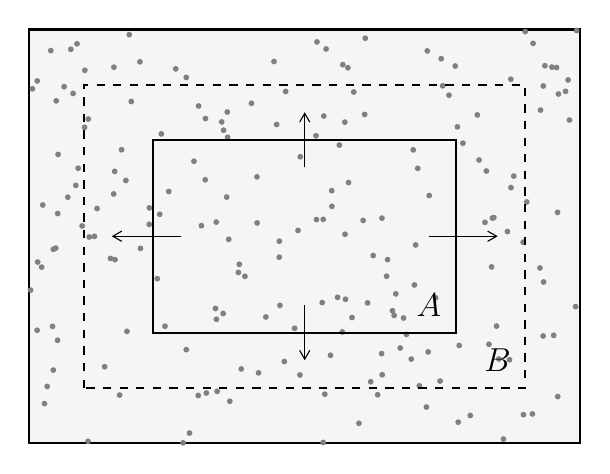
\begin{tikzpicture}[scale=0.35]
\fill[lightgray!15,draw=black,thick] (0,0) rectangle (20,15);

\fill[gray] (7.189873,12.007256) circle (3pt);
\fill[gray] (1.032745,3.725546) circle (3pt);
\fill[gray] (5.703827,13.261152) circle (3pt);
\fill[gray] (17.936429,1.025270) circle (3pt);
\fill[gray] (13.690591,3.939102) circle (3pt);
\fill[gray] (11.193998,5.283551) circle (3pt);
\fill[gray] (4.798022,11.213652) circle (3pt);
\fill[gray] (18.715176,13.688003) circle (3pt);
\fill[gray] (10.692704,11.860352) circle (3pt);
\fill[gray] (7.056115,11.346718) circle (3pt);
\fill[gray] (0.966585,7.071031) circle (3pt);
\fill[gray] (13.937926,10.633255) circle (3pt);
\fill[gray] (7.593829,6.185742) circle (3pt);
\fill[gray] (3.705931,12.388078) circle (3pt);
\fill[gray] (10.775614,14.295963) circle (3pt);
\fill[gray] (18.057741,8.744112) circle (3pt);
\fill[gray] (8.068603,12.323568) circle (3pt);
\fill[gray] (18.650144,3.881699) circle (3pt);
\fill[gray] (12.484510,6.800151) circle (3pt);
\fill[gray] (13.183608,4.794407) circle (3pt);
\fill[gray] (12.174938,11.920051) circle (3pt);
\fill[gray] (1.736886,14.482144) circle (3pt);
\fill[gray] (3.355545,10.638588) circle (3pt);
\fill[gray] (0.295411,13.134745) circle (3pt);
\fill[gray] (17.430353,3.016958) circle (3pt);
\fill[gray] (19.869400,14.962442) circle (3pt);
\fill[gray] (10.729442,1.767601) circle (3pt);
\fill[gray] (0.984080,12.412868) circle (3pt);
\fill[gray] (0.656211,2.050832) circle (3pt);
\fill[gray] (6.149162,12.226380) circle (3pt);
\fill[gray] (10.443128,14.550410) circle (3pt);
\fill[gray] (18.655995,12.951857) circle (3pt);
\fill[gray] (11.590530,9.448236) circle (3pt);
\fill[gray] (7.243261,7.388230) circle (3pt);
\fill[gray] (18.260829,1.052094) circle (3pt);
\fill[gray] (9.825389,2.467039) circle (3pt);
\fill[gray] (1.270561,12.927529) circle (3pt);
\fill[gray] (2.183670,7.471334) circle (3pt);
\fill[gray] (9.101712,4.988481) circle (3pt);
\fill[gray] (2.138719,0.055549) circle (3pt);
\fill[gray] (6.399133,11.770019) circle (3pt);
\fill[gray] (16.541260,8.003890) circle (3pt);
\fill[gray] (11.256169,10.807615) circle (3pt);
\fill[gray] (17.926257,7.283852) circle (3pt);
\fill[gray] (2.739774,2.765903) circle (3pt);
\fill[gray] (18.966992,13.637273) circle (3pt);
\fill[gray] (10.668147,0.016967) circle (3pt);
\fill[gray] (0.310205,6.564354) circle (3pt);
\fill[gray] (12.811328,2.473994) circle (3pt);
\fill[gray] (11.566809,13.614052) circle (3pt);
\fill[gray] (3.283881,1.735554) circle (3pt);
\fill[gray] (14.101612,9.963662) circle (3pt);
\fill[gray] (4.039885,7.059605) circle (3pt);
\fill[gray] (16.591664,9.866772) circle (3pt);
\fill[gray] (14.517395,8.977751) circle (3pt);
\fill[gray] (10.426222,8.104159) circle (3pt);
\fill[gray] (3.549166,4.048136) circle (3pt);
\fill[gray] (17.483642,9.263434) circle (3pt);
\fill[gray] (16.325371,10.266466) circle (3pt);
\fill[gray] (10.979845,9.152594) circle (3pt);
\fill[gray] (5.981012,10.220922) circle (3pt);
\fill[gray] (13.465983,3.443126) circle (3pt);
\fill[gray] (6.251647,7.884290) circle (3pt);
\fill[gray] (4.363000,8.528955) circle (3pt);
\fill[gray] (11.463047,7.570383) circle (3pt);
\fill[gray] (6.761937,4.878485) circle (3pt);
\fill[gray] (12.392466,2.219189) circle (3pt);
\fill[gray] (15.739529,10.876258) circle (3pt);
\fill[gray] (11.362909,4.028322) circle (3pt);
\fill[gray] (1.403271,8.917787) circle (3pt);
\fill[gray] (1.694522,9.344248) circle (3pt);
\fill[gray] (4.738868,8.295962) circle (3pt);
\fill[gray] (6.389808,9.547780) circle (3pt);
\fill[gray] (8.886094,13.840983) circle (3pt);
\fill[gray] (7.040599,4.696280) circle (3pt);
\fill[gray] (14.952140,13.942108) circle (3pt);
\fill[gray] (17.211416,0.139226) circle (3pt);
\fill[gray] (10.670952,8.112072) circle (3pt);
\fill[gray] (9.839079,10.382850) circle (3pt);
\fill[gray] (16.809571,8.160259) circle (3pt);
\fill[gray] (17.478862,13.197850) circle (3pt);
\fill[gray] (16.008395,0.995887) circle (3pt);
\fill[gray] (6.135184,1.721209) circle (3pt);
\fill[gray] (7.202958,11.088303) circle (3pt);
\fill[gray] (15.604905,3.537251) circle (3pt);
\fill[gray] (4.649788,5.960632) circle (3pt);
\fill[gray] (12.646831,1.748152) circle (3pt);
\fill[gray] (5.704931,3.385258) circle (3pt);
\fill[gray] (13.244499,4.627266) circle (3pt);
\fill[gray] (13.866541,3.042211) circle (3pt);
\fill[gray] (4.020821,13.829378) circle (3pt);
\fill[gray] (14.478915,3.303659) circle (3pt);
\fill[gray] (12.119582,8.071522) circle (3pt);
\fill[gray] (0.052974,5.544991) circle (3pt);
\fill[gray] (14.157844,2.072198) circle (3pt);
\fill[gray] (19.829076,4.945795) circle (3pt);
\fill[gray] (19.464476,12.758033) circle (3pt);
\fill[gray] (14.448449,14.224297) circle (3pt);
\fill[gray] (8.325068,2.544047) circle (3pt);
\fill[gray] (4.359520,7.930448) circle (3pt);
\fill[gray] (3.633524,14.815104) circle (3pt);
\fill[gray] (17.042602,3.044707) circle (3pt);
\fill[gray] (11.717216,4.551330) circle (3pt);
\fill[gray] (0.494682,8.633230) circle (3pt);
\fill[gray] (13.979299,5.732816) circle (3pt);
\fill[gray] (18.535276,6.350147) circle (3pt);
\fill[gray] (8.267637,9.654893) circle (3pt);
\fill[gray] (0.880287,7.026485) circle (3pt);
\fill[gray] (7.695881,2.684383) circle (3pt);
\fill[gray] (2.465090,8.505883) circle (3pt);
\fill[gray] (14.415714,1.302376) circle (3pt);
\fill[gray] (15.569702,0.753946) circle (3pt);
\fill[gray] (18.285254,14.497479) circle (3pt);
\fill[gray] (0.455887,6.378918) circle (3pt);
\fill[gray] (12.197111,14.685628) circle (3pt);
\fill[gray] (6.795592,4.486260) circle (3pt);
\fill[gray] (16.686419,3.579784) circle (3pt);
\fill[gray] (3.510219,9.522966) circle (3pt);
\fill[gray] (6.822231,1.872439) circle (3pt);
\fill[gray] (1.037286,8.323394) circle (3pt);
\fill[gray] (18.556981,12.076557) circle (3pt);
\fill[gray] (3.117391,6.651586) circle (3pt);
\fill[gray] (13.304852,5.408005) circle (3pt);
\fill[gray] (2.023153,13.521868) circle (3pt);
\fill[gray] (2.147448,11.752045) circle (3pt);
\fill[gray] (9.632847,4.159554) circle (3pt);
\fill[gray] (2.012655,11.451130) circle (3pt);
\fill[gray] (19.605825,11.716914) circle (3pt);
\fill[gray] (10.634260,5.094222) circle (3pt);
\fill[gray] (4.929862,4.234030) circle (3pt);
\fill[gray] (11.779346,12.733778) circle (3pt);
\fill[gray] (17.355771,7.671409) circle (3pt);
\fill[gray] (16.264088,11.902180) circle (3pt);
\fill[gray] (0.851292,4.229110) circle (3pt);
\fill[gray] (14.911070,2.246137) circle (3pt);
\fill[gray] (12.790055,3.240956) circle (3pt);
\fill[gray] (3.106337,9.853823) circle (3pt);
\fill[gray] (15.004812,12.957114) circle (3pt);
\fill[gray] (11.455350,11.640517) circle (3pt);
\fill[gray] (16.862233,8.176758) circle (3pt);
\fill[gray] (7.283005,1.511903) circle (3pt);
\fill[gray] (14.023672,7.183187) circle (3pt);
\fill[gray] (16.959859,4.239292) circle (3pt);
\fill[gray] (9.080443,7.321678) circle (3pt);
\fill[gray] (0.787920,14.235724) circle (3pt);
\fill[gray] (9.757357,7.711644) circle (3pt);
\fill[gray] (12.801919,8.156807) circle (3pt);
\fill[gray] (19.173654,8.365171) circle (3pt);
\fill[gray] (14.746939,5.266785) circle (3pt);
\fill[gray] (15.460890,13.675672) circle (3pt);
\fill[gray] (0.558498,1.426722) circle (3pt);
\fill[gray] (5.319326,13.573341) circle (3pt);
\fill[gray] (1.596066,12.682471) circle (3pt);
\fill[gray] (10.411521,11.148780) circle (3pt);
\fill[gray] (15.234786,12.617005) circle (3pt);
\fill[gray] (0.878152,2.643967) circle (3pt);
\fill[gray] (2.952409,6.694919) circle (3pt);
\fill[gray] (9.074063,6.740000) circle (3pt);
\fill[gray] (15.540580,11.468732) circle (3pt);
\fill[gray] (18.001669,14.926523) circle (3pt);
\fill[gray] (19.206391,12.660252) circle (3pt);
\fill[gray] (13.006573,6.651786) circle (3pt);
\fill[gray] (1.513548,14.283169) circle (3pt);
\fill[gray] (7.830906,6.044319) circle (3pt);
\fill[gray] (18.668757,5.840355) circle (3pt);
\fill[gray] (12.281253,5.082468) circle (3pt);
\fill[gray] (16.780682,6.387540) circle (3pt);
\fill[gray] (11.968683,0.711781) circle (3pt);
\fill[gray] (6.788235,8.014438) circle (3pt);
\fill[gray] (0.289549,4.087150) circle (3pt);
\fill[gray] (12.971851,6.048889) circle (3pt);
\fill[gray] (3.067813,9.033496) circle (3pt);
\fill[gray] (5.068369,9.124380) circle (3pt);
\fill[gray] (5.587748,0.003656) circle (3pt);
\fill[gray] (13.586570,4.533691) circle (3pt);
\fill[gray] (6.431809,1.813709) circle (3pt);
\fill[gray] (0.119261,12.849029) circle (3pt);
\fill[gray] (11.383318,13.725656) circle (3pt);
\fill[gray] (3.075973,13.633286) circle (3pt);
\fill[gray] (8.271872,7.982950) circle (3pt);
\fill[gray] (9.259674,2.953089) circle (3pt);
\fill[gray] (9.308203,12.753614) circle (3pt);
\fill[gray] (1.923948,7.874574) circle (3pt);
\fill[gray] (10.934866,3.180220) circle (3pt);
\fill[gray] (19.138825,13.620963) circle (3pt);
\fill[gray] (7.627648,6.481897) circle (3pt);
\fill[gray] (19.180860,1.683719) circle (3pt);
\fill[gray] (8.589508,4.571152) circle (3pt);
\fill[gray] (7.168202,8.919764) circle (3pt);
\fill[gray] (17.585780,9.683140) circle (3pt);
\fill[gray] (10.985187,8.586106) circle (3pt);
\fill[gray] (8.981215,11.553663) circle (3pt);
\fill[gray] (11.481412,5.212075) circle (3pt);
\fill[gray] (19.557651,13.170481) circle (3pt);
\fill[gray] (1.779307,9.969640) circle (3pt);
\fill[gray] (19.033129,3.905117) circle (3pt);
\fill[gray] (1.050651,10.469207) circle (3pt);
\fill[gray] (2.370389,7.496352) circle (3pt);
\fill[gray] (6.988479,11.647790) circle (3pt);
\fill[gray] (5.818615,0.357924) circle (3pt);

\draw[black,thick] (4.5,4) rectangle (15.5,11);
\draw[black,thick,dashed] (2,2) rectangle (18,13);
\draw[->,>=angle 60,black] (10,10) --(10,12);
\draw[->,>=angle 60,black] (10,5) --(10,3);
\draw[->,>=angle 60,black] (14.5,7.5) -- (17,7.5);
\draw[->,>=angle 60,black] (5.5,7.5) -- (3,7.5);
\node at (14.5,5) {\large $A$};
\node at (17,3) {\large $B$};

\end{tikzpicture}
\caption[Example of a zooming motion]{Example of a zooming motion from region $A$ to region $B$. Centroids contained in $A \cap B$ calculated in region $A$ should have selection priority when calculating region $B$.}
\label{fig:zooming}
\end{figure}

\section{Discussion}
The approximation algorithms in this chapter meet the efficiency requirements established for the web application, and are also able to handle panning and zooming motions without any complexity. In the case the test inputs prove to still be too large to be handled by the approximation algorithms, a good alternative is found in the Two-phase filtering approach.

A solution for even larger set of points may require more filter phases, but for the inputs given, no such solution was needed. Furthermore, since the two-phase filtering approaches show similar times to the random sampling approaches, while showing fewer critical shortcomings, there should be no advantage in using random sampling.

\end{change} 
%\chapter{Future Work}
\label{chap:future}
\lhead{Chapter \ref{chap:future}. \emph{\nameref{chap:future}}}
\section{Integration in a Visualisation Framework}
\paragraph{}
The final objective of this study is to integrate an algorithm in a web application that can display the most representative set. There is, however, a time constraint to do this. The feedback time on the application needs to be as small as possible while still delivering an acceptable set of points, in order to not lose engagement from the user.
\paragraph{}
The application will display a rectangular window, showing a cut of geographical region containing a set of points. The algorithm chosen will need to be able to choose a representative set of points within the cut quickly, as well as be able to recalculate a new set points for a new cut, resulting from panning or zooming the display window over the region.
\paragraph{}
The algorithm serve as the middleware responsible for filtering the response of a GIS server to a Web Map Service, or WMS request. WMS lists the geographic coordinates of the points to be represented in an image by the coordinates mapped into orthogonally organised pixels on an image displaying the cut of the region requested by the application.
The candidate algorithms will be tested and benchmarked using data from the Open Street Map project. The project features large quantities of open source geographic data, as well as a versatile API for fetching data in the WMS standard.
\section{Heuristic Approaches}
\paragraph{}
Optimal solution algorithms, and their slow time performance, makes them a poor choice for real-time applications. As such, heuristic algorithms that provide good but not optimal solution in faster time are more likely the most appropriate approach.
Since a lot of complex structures have already been explored and implemented in the implicit enumeration approaches, a lot of the concepts and methods can be repurposed and reused when experimenting and researching heuristic approaches. 
\change{
	\paragraph{}
	For instance, since the two interactions with any calculated solution will be panning and zooming, some new solutions may share some points. If that is the case, calculating a solution after a small pan or zoom may reuse the previously calculated region as a starting point, only adding the new points, and removing the previously calculated ones.
	\paragraph{}
	An extension to this method may include calculating a larger area than the queried one, so that a small pan and/or zoom include already calculating data. After the window moves, the new adjacent regions can be calculated. This way, the user should never see the window without processed data, and the program will only calculate areas outside the vision range of the window.
}
	\section {Approximation Algorithms}
\change{
	\paragraph{}
	Approximation algorithms are used to used in optimisation as a means to achieve a valid solution within a guaranteed minimum factor of quality to the optimal solution. Ideally, the approximation is optimal up to a constant factor, the smaller the better. Approximation algorithms have been found and described by \citet{approx}, that give an approximation with a factor of $3.16$ to the optimal solution of \emph{p-center} problem.
}
%
%\section{Uniformity}
%\paragraph{}
%Another measure of quality for a solution is its \emph{uniformity}. Uniformity is defined mathematically in a set of points as the distance between the closest pair of points. The most representative subset $U$ of a larger set $N$ relative to its uniformity will be the subset of $N$ that has the highest value for the distance of its closest pair. Like coverage, the concept of uniformity is frequent in the field of optimisation. Maximising uniformity can be formally defined as:
%
%\begin{equation}
%\max_{U \in N}{\min_{\substack{u_i,u_j \in U \\ u_i \neq u_j}}{\lVert u_i-u_j \rVert}}
%\end{equation}
%
%\noindent
%Where $N$ is the initial set of points in $\mathbb{R}^2$, $U$ is the most uniform subset in $N$, and $\lVert \cdot \rVert$ is the Euclidean distance between two points. The maximum uniformity is the most representative set. 
%\cleardoublepage
\chapter{Conclusion}
\label{chap:conc}
\lhead{Chapter \ref{chap:conc}. \emph{\nameref{chap:conc}}}
\vspace{-15pt}
In this thesis, we designed algorithms to select representative subsets from large quantities of geographic points. The algorithm must be able to handle panning and zooming motions along the geographic region displayed, as well as be efficient enough to be integrated in the back-end of a real-time Web application. 

We started by defining representation as finding the optimal solution to the \emph{$k$-centre} problem. To solve this problem, two different incremental branch-and-bound approaches were implemented. We then compared the performance of these approaches and one formulation of the problem in integer linear programming to ascertain if the problem could be solved in real-time. The results showed not only that optimal approaches are not efficient to meet the time requirements of the application, but also that the problem required a priori information about the number of point clusters in the region.

In a second phase, we redefine the representation problem as to find the solution to the \emph{geometric disk cover} problem instead. This new approach manages to compute the cardinality of the final subset with no information about the region. To solve this problem, we implemented two versions of an approximation algorithm, both of which calculated subsets very efficiently, with a guarantee of approximation to the optimal value. We then performed some tests to determine the most efficient solution. Additionally, we used heuristic approaches to further speed up the algorithm and reduce its memory usage, but without guarantee of approximation.

Throughout this thesis, we found that interpreting the representation problem as \emph{geometric disk cover} problem, and solve it with an approximation algorithm is an efficient way to be applied in the context of a real-time web application. We also found viable solutions for solving larger instances of the problem.

\section{Future Work}
The next step for the web application developer is to integrate the algorithms described and implemented during this thesis. Since the algorithms are already implemented taking into account their place in the architecture of the final product, the inputs and outputs are already conformed to the specifications given. Full integration requires that the communication layer, as well as the proper protocol request and response parsers are implemented.

Although the results were satisfactory, it may still be possible to develop more efficient algorithms. The bottleneck for our final approaches lies in the proximity graph building stage, particularly performing the various range search queries to establish neighbouring points. This means that implementing more efficient range search structures is a good strategy to find better solutions. Furthermore, since the evaluation of the results may depend of the perspective of the user, new solutions might require different interpretations on the concept of representation, such as the notion of uniformity or other similar metrics. 
 
\appendix
\chapter{Theorems and Proofs}
\label{chap:append}
\lhead{Chapter \ref{chap:append}. \emph{\nameref{chap:append}}} %

%\section{Machine Specifications}
%\label{ann:specs}
%\begin{table}[H]
%	\begin{center}
%		\begin{tabular}{|c|c|}
%			\hline
%			Operating System  & Arch Linux 3.14.4 x64\\\hline
%			CPU & Intel i7 Dual-Core, 2GHz\\\hline
%			Memory & 8 GB, 1600 MHz \\\hline
%			Storage &  Solid-State Drive, 300 MB/s (read)\\\hline
%		\end{tabular}
%		\caption{Machine specifications}
%	\end{center}
%\end{table}

\section{Median of Medians}
\label{ann:median}
Efficiently constructing a balance \kdtree depends on an efficient method to pick the point that divides the hyper-rectangle in two. One way to reasonably quickly find a value close to the median is to find the median of a sample. To ensure the quality of this sample, is to gather the medians of smaller subsets which can be quickly calculated. This algorithm is an example of a \emph{selection algorithm} and is known as the \emph{median of medians} algorithm \cite{selection}.

The median of medians algorithms works as follows. Any starting array $S$ consisting of $n$ arbitrary values is split into $n/5$ sub-arrays, each containing at most 5 elements (the last array might have less, depending on whether $n$ is divisible by 5 or not). For each of the sub-arrays, the median can be calculated in constant time, since for 5 values it can be done in at most 6 comparisons, which for the whole array $S$ takes $6n/5$ comparisons. After finding all the sub-arrays' medians and gathering them in a new array $F$, the algorithm then is called recursively for $F$ until only one value $M$ remains. $M$ is then used to partition the input into two sub-groups: elements smaller than $M$ and elements larger than $M$. The two subgroups are then concatenated in increasing order and with $M$ in between them, and the algorithm is recursively called again for the group that contains the $n/2$th point of the newly concatenated list. Whenever the list has less than a given number of elements, the median is calculated via brute-force, to avoid infinite recursion. This value is returned by the initial recursive call of the function.

As stated above, this algorithm only returns a value close to the real median. Despite this, it can proven that for any array $S$, the value $M$ is always between the 30th and the 70th percentiles. At each recursive stage, the values in $F$ larger than $M$ are discarded. This means that out of the $n/5$ values for any given vector, $n/10$ is larger by definition, since $M$ is picked as the median. For each value in $F$ larger than $M$, there are also two other values that are larger than $M$, since each value in $F$ was chosen as a median out of 5 different values. This means that the number of values greater than $M$ is at most $3n/10$. Similarly, by a symmetric proof, there are also $3n/10$ values in $S$ smaller than $M$. This also means that the second recursive call can at worst have $7n/10$ elements, which is a constant fraction of the input. This property is essential in proving the linear complexity of the algorithm.

Analysing the time complexity $T()$ of this algorithm requires analysing separately both recursive calls of the algorithm. The first recursive call occurs in a list of size $n/5$, and takes $T(n/5)$ time. The second recursive call occurs in a list with $7n/10$ elements, which takes $T(7/n)$. Finding the median for a group of 5 elements requires a constant number of comparisons. These comparisons can be arranged in such way that only 6 are necessary for a group of 5 elements. This means that the algorithm has a constant factor of $6/5$ for calculating a median on its smallest division. $T(n)$ is then given by:

\begin{align}
T(n) \le 6n/5 + T(n/5) + T(7n/10)
\end{align}

If $T(n)$ has, in fact, linear time complexity, then there is a constant $c$ such that:
\begin{align}
\begin{aligned}
T(n) & \le 6n/5 + cn/5 + 7cn/10\\
     & \le n(12/5 + 9c/10)
\end{aligned}
\end{align}
If $T(n)$ is to be at most $cn$, so that the induction proof is valid, then is must be true that:
\begin{align}
\begin{aligned}
    n (6/5 + 9c/10) & \le cn \\
        6/5 + 9c/10 & \le c \\
                6/5 & \le c/10 \\
                 12 & \le c \\
\end{aligned}
\end{align}

This proves that $T(n) \le 12n$, or any larger constants than 12 multiplied by $n$ comparisons.

%http://www.ics.uci.edu/~eppstein/161/960130.html  \cite{eppstein}


\section{Set Cover Approximation Algorithm}
\label{ann:setcover}


\begin{theorem}
	The greedy algorithm for the Set Cover can find a collection with at most $m \log_e n$ sets, where $m$ is the optimal number, and $n$ is the number of elements covered by all sets.
	
	\begin{proof}
		Let the universe $U$ contain $n$ points, which can be covered by at least $m$ sets. The first set picked by the algorithm has size at least $n/m$. The number of elements of $U$ left to cover $n_1$ is
		
		\begin{equation}
		n_1 \leq n - n/m = n(1-1/m)
		\end{equation}
		
		The remaining sets must contain at least $n_1/(m-1)$ elements, otherwise the optimal solution would have to contain more than $m$ sets. By iteratively calling the same process, the number of sets at stage $i$ is given by
		
		\begin{align}
		\begin{aligned}
		n_{i+1} & \leq n_i(1-1/m) \\ 
		n_{i+1} & \leq n(1-1/m)^{i+1}
		\end{aligned}
		\end{align}
		If it takes $k$ stages for the greedy algorithm to cover $U$, then $n_k \leq n(1-1/m)^1$ needs to be less than 1.
		\begin{align}
		\begin{aligned}
		n(1-1/m)^k & < 1 \\
		n(1-1/m)^{m \frac{k}{m}} & < 1\\
		(1-1/m)^{m \frac{k}{m}} & < 1/n\\
		e^{-\frac{k}{m}} & < 1/n \ldots (1-x)^\frac{1}{x} \approx 1/e\\
		k/m & > \log_e n \\
		k & < m\log_e n
		\end{aligned}
		\end{align}
		This means that the size of the collection of sets picked by the greedy algorithm is bound above by $m \log_e n$, which gives the greedy algorithm a $\bigo(\log_e n)$ approximation to the optimal solution.
		
	\end{proof}
\end{theorem}

\section{Circle Packing Upper Bound}
\label{ann:packing}
The circle packing problem's goal is to find the best disposition of non-intersecting circles inside a square, given the ratio of the circle diameter to the width of the square \cite{packing}. In our approach to the geometric disk cover, the radius of the disks is given as a fraction $d$ of the largest dimension of the rectangular region. This means that the case of a rectangular window is bound from above by the solution of its containing square. The circle packing algorithm also expects non-intersecting circles contained by a square. To find the circle packing solution for our problem, we cannot use or values of distance $d$ for our value of width $w$, since the circles in our problem have different properties. The properties must be accounted for to reach the equivalent values for the radius $r^\prime$ in relation to the width $w^\prime$ for the circle packing problem.

Since each covering disk around a centroid can intersect other disks in our problem, but cannot contain any other centroids. The centres of the disks cannot be closer than the radius $d$. Therefore, the circle packing has to be calculated with circles with radius $r^\prime$ half the radius $r$ of the geometric disk cover disks, to ensure the centres are at the right distance. 

Furthermore, the circles in the circle packing usually have to be fully contained in the square. In our case, however, they can be partially outside, providing the centre is inside. This means that the side of the square to the corresponding circle packing instance $w^\prime$ is equal to the side of the original region $w$ plus two times the circle packing radius $r^\prime$.

This means that to find the ratio $r^\prime/w^\prime$ in relation to $d$, where $r^\prime=r/2$ and $w^\prime=w+2r^\prime$.

\begin{align}
	\frac{r^\prime}{w^\prime} = \frac{r/2}{w+2r^\prime} = \frac{r/2}{w+r} = \frac{r}{2(w+r)} = \frac{dw}{2(w+dw)}=\frac{d}{2+2d}
\end{align}

given by $r=\frac{d}{2+d}$. This means that the corresponding radius to the values of $d=\{0.1,0.15,0.2\}$ is given by $r\approx\{0.4545,0.6522,0.0833\}$, for which the best values found as of the writing of this thesis are $k=\{128,59,36\}$, respectively, as demonstrated in \cite{pack1,pack2,pack3}. Figure \ref{fig:packing} shows the best distributions found so far.

 \begin{figure}[H]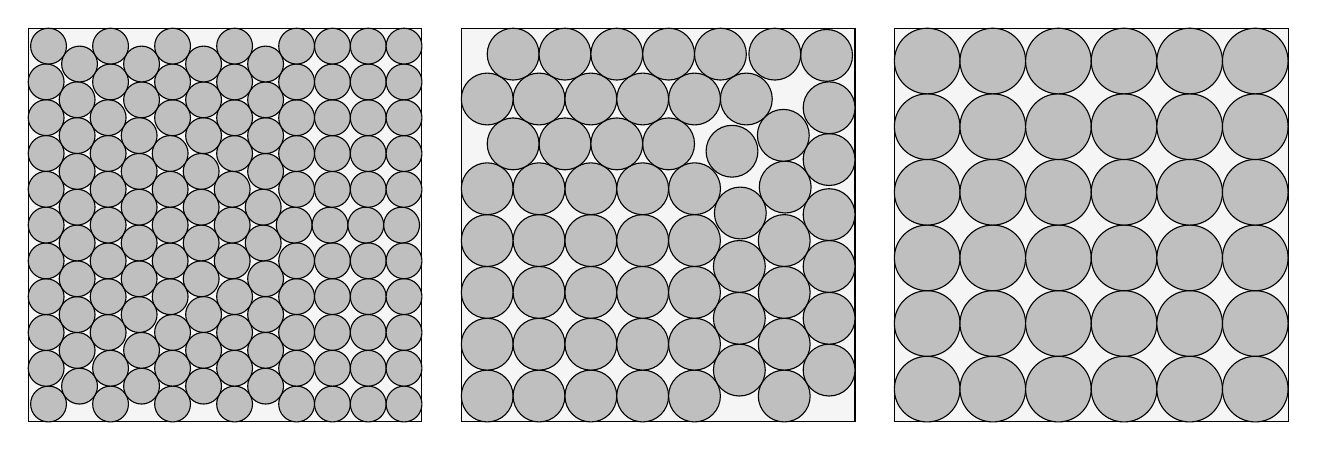
\begin{tikzpicture}[scale=5]
 	\begin{scope}[]
 	\fill[lightgray!15,draw=black] (0,0) rectangle (1,1);
 	\fill[lightgray,draw=black] (0.051591,0.0454733)circle(0.0454732);
 	\fill[lightgray,draw=black] (0.209115,0.0454733)circle(0.0454732);
 	\fill[lightgray,draw=black] (0.366639,0.0454733)circle(0.0454732);
 	\fill[lightgray,draw=black] (0.524163,0.0454733)circle(0.0454732);
 	\fill[lightgray,draw=black] (0.681687,0.0454733)circle(0.0454732);
 	\fill[lightgray,draw=black] (0.772634,0.0454733)circle(0.0454732);
 	\fill[lightgray,draw=black] (0.86358,0.0454733)circle(0.0454732);
 	\fill[lightgray,draw=black] (0.954527,0.0454733)circle(0.0454732);
 	\fill[lightgray,draw=black] (0.130353,0.0909465)circle(0.0454732);
 	\fill[lightgray,draw=black] (0.287877,0.0909465)circle(0.0454732);
 	\fill[lightgray,draw=black] (0.445401,0.0909465)circle(0.0454732);
 	\fill[lightgray,draw=black] (0.602925,0.0909465)circle(0.0454732);
 	\fill[lightgray,draw=black] (0.0454733,0.136214)circle(0.0454732);
 	\fill[lightgray,draw=black] (0.209115,0.13642)circle(0.0454732);
 	\fill[lightgray,draw=black] (0.366639,0.13642)circle(0.0454732);
 	\fill[lightgray,draw=black] (0.524163,0.13642)circle(0.0454732);
 	\fill[lightgray,draw=black] (0.681687,0.13642)circle(0.0454732);
 	\fill[lightgray,draw=black] (0.772634,0.13642)circle(0.0454732);
 	\fill[lightgray,draw=black] (0.86358,0.13642)circle(0.0454732);
 	\fill[lightgray,draw=black] (0.954527,0.13642)circle(0.0454732);
 	\fill[lightgray,draw=black] (0.124235,0.181687)circle(0.0454732);
 	\fill[lightgray,draw=black] (0.287877,0.181893)circle(0.0454732);
 	\fill[lightgray,draw=black] (0.445401,0.181893)circle(0.0454732);
 	\fill[lightgray,draw=black] (0.602925,0.181893)circle(0.0454732);
 	\fill[lightgray,draw=black] (0.0454733,0.22716)circle(0.0454732);
 	\fill[lightgray,draw=black] (0.202997,0.22716)circle(0.0454732);
 	\fill[lightgray,draw=black] (0.366639,0.227366)circle(0.0454732);
 	\fill[lightgray,draw=black] (0.524163,0.227366)circle(0.0454732);
 	\fill[lightgray,draw=black] (0.681687,0.227366)circle(0.0454732);
 	\fill[lightgray,draw=black] (0.772634,0.227366)circle(0.0454732);
 	\fill[lightgray,draw=black] (0.86358,0.227366)circle(0.0454732);
 	\fill[lightgray,draw=black] (0.954527,0.227366)circle(0.0454732);
 	\fill[lightgray,draw=black] (0.124235,0.272634)circle(0.0454732);
 	\fill[lightgray,draw=black] (0.281759,0.272634)circle(0.0454732);
 	\fill[lightgray,draw=black] (0.445401,0.27284)circle(0.0454732);
 	\fill[lightgray,draw=black] (0.602925,0.27284)circle(0.0454732);
 	\fill[lightgray,draw=black] (0.0454733,0.318107)circle(0.0454732);
 	\fill[lightgray,draw=black] (0.202997,0.318107)circle(0.0454732);
 	\fill[lightgray,draw=black] (0.360521,0.318107)circle(0.0454732);
 	\fill[lightgray,draw=black] (0.524163,0.318313)circle(0.0454732);
 	\fill[lightgray,draw=black] (0.681687,0.318313)circle(0.0454732);
 	\fill[lightgray,draw=black] (0.772634,0.318313)circle(0.0454732);
 	\fill[lightgray,draw=black] (0.86358,0.318313)circle(0.0454732);
 	\fill[lightgray,draw=black] (0.954527,0.318313)circle(0.0454732);
 	\fill[lightgray,draw=black] (0.124235,0.36358)circle(0.0454732);
 	\fill[lightgray,draw=black] (0.281759,0.36358)circle(0.0454732);
 	\fill[lightgray,draw=black] (0.439283,0.36358)circle(0.0454732);
 	\fill[lightgray,draw=black] (0.602925,0.363786)circle(0.0454732);
 	\fill[lightgray,draw=black] (0.0454733,0.409053)circle(0.0454732);
 	\fill[lightgray,draw=black] (0.202997,0.409053)circle(0.0454732);
 	\fill[lightgray,draw=black] (0.360521,0.409053)circle(0.0454732);
 	\fill[lightgray,draw=black] (0.518045,0.409053)circle(0.0454732);
 	\fill[lightgray,draw=black] (0.681687,0.409259)circle(0.0454732);
 	\fill[lightgray,draw=black] (0.772634,0.409259)circle(0.0454732);
 	\fill[lightgray,draw=black] (0.86358,0.409259)circle(0.0454732);
 	\fill[lightgray,draw=black] (0.954527,0.409259)circle(0.0454732);
 	\fill[lightgray,draw=black] (0.124235,0.454527)circle(0.0454732);
 	\fill[lightgray,draw=black] (0.281759,0.454527)circle(0.0454732);
 	\fill[lightgray,draw=black] (0.439283,0.454527)circle(0.0454732);
 	\fill[lightgray,draw=black] (0.596807,0.454527)circle(0.0454732);
 	\fill[lightgray,draw=black] (0.0454733,0.5)circle(0.0454732);
 	\fill[lightgray,draw=black] (0.202997,0.5)circle(0.0454732);
 	\fill[lightgray,draw=black] (0.360521,0.5)circle(0.0454732);
 	\fill[lightgray,draw=black] (0.518045,0.5)circle(0.0454732);
 	\fill[lightgray,draw=black] (0.675569,0.5)circle(0.0454732);
 	\fill[lightgray,draw=black] (0.766516,0.5)circle(0.0454732);
 	\fill[lightgray,draw=black] (0.857462,0.5)circle(0.0454732);
 	\fill[lightgray,draw=black] (0.948409,0.5)circle(0.0454732);
 	\fill[lightgray,draw=black] (0.124235,0.545473)circle(0.0454732);
 	\fill[lightgray,draw=black] (0.281759,0.545473)circle(0.0454732);
 	\fill[lightgray,draw=black] (0.439283,0.545473)circle(0.0454732);
 	\fill[lightgray,draw=black] (0.596807,0.545473)circle(0.0454732);
 	\fill[lightgray,draw=black] (0.681687,0.590741)circle(0.0454732);
 	\fill[lightgray,draw=black] (0.772634,0.590741)circle(0.0454732);
 	\fill[lightgray,draw=black] (0.86358,0.590741)circle(0.0454732);
 	\fill[lightgray,draw=black] (0.954527,0.590741)circle(0.0454732);
 	\fill[lightgray,draw=black] (0.0454733,0.590947)circle(0.0454732);
 	\fill[lightgray,draw=black] (0.202997,0.590947)circle(0.0454732);
 	\fill[lightgray,draw=black] (0.360521,0.590947)circle(0.0454732);
 	\fill[lightgray,draw=black] (0.518045,0.590947)circle(0.0454732);
 	\fill[lightgray,draw=black] (0.602925,0.636214)circle(0.0454732);
 	\fill[lightgray,draw=black] (0.124235,0.63642)circle(0.0454732);
 	\fill[lightgray,draw=black] (0.281759,0.63642)circle(0.0454732);
 	\fill[lightgray,draw=black] (0.439283,0.63642)circle(0.0454732);
 	\fill[lightgray,draw=black] (0.524163,0.681687)circle(0.0454732);
 	\fill[lightgray,draw=black] (0.681687,0.681687)circle(0.0454732);
 	\fill[lightgray,draw=black] (0.772634,0.681687)circle(0.0454732);
 	\fill[lightgray,draw=black] (0.86358,0.681687)circle(0.0454732);
 	\fill[lightgray,draw=black] (0.954527,0.681687)circle(0.0454732);
 	\fill[lightgray,draw=black] (0.0454733,0.681893)circle(0.0454732);
 	\fill[lightgray,draw=black] (0.202997,0.681893)circle(0.0454732);
 	\fill[lightgray,draw=black] (0.360521,0.681893)circle(0.0454732);
 	\fill[lightgray,draw=black] (0.445401,0.72716)circle(0.0454732);
 	\fill[lightgray,draw=black] (0.602925,0.72716)circle(0.0454732);
 	\fill[lightgray,draw=black] (0.124235,0.727366)circle(0.0454732);
 	\fill[lightgray,draw=black] (0.281759,0.727366)circle(0.0454732);
 	\fill[lightgray,draw=black] (0.366639,0.772634)circle(0.0454732);
 	\fill[lightgray,draw=black] (0.524163,0.772634)circle(0.0454732);
 	\fill[lightgray,draw=black] (0.681687,0.772634)circle(0.0454732);
 	\fill[lightgray,draw=black] (0.772634,0.772634)circle(0.0454732);
 	\fill[lightgray,draw=black] (0.86358,0.772634)circle(0.0454732);
 	\fill[lightgray,draw=black] (0.954527,0.772634)circle(0.0454732);
 	\fill[lightgray,draw=black] (0.0454733,0.77284)circle(0.0454732);
 	\fill[lightgray,draw=black] (0.202997,0.77284)circle(0.0454732);
 	\fill[lightgray,draw=black] (0.287877,0.818107)circle(0.0454732);
 	\fill[lightgray,draw=black] (0.445401,0.818107)circle(0.0454732);
 	\fill[lightgray,draw=black] (0.602925,0.818107)circle(0.0454732);
 	\fill[lightgray,draw=black] (0.124235,0.818313)circle(0.0454732);
 	\fill[lightgray,draw=black] (0.209115,0.86358)circle(0.0454732);
 	\fill[lightgray,draw=black] (0.366639,0.86358)circle(0.0454732);
 	\fill[lightgray,draw=black] (0.524163,0.86358)circle(0.0454732);
 	\fill[lightgray,draw=black] (0.681687,0.86358)circle(0.0454732);
 	\fill[lightgray,draw=black] (0.772634,0.86358)circle(0.0454732);
 	\fill[lightgray,draw=black] (0.86358,0.86358)circle(0.0454732);
 	\fill[lightgray,draw=black] (0.954527,0.86358)circle(0.0454732);
 	\fill[lightgray,draw=black] (0.0454733,0.863786)circle(0.0454732);
 	\fill[lightgray,draw=black] (0.130353,0.909053)circle(0.0454732);
 	\fill[lightgray,draw=black] (0.287877,0.909053)circle(0.0454732);
 	\fill[lightgray,draw=black] (0.445401,0.909053)circle(0.0454732);
 	\fill[lightgray,draw=black] (0.602925,0.909053)circle(0.0454732);
 	\fill[lightgray,draw=black] (0.051591,0.954527)circle(0.0454732);
 	\fill[lightgray,draw=black] (0.209115,0.954527)circle(0.0454732);
 	\fill[lightgray,draw=black] (0.366639,0.954527)circle(0.0454732);
 	\fill[lightgray,draw=black] (0.524163,0.954527)circle(0.0454732);
 	\fill[lightgray,draw=black] (0.681687,0.954527)circle(0.0454732);
 	\fill[lightgray,draw=black] (0.772634,0.954527)circle(0.0454732);
 	\fill[lightgray,draw=black] (0.86358,0.954527)circle(0.0454732);
 	\fill[lightgray,draw=black] (0.954527,0.954527)circle(0.0454732);
 	\end{scope}[]
 	\begin{scope}[shift={(1.1,0)}]
 	\fill[lightgray!15,draw=black] (0,0) rectangle (1,1);
 	\fill[lightgray,draw=black] (0.0658075,0.0658075)circle(0.0658074);
 	\fill[lightgray,draw=black] (0.197422,0.0658075)circle(0.0658074);
 	\fill[lightgray,draw=black] (0.329037,0.0658075)circle(0.0658074);
 	\fill[lightgray,draw=black] (0.460652,0.0658075)circle(0.0658074);
 	\fill[lightgray,draw=black] (0.592267,0.0658075)circle(0.0658074);
 	\fill[lightgray,draw=black] (0.820231,0.0658075)circle(0.0658074);
 	\fill[lightgray,draw=black] (0.706249,0.131615)circle(0.0658074);
 	\fill[lightgray,draw=black] (0.934193,0.131651)circle(0.0658074);
 	\fill[lightgray,draw=black] (0.0658075,0.197422)circle(0.0658074);
 	\fill[lightgray,draw=black] (0.197422,0.197422)circle(0.0658074);
 	\fill[lightgray,draw=black] (0.329037,0.197422)circle(0.0658074);
 	\fill[lightgray,draw=black] (0.460652,0.197422)circle(0.0658074);
 	\fill[lightgray,draw=black] (0.592267,0.197422)circle(0.0658074);
 	\fill[lightgray,draw=black] (0.820211,0.197458)circle(0.0658074);
 	\fill[lightgray,draw=black] (0.706229,0.263266)circle(0.0658074);
 	\fill[lightgray,draw=black] (0.934193,0.263266)circle(0.0658074);
 	\fill[lightgray,draw=black] (0.0658075,0.329037)circle(0.0658074);
 	\fill[lightgray,draw=black] (0.197422,0.329037)circle(0.0658074);
 	\fill[lightgray,draw=black] (0.329037,0.329037)circle(0.0658074);
 	\fill[lightgray,draw=black] (0.460652,0.329037)circle(0.0658074);
 	\fill[lightgray,draw=black] (0.820211,0.329073)circle(0.0658074);
 	\fill[lightgray,draw=black] (0.592267,0.329109)circle(0.0658074);
 	\fill[lightgray,draw=black] (0.934193,0.394881)circle(0.0658074);
 	\fill[lightgray,draw=black] (0.706249,0.394917)circle(0.0658074);
 	\fill[lightgray,draw=black] (0.0658075,0.460652)circle(0.0658074);
 	\fill[lightgray,draw=black] (0.197422,0.460652)circle(0.0658074);
 	\fill[lightgray,draw=black] (0.329037,0.460652)circle(0.0658074);
 	\fill[lightgray,draw=black] (0.460652,0.460652)circle(0.0658074);
 	\fill[lightgray,draw=black] (0.592267,0.460724)circle(0.0658074);
 	\fill[lightgray,draw=black] (0.820231,0.460724)circle(0.0658074);
 	\fill[lightgray,draw=black] (0.934193,0.526568)circle(0.0658074);
 	\fill[lightgray,draw=black] (0.708711,0.530623)circle(0.0658074);
 	\fill[lightgray,draw=black] (0.329109,0.592267)circle(0.0658074);
 	\fill[lightgray,draw=black] (0.460724,0.592267)circle(0.0658074);
 	\fill[lightgray,draw=black] (0.0658075,0.592267)circle(0.0658074);
 	\fill[lightgray,draw=black] (0.197422,0.592267)circle(0.0658074);
 	\fill[lightgray,draw=black] (0.592463,0.592339)circle(0.0658074);
 	\fill[lightgray,draw=black] (0.822673,0.596466)circle(0.0658074);
 	\fill[lightgray,draw=black] (0.934193,0.666365)circle(0.0658074);
 	\fill[lightgray,draw=black] (0.687571,0.687571)circle(0.0658074);
 	\fill[lightgray,draw=black] (0.263266,0.706229)circle(0.0658074);
 	\fill[lightgray,draw=black] (0.394917,0.706249)circle(0.0658074);
 	\fill[lightgray,draw=black] (0.526532,0.706249)circle(0.0658074);
 	\fill[lightgray,draw=black] (0.131615,0.706249)circle(0.0658074);
 	\fill[lightgray,draw=black] (0.817898,0.727995)circle(0.0658074);
 	\fill[lightgray,draw=black] (0.934192,0.79798)circle(0.0658074);
 	\fill[lightgray,draw=black] (0.197458,0.820211)circle(0.0658074);
 	\fill[lightgray,draw=black] (0.329073,0.820211)circle(0.0658074);
 	\fill[lightgray,draw=black] (0.592375,0.820211)circle(0.0658074);
 	\fill[lightgray,draw=black] (0.72399,0.820211)circle(0.0658074);
 	\fill[lightgray,draw=black] (0.460724,0.820231)circle(0.0658074);
 	\fill[lightgray,draw=black] (0.0658075,0.820231)circle(0.0658074);
 	\fill[lightgray,draw=black] (0.927873,0.930974)circle(0.0658074);
 	\fill[lightgray,draw=black] (0.796298,0.934192)circle(0.0658074);
 	\fill[lightgray,draw=black] (0.131651,0.934193)circle(0.0658074);
 	\fill[lightgray,draw=black] (0.263266,0.934193)circle(0.0658074);
 	\fill[lightgray,draw=black] (0.394881,0.934193)circle(0.0658074);
 	\fill[lightgray,draw=black] (0.526568,0.934193)circle(0.0658074);
 	\fill[lightgray,draw=black] (0.658183,0.934193)circle(0.0658074);
 	\end{scope}[]
 	\begin{scope}[shift={(2.2,0)}]
 	\fill[lightgray!15,draw=black] (0,0) rectangle (1,1);
 	\fill[lightgray,draw=black] (0.0833333,0.0833333)circle(0.0833333333);
 	\fill[lightgray,draw=black] (0.25,0.0833333)circle(0.0833333333);
 	\fill[lightgray,draw=black] (0.416667,0.0833333)circle(0.0833333333);
 	\fill[lightgray,draw=black] (0.583333,0.0833333)circle(0.0833333333);
 	\fill[lightgray,draw=black] (0.75,0.0833333)circle(0.0833333333);
 	\fill[lightgray,draw=black] (0.916667,0.0833333)circle(0.0833333333);
 	\fill[lightgray,draw=black] (0.0833333,0.25)circle(0.0833333333);
 	\fill[lightgray,draw=black] (0.25,0.25)circle(0.0833333333);
 	\fill[lightgray,draw=black] (0.416667,0.25)circle(0.0833333333);
 	\fill[lightgray,draw=black] (0.583333,0.25)circle(0.0833333333);
 	\fill[lightgray,draw=black] (0.75,0.25)circle(0.0833333333);
 	\fill[lightgray,draw=black] (0.916667,0.25)circle(0.0833333333);
 	\fill[lightgray,draw=black] (0.0833333,0.416667)circle(0.0833333333);
 	\fill[lightgray,draw=black] (0.25,0.416667)circle(0.0833333333);
 	\fill[lightgray,draw=black] (0.416667,0.416667)circle(0.0833333333);
 	\fill[lightgray,draw=black] (0.583333,0.416667)circle(0.0833333333);
 	\fill[lightgray,draw=black] (0.75,0.416667)circle(0.0833333333);
 	\fill[lightgray,draw=black] (0.916667,0.416667)circle(0.0833333333);
 	\fill[lightgray,draw=black] (0.0833333,0.583333)circle(0.0833333333);
 	\fill[lightgray,draw=black] (0.25,0.583333)circle(0.0833333333);
 	\fill[lightgray,draw=black] (0.416667,0.583333)circle(0.0833333333);
 	\fill[lightgray,draw=black] (0.583333,0.583333)circle(0.0833333333);
 	\fill[lightgray,draw=black] (0.75,0.583333)circle(0.0833333333);
 	\fill[lightgray,draw=black] (0.916667,0.583333)circle(0.0833333333);
 	\fill[lightgray,draw=black] (0.0833333,0.75)circle(0.0833333333);
 	\fill[lightgray,draw=black] (0.25,0.75)circle(0.0833333333);
 	\fill[lightgray,draw=black] (0.416667,0.75)circle(0.0833333333);
 	\fill[lightgray,draw=black] (0.583333,0.75)circle(0.0833333333);
 	\fill[lightgray,draw=black] (0.75,0.75)circle(0.0833333333);
 	\fill[lightgray,draw=black] (0.916667,0.75)circle(0.0833333333);
 	\fill[lightgray,draw=black] (0.0833333,0.916667)circle(0.0833333333);
 	\fill[lightgray,draw=black] (0.25,0.916667)circle(0.0833333333);
 	\fill[lightgray,draw=black] (0.416667,0.916667)circle(0.0833333333);
 	\fill[lightgray,draw=black] (0.583333,0.916667)circle(0.0833333333);
 	\fill[lightgray,draw=black] (0.75,0.916667)circle(0.0833333333);
 	\fill[lightgray,draw=black] (0.916667,0.916667)circle(0.0833333333);
 	
 	\end{scope}[]
 	\end{tikzpicture}
 	\caption{Most efficient distributions for circle packing for $d=0.1$, $d=0.15$,$d=0.2$.}
 	\label{fig:packing} 
 \end{figure}


With the exception of the latter, these values are yet to be proven to be optimal. However, the optimal values are not expected to be very different, as the remaining area is very limited. The


%----------------------------------------------------------------------------------------
%	THESIS CONTENT - APPENDICES
%----------------------------------------------------------------------------------------

%\addtocontents{toc}{\vspace{2em}} % Add a gap in the Contents, for aesthetics

%\appendix % Cue to tell LaTeX that the following 'chapters' are Appendices

% Include the appendices of the thesis as separate files from the Appendices folder
% Uncomment the lines as you write the Appendices

%% Appendix A

\chapter{Appendix Title Here} % Main appendix title

\label{AppendixA} % For referencing this appendix elsewhere, use \ref{AppendixA}

\lhead{Appendix A. \emph{Appendix Title Here}} % This is for the header on each page - perhaps a shortened title

Write your Appendix content here.
%\input{Appendices/AppendixB}
%\input{Appendices/AppendixC}

\addtocontents{toc}{\vspace{2em}} % Add a gap in the Contents, for aesthetics

\backmatter

%----------------------------------------------------------------------------------------
%	BIBLIOGRAPHY
%----------------------------------------------------------------------------------------

\label{References}

\renewcommand\bibname{References}

\lhead{\emph{References}} % Change the page header to say "Bibliography"

\bibliographystyle{abbrvnat} % Use the "unsrtnat" BibTeX style for formatting the Bibliography

\bibliography{Bibliography} % The references (bibliography) information are stored in the file named "Bibliography.bib"

\end{document}  